\documentclass[11pt]{article}

% this is the template for an issue of the Data Engineering Bulletin

% all packages used by any paper must be listed here

%\usepackage{hyperref}
\usepackage{authblk}
\setlength{\affilsep}{0em}
\usepackage{inputenc}
\usepackage{debulletin}
\usepackage{times}
\usepackage{graphicx}
\usepackage{array}
\usepackage{wrapfig}
\usepackage[table]{xcolor}
\usepackage{tcolorbox}
\usepackage{amssymb}
%\usepackage[labelfont=bf,labelsep=space,list=true]{subcaption}
\usepackage{url}
\usepackage{mathtools, bm}
\usepackage{float}
\usepackage{multirow}
\usepackage{multicol}
\usepackage{algorithm}
\usepackage{subfig}
\usepackage{algpseudocode}
\setlength{\intextsep}{10pt plus 2pt minus 2pt}
\hyphenation{finally}

\begin{document}


% please enter real date, vol no, issue no
\bulletindate{Mar 2020}
\bulletinvolume{43}
\bulletinnumber{1}
\bulletinyear{2020}

% these are files that I have- but your part of the issue can be done without
% them
\IEEElogo{cs.pdf}
\insidefrontcover{incvA19.pdf}
%\insidebackcover[ICDE Conference]{./calls/icde-new-a.ps}

\begin{bulletin}

% the above samples assume the issue is generated from a directory structure of the following sort
% major directory name is month and year of issue
% there are sub-directorys for
% letters: directory name is "letters"
% technical articles: a directory per paper, named for an "author"
% news articles: directory name is "news"
% calls: directory name is "calls

%
%  Editor letters section.  Use the lettersection environment.
%  Each letter is contained in a letter environment, where the two required
%  options to \begin{letter} are the author and the address of the author.
%

\begin{lettersection}

% there will be other letters- and a blank page will appear in your document
% but the special issue part will be fine

\begin{letter}{Letter from the Editor-in-Chief}
{Haixun Wang}{WeWork Corporation}
\documentclass[11pt]{article} 

\usepackage{deauthor,times,graphicx}
%\usepackage{url}
\usepackage{hyperref}

\begin{document}


\section*{Thank You, David!}

I know I represent the readers, the associate editors, and also the
broad database community when I say we are extremely grateful to David
Lomet for his distinguished and dedicated service as the
Editor-in-Chief of the Data Engineering Bulletin for the last 26
years.

Since its launch in 1977, the Bulletin has produced a total of 154
issues. Reading through the topics of the past issues that spanned
more than four decades makes me feel nothing short of amazing. They
show not just how far the database research has come, but to a certain
extent, how much the entire field of computer science and the IT
industry have evolved. While important topics never fail to arise in
the Bulletin in a timely fashion, it is also interesting to observe in
the 154 issues many recurring topics, including query optimization,
spatial and temporal data management, data integration, etc. It proves
that the database research has a solid foundation that supports many
new applications, and at the same time, it demonstrates that the
database research is constantly reinventing itself to meet the
challenges of the time. What the Bulletin has faithfully documented
over the last 42 years is nothing else but this amazing effort.

Among the 154 issues since the launch of the Bulletin, David had been
the Editor-in-Chief for 103 of them. This itself is a phenomenal
record worth an extra-special celebration. But more importantly, David
shaped the discussions and the topics in the long history of the
Bulletin.  I had the honor to work with David in 2016 and 2017 when I
served as the associate editor for two Bulletin issues. What was most
appealing to me was the opportunity of working with the top experts on
a topic that I am passionate about. The Bulletin is truly unique in
this aspect.

I understand the responsibility and the expectation of the
Editor-in-Chief, especially after David set such a great example in
the last 26 years. I thank David and the associate editors for their
trust, and I look forward to working with authors, readers, and the
database community on the future issues of the Data Engineering
Bulletin.

%\begin{flushright}
%Haixun Wang\\
%WeWork
%\end{flushright}
\end{document}


\end{letter}
%
\newpage
%
%% your introductory letter goes here
%
\begin{letter}{Letter from the Special Issue Editor}
{Philippe Bonnet}{IT University of Copenhagen}
\documentclass[11pt]{article} 

\usepackage{deauthor,times,graphicx}
%\usepackage{url}

\begin{document}

Scientific computing used to be based on numerical simulations run on mid-range warehouse scale computers.
This is no longer the case, due to the combination of strong application pull and technology push.
 
In order to get realistic models of a phenomenon in natural or engineered systems, scientists 
must analyze unprecedented volumes of data generated by new generations of instruments and experiments.
In addition, they must run simulations at higher spatial resolutions, for longer simulation times and with 
higher dimension models, possibly combining multiple physical models of a phenomenon, or study multiple 
simultaneous phenomena. These new computational challenges stemming from scientific applicatins
 have triggered a convergence of traditional
numerical simulation with machine learning and high-performance data analytics. Put differently,
data science and eScience are merging. 

The technology push is due to the planned transition to Exascale systems.
Strictly defined, Exascale computers are capable of $10^{18}$ floating points operations per second (flops).
More interestingly, they are three orders of magnitude faster than the High-Performance Computers deployed
a decade ago. 
The first Exascale systems are expected in the coming year. In the US, three systems are
being deployed: Aurora at Argonne National Lab, 
Frontier at Oak Ridge National Lab and El Capitan at Lawrence Livermore Lab. In China 
three existing pre-exascale systems are being extended: Sunway at the National Research Center of Parallel 
Computer Engineering and Technology (NRCPC in Wuxi, Jiangsu), Sugon (installed at the Shanghai Supercomputer
Center)  and Tianhe at the National Center 
of Defense Technology (NUDT in Changsha, Hunan).
In Japan, Riken and Fujitsu have designed the Fugaku Exascale computer, which has been announced for 2021, 2022. It
will be hosted at the RIKEN Center for Computational Science in Kobe.
In Europe, three pre-exascale computers are under construction: Mare Nostrum 5 at the Barcelona Supercomputing Center,
Leonardo at Bologna's CINECA and LUMI at the CSC Data Center in Kaajani, Finland.

In 2008, Kogge et al. surveyed the technology challenges in achieving Exascale systems.
The main roadblock they identified was {\em transporting data from one site to another: on the same chip, 
between closely coupled chips in a common package, or between different racks on opposite sides of a large
machine room.} Put differently, minimizing data movement is the key challenge on Exascale systems.
This is a challenge in terms of architecture, but it is also a challenge for data management.

In this issue, leading researchers from the HPC and database communities present their work on data management 
at Exascale. The papers will give readers an insight in the nature of the application pull and technology push
sketched above. They contain the lessons learnt at the forefront of scientific data management. They are very
interesting points of departure for future work.

Mario Lassnig from CERN and his co-authors review their experience with the Rucio system, developed at CERN,
to handle data in the ATLAS experiment. They detail the challenges they faced and how Rucio addresses
them. They report on recent efforts to adapt Rucio in the context of other large-scale scientific projects.

Jerome Soumagne from HDF Group and his co-authors tackle the issue of performance and resilience for data services at Exascale.
They propose Remote Procedure Call as a building block for such data services. The paper describes the design
of Mercury, a new form of Remote Procedure Call adapted to large data transfers on low-latency network fabrics. 

Jeremy Logan from Oak Ridge National Lab and his co-authors focus on ADIOS, the Adaptable I/O System, that
provides a publish/subscribe abstraction for high-performance data services. The paper describe its design and
its use in the context of near Exascale use cases. Based on lessons learnt and examples from a range of different
projects, the authors discuss challenges and opportunities for future work on data management at Exascale.

Noel Moreno Lemus from LNCC (National Lab for Scientific Computing in Rio de Janeiro, Brazeil) and his co-authors tackle the issue of large-scale spatio-temporal simulations. More specifically,
they focus on answering uncertainty quantification queries over such simulation results. This is a great
example of the convergence of numerical simulation and query processing.

Finally, Alberto Lerner from the eXascale Infolab at U.Fribourg and his co-authors present their
vision for in-network computing and near-storage processing. These techniques are crucial for bringing
computation closer to data and thus tackle the issue of data movement. Their vision is based on a thorough analysis
of the current generation of platforms and of the computation tasks that could be brought closer to data at rest
or in movement.

These papers addresses several aspects of the state of the art in data management at Exascale and
they outline a range of challenges. There
are many opportunities for the database community to engage with the high-performance computing community
to tackle these challenges. As Jim Gray once wrote: {\em The next decade will be exciting}! 

Working on this issue has been a privilege. I would like to thank the authors, and specially the five contact
authors for their diligence and express my admiration for the quality of their work. I would also like to thank
Haixun Wang for his kind and efficient management and Pinar Tözün for her feedback. Finally, 
I would like to thank David Lomet for the opportunity
to act as editor of this special issue.

\end{document}


\end{letter}

\end{lettersection}

% put the name of your special issue below

\begin{opinionsection}
\begin{opinion}{Entities with Quantities}
{Gerhard Weikum}{Max Planck Institute for Informatics}
\documentclass[11pt]{article}
\usepackage{deauthor,times,graphicx,url} 


%% \newlength{\bibitemsep}\setlength{\bibitemsep}{.2\baselineskip plus .05\baselineskip minus .05\baselineskip}
%% \newlength{\bibparskip}\setlength{\bibparskip}{0pt}
%% \let\oldthebibliography\thebibliography
%% \renewcommand\thebibliography[1]{%
%%   \oldthebibliography{#1}%
%%   \setlength{\parskip}{\bibitemsep}%
%%   \setlength{\itemsep}{\bibparskip}%
%% }
%% \setlength{\bibitemsep}{.1\baselineskip plus .05\baselineskip minus .05\baselineskip}



\newcommand{\squishlist}{
 \begin{list}{$\bullet$}
  { \setlength{\itemsep}{0pt}
     \setlength{\parsep}{1pt}
     \setlength{\topsep}{1pt}
     \setlength{\partopsep}{0pt}
     \setlength{\leftmargin}{1.5em}
     \setlength{\labelwidth}{1em}
     \setlength{\labelsep}{0.5em} } }
 \newcommand{\squishend}{\end{list}}


\begin{document}
\title{Entities with Quantities} %5-8 pages
\author{Gerhard Weikum\\Max Planck Institute for Informatics\\Saarland Informatics Campus E1.4, Saarbr\"ucken, Germany\\weikum@mpi-inf.mpg.de}

%\maketitle


%\section*{The Web as a Database !?}
\subsection*{The Web as a Database }

Unstructured content, like text in web pages, and semistructured content, like HTML tables in web pages, has much weaker search functionality compared to structured databases. For example, joins between text documents via co-occurring entity mentions or attribute values are infeasible, unless major efforts are taken to create mark-up for a structured view. As for web tables, filters on entity mentions allow users to look up data, but results are noisy and 
error-prone because of ad-hoc choices for names of entities and value encodings, with huge heterogeneity across tables and often even within a table. 

In the last few years, large knowledge graphs (KG), 
machine learning (ML) techniques and advances in entity linking algorithms \cite{Mudgal:SIGMOD2018,Shen:TKDE2015}
have enabled search engines to overcome these issues, to a large degree \cite{Noy:CACM2019}.
By detecting entity mentions in web content and normalizing them onto KG entries, it has become possible to answer entity-centric queries about people, places and products almost as precisely and concisely as  a database query.
%As illustration of these impressive advances,
The following examples work with all major search engines and return
crisp entity-level answers:

%\vspace*{0.05cm}
\begin{center}
{\small
\begin{tabular}{|l|l|}\hline
Query & Results(s) \\ \hline
Height of the Eiffel Tower & 324 meters\\
highest building in Paris & Eiffel Tower\\
CEO of Amazon & Jeff Bezos\\
Bezos worth & 108.9 Billion USD\\
CEOs of IT companies &  Jeff Bezos, Sundar Pichai, Ginny Rometti, Zhang Yong, \dots\\ \hline
\end{tabular}
}
\end{center}

Search engines leverage look-ups in back-end knowledge graphs,
and run entity detection on both user inputs and page contents
to provide these answers.
It seems that entity-centric search on the web has become as easy and 
as effective as querying a structured and curated database!

The same methodologies, particularly, entity linking,
are also key to joining data for the same entity
across web tables and
within heterogeneous data lakes \cite{Lehmberg:PVLDB2017,Zhu:SIGMOD2019}.
%%%cite Halevy here as well ???


\subsection*{Quantity Queries}

On the disillusioning side, there is an interesting and challenging type of queries
that is underexplored and hardly supported:
searching with {\em quantities}: quantitative measures of entities
that capture financial, physical, technological or environmental properties.
Examples are: 
%\squishlist
a celebrity's personal wealth,
a company's quarterly revenue, 
 a car's energy consumption,
 a material's thermal conductivity, or
 the usual and maximal dosage of a medical drug.
%\squishend
%\noindent 
Quantities can be represented as
$\langle measure, value, unit \rangle$ triples,
such as $\langle height, 8848, meter \rangle$.
The units can be simple, such as meters, light-years, US dollars, Euros etc.,
with well-defined conversion rules between different units for the
same measure. But they can also be quite sophisticated such as
{\em kWh/100km} for a car's energy consumption or 
{\em W/(mK)}
for the thermal conductivity of materials,
with more complex conversion rules, e.g., between
kWh/100km and MPG (miles per gallon) for electric, hybrid and fuel-based cars.
Conversions often require context information, such as
date for currency conversions, or location for car properties
(incl. carbon footprint).
The International System of Units (SI) is a rich reference for
measures and conversions 
%({\small\tt en.wikipedia.org/wiki/International\_System\_of\_Units}).
({\small\url{https://en.wikipedia.org/wiki/International_System_of_Units}}).

Search engines perform well on looking up quantities for given entities, such as
retrieving the height of the Eiffel Tower. In this regard, quantity properties
are not different from other properties such as city or architect.
The pain point, however, is {\em finding} all entities (of a certain type) that
satisfy a {\em search condition for a quantity of interest},
for example, buildings taller than 500m or runners completing a marathon under 2:10h. 
With few exceptions where explicit lists are available, search engines
fall back to returning page links only.
%and leave further reading of these pages
%to the user. 
The following examples illustrate this disappointing behavior.


%\vspace*{0.05cm}
\begin{center}
{\small
\begin{tabular}{|p{5cm}|p{10cm}|}\hline
Query & Results(s) \\ \hline\hline
people worth 50 Billion USD & link to ``List of Americans by net worth - Wikipedia'' \\ \hline
\dots more than 50 Billion USD & links to pages such as
``Meet the world's 50 richest billionaires in 2019''\\ \hline
\dots between 10 and 50 Billion Euros & links to pages such as
``Inequality and Wealth Distribution in Germany'' \\ \hline
\end{tabular}
}
\end{center}

Search engines do not understand numbers and units (with a few exceptions
regarding dates and money, sometimes). For example, ``15 kW'' and
``15.000 W'' are two different strings.
Units like ``l/100km'', 
``MPG'', ``MPGe'' and ``kWh/100km'' are also just strings, and the systems are
%agnostic of the option for unit conversion.
ignorant about unit conversions.

These queries would be trivial to handle if all data resided
in a single database with well-designed schema,
standardized value encodings, and high-quality curation.
However, these databases do rarely exist, or are outdated or incomplete.
One would hope that this is where encyclopedic knowledge graphs
kick in, such as DBpedia, Wikidata or Yago.
However, quantitative properties are very sparse in these KGs,
and often represented just as strings, e.g., ``250 mi $\pm$ 10''
for the range of a car model.
Only Wikidata contains triples for the range of cars, but only for
4 models (as of Dec. 2019). 
As for other measures, like engine power, energy efficiency, carbon footprint etc.,
none of these KGs has any data.
% on such properties.
Only the Web as a whole contains the wealth of information that
is needed to compute accurate and complete answers to
many kinds of quantity queries.





%%%%%%%%%%%%%%%%%%%%%%%%%%%%%%%%%%%

\subsection*{Initial Proof of Concept}

Supporting quantity queries is easy over a 
single well-curated database. It is challenging over
web page contents, 
%and equally difficult over 
web table 
collections or data lakes.
%database federations.
%It is a daunting challenge when considering large data lakes,
%as they 
In the latter cases, we need to overcome the
obstacles of
highly heterogeneous schemas,
diverse and noisy value encodings, and widely varying degrees of
coverage \cite{Miller:DEbull2018}.
%\cite{Nargesian:PVLDB2018}.
%%%check if this is the best reference here
%(e.g., Open Data \cite{Nargesian:PVLDB2018}).

As an initial effort,
% in this research direction, 
we devised methods for
a limited class of quantity queries over text document collections such as
Wikipedia articles or news corpora. This work has led to an early
prototype system, called {\em Qsearch} \cite{Ho:ISWC2019,Ho:WSDM2020}.
The system consists of a {\em data preparation} stage with quantity extraction
and indexing, and a {\em query processing} stage with matching and ranking.
A Qsearch demonstrator is accessible at
{\small\url{https://qsearch.mpi-inf.mpg.de}}. 
Figure \ref{fig1-qsearch-screenshot} shows the top-ranked answers
for an example query about buildings higher than 1000 ft.

\begin{figure} [tb]
  \centering
   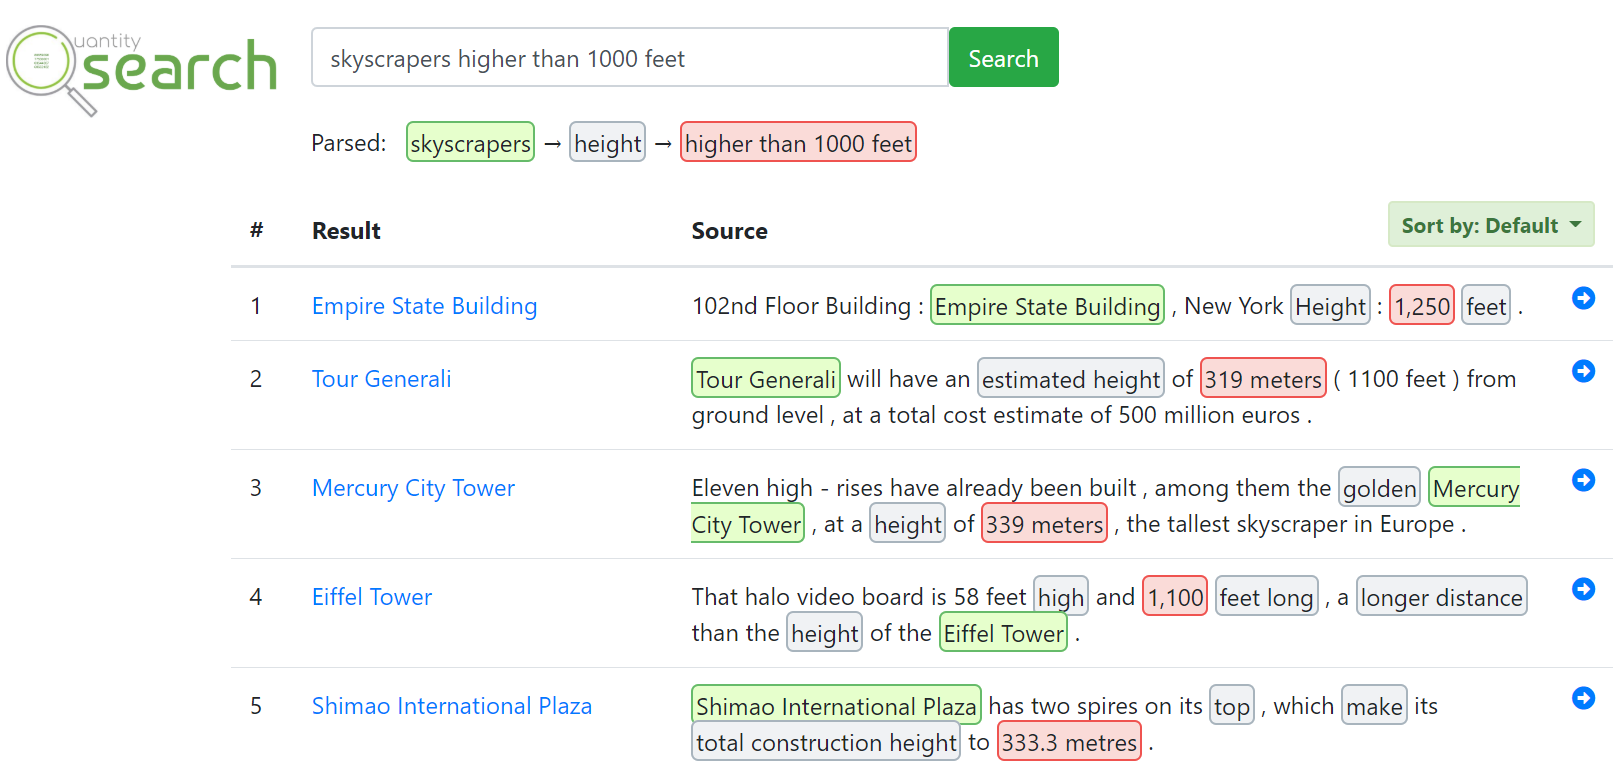
\includegraphics[width=0.8\textwidth]{letters/fig1-qsearch-screenshot.png}
\vspace*{-0.3cm} 
     \caption{Screenshot of Qsearch answers to query about buildings higher than 1000 ft}
      \label{fig1-qsearch-screenshot}
\end{figure}

\vspace{0.2cm}
\noindent{\bf Information Extraction:}
Qsearch 
%processes textual context one sentence at a time, using
uses
machine learning for sequence tagging. 
It trains an LSTM neural network with distant supervision,
and applies the learned model to tag each word in a sentence,
identifying three components:
i) an {\em entity} of interest, ii) a {\em quantity} that refers to this entity,
and iii) {\em context cues} that capture what exactly the quantity denotes.
For example, from the sentence
``The hybrid Prius is sold in Germany for less than 30 thousand, and
has a battery only range of 60 km.'',
Qsearch extracts two assertions:
first, related to price: i) Toyota Prius as key entity, 
ii) 30,000 Euros (upper bound) as quantity,
iii) ``sold in Germany'' as cue words,
and second, related to range: i) Toyota Prius as entity,
ii) 60 km as quantity, 
iii) ``battery only range'' as cue words.
%Entities are linked to a knowledge graph, this way canonicalizing their names,
%and quantities are normalized in a best-effort way, with units inferred when possible.
%All extracted assertions are indexed on all components.

\vspace{0.2cm}
\noindent{\bf Query Analysis:}
At query time, Qsearch analyzes telegraphic queries or full questions and 
decomposes them into three components:
{\em semantic target type} (e.g., buildings or hybrid cars etc.),
{\em quantity condition} of the form $\langle comparison, value, unit \rangle$
(with comparisons like $\le$, $\ge$, {between}, etc.),
{\em context cues} that candidate results should match (e.g., ``electric range in city traffic''
for a query about hybrid cars).

\vspace{0.2cm}
\noindent{\bf Matching and Ranking:}
Query processing aims to match all components of an assertion against the
components of the query: the entity must be of the right type,
the quantity condition must be satisfied, and the context cues must match
as well as possible (leveraging word embeddings, e.g., to capture the
relatedness of ``battery only'' and ``electric range'').
As the latter comes with uncertainty, Qsearch employs 
language-model-style ranking to compute the best answers.


%%%%%%%%%%%%%%%%%%%%%%%%%%%%%%%%


\subsection*{Challenges and Opportunities}

\noindent{\bf Quantity Filters:}
%
%extraction from text
Even basic filters over quantities still pose enormous challenges.
The extraction from text often faces complicated and misleading inputs, 
such as ``The battery of the hybrid Toyoto Prius lasts well over 100,000 miles''
as a spurious candidate for the electric range of this car.
For more sophisticated measures such as the CO2 footprint of cars, 
it is crucial to consider elaborate context like the source of energy for
electric cars, the driving situations (city vs. highway, summer vs. winter),
and more. This will rarely be fully captured in a single sentence;
so we need information extraction that combines and reconciles cues
from entire paragraphs or even multiple documents.
State-of-the-art work on quantity detection and extraction \cite{Alonso:SIGIR2018,Ho:ISWC2019,Ibrahim:CIKM2016,Roy:TACL2015,Saha:ACL2017,Sarawagi:KDD2014}
has disregarded such advanced settings so far.

%extraction from tables and open data
Major sources for quantity information are also web tables
and Open Data accessible on the Internet (e.g., 
{\small\tt www.data.gov}, {\small\tt data.gov.uk}, {\small\tt data.europa.eu},
%{\small\tt ec.europa.eu/eurostat/data/}, 
etc.).
Tapping into this kind of (semi-) structured web data comes with huge challenges.
Despite prior work on annotating cells in ad-hoc tables with entities and types
\cite{Bhagavatula:ISWC2015,Cafarella:PVLDB2018,Limaye:PVLDB2010,Venetis:PVLDB2011}, 
understanding quantities and their relations to entities in this kind of
online contents is way underexplored.
The most notable prior endeavor is the work of Sarawagi et al.~\cite{Sarawagi:KDD2014},
which focused on a limited range of query types over web tables.
Note that besides HTML tables in web pages, this direction should also consider 
spreadsheet data in enterprises as well as highly
% (if not wildly)
heterogeneous data lakes like Open Data.
In addition, combining tables with cues from their surrounding text
(in web pages or enterprise documents) could potentially be a powerful asset
\cite{Ibrahim:ICDE2019}.
%
%Leveraging all this 
%%rich (but fairly raw) 
%contents to aid analysts is a great research opportunity.


\vspace{0.2cm}
%\clearpage\newpage
\noindent{\bf Quantity Joins:}
A next step would be tackling comparisons between quantities, either
for the same entity or for different entities.
For example, we could ask for 100m sprinters whose best time in Olympics finals
is their personal record, or for such athletes whose time in the Olympics
was worse than their personal best of the same year.
These comparisons entail joins over the quantity values, in the second case
even a non-equi join.
The example may appear very special (of interest only to sports afficionados),
but similarly structured queries appear in other domains as well;
examples are comparing 
medical drugs and their usage 
%by various properties 
(e.g., 
%blood lab values 
%blood pressure medication
anti-coagulants
for which the 
%normal range 
standard dosage
is higher in the US than in the EU),
or environmental properties of fuel-based, hybrid and electric cars
in different geo-regions.

These queries are easy to express in SQL if the data resides in a single
high-quality database.
The challenge lies in applying them to extractions from text and tables
(incl. scientific literature such as PubMed, ClinicalTrials, etc.)
and to ad-hoc collections of many databases.

\vspace{0.2cm}
\noindent{\bf Quantity Aggregation:}
%
%already counting is difficult
%example olympic medals of Usain Bolt
%example olympic medals of German handball team
%
Given the inherent noise in extractions and the
incompleteness of tables, it is often necessary to aggregate 
quantity information from multiple sources.
For example, we may have to compute unions of entity sets
as a basis for grouping and aggregate comparisons,
or we have to combine many extractions
to approximate proper values.
% (using ML techniques).

Such aggregations can be amazingly difficult even for seemingly simple cases.
Already basic counting can be painful and challenging \cite{Mirza:ISWC2018}. 
Consider the example
of computing the total number of 
%Olympic and 
World Championship
medals that Usain Bolt has won in his career (answer is 14).
We may obtain cues from text and tables such as: 
he has won 100m three times,
he won 11 gold medals between 2009 and 2017,
he helped the Jamaican team to win the 4x100m relay race four times,
200m@2007 2nd place: Usain Bolt,
100m@2017 3rd place: Usain Bolt, etc.
Can we infer the total, or at least lower and upper bounds?
For prominent cases like Usain Bolt, this is not really necessary, as there
are high-quality tables and lists already 
%(e.g., in his Wikipedia article),
and we can look up the total rather than computing it.
However, for less popular entities, the accessible information is often partial
%(e.g., reporting only results for single events)
and spread across many sources.
One difficulty is to avoid over-counting by disregarding that the 11 gold medals
already include the four medals for the relay race.
If we first specified a rule system, about sports medals, we could use
reasoning to infer totals, but we want a solution that works out-of-the-box for
all possible domains. 
Can we use machine learning to predict bounds for totals and other aggregates,
with as little supervision as possible?

Obviously, the task gets only harder once we tackle quantities with units
for realistic use cases. For example, what are the average 
blood lab values
for diabetes patients of 
certain age groups in different parts of the world
(as reported in clinical studies at PubMed, and other online sources)?




%%%%%%%%%%%%%%%%%%%%%%%%%%%%%%%%

\subsection*{An Analyst's Dream}

%Why is 
%%all
% this valuable for mission-critical applications?
%Why 
%%should it be 
%is it
%interesting to the database
%%research
%community?
%% after all?

%Quantity queries have a small share in the user requests that search engines receive.
%However, 
Quantity queries are often part of high-stakes information needs by
advanced users, such as analysts, journalists, scientists
and other knowledge workers.
%In fact, they are a basic building block towards expressive data analytics
%over entities and their quantitative properties.
Ideally, an analyst would run her entire 
data analysis over web contents as easily as posing a keyword query or
single-sentence question:
\squishlist
\item Which runners have completed 10 marathons under 2 hours 10 minutes?
\item Which is the most energy-efficient hybrid car model? 
\item How does the carbon footprint of Japanese cars compare to US-made cars
when driven in the Bay Area?
%\item How much money does the UK save by leaving all EU research programs,
%as part of the Brexit?
\item Which 
%kinds of 
vaccinations have more than 80\% coverage in the 20 population-wise
largest countries?
\squishend
%Answering such queries by a search engine
%would be a breakthrough in boosting the productivity of content analysts.
%\noindent The goal is to support such tasks by search engines over
%web contents, including web tables. 
%The envisioned methodology should
%also help to get more value from highly heterogeneous data lakes
%(or combinations of web pages, web tables and online databases).
The envisioned solution should support search engines over textual contents,
web tables as well as heterogeneous data lakes.
% of Open Data.
The key issues of extracting, normalizing, matching, ranking and
aggregating quantities are the same regardless of whether we tap
into textual contents or structured but fairly raw data.

%%%GW: shorten this par
%Perhaps, quantity queries and analyses should 
%better be directed to
%structured data sources like knowledge graphs and online databases,
%not to search engines?
%Unfortunately, the required information is equally hard to find there, if not 
%harder. 
%Knowledge graphs such as Wikidata are very sparse in their coverage
%of quantities.
%Specialized databases have way more information, 
%but they are hard to discover in a huge and 
%highly heterogeneous ``data ocean'' (to re-position the term ``data lake'').
%In the end, without specific cues on where exactly the query should be
%directed, evaluating quantity queries over structured data on the Internet
%entails the same problems as posing them to a search engine.
%The key issues of extracting, normalizing, matching, ranking and
%aggregating quantities are the same regardless of whether we tap
%into textual contents of web pages or tables in data lakes!

%%%GW: just 1 or 2 sentences as final words
More than 30 years ago, 
%when the Web became popular as the ``Internet of contents'', 
%
%Tim Berners-Lee envisioned that the 
%...
%%% ... stated in his Turing Award speech ...
Bill Gates promised that ``all information is at your fingertips''
and Larry Page foresaw that ``the ultimate search engine would understand exactly
what you mean and give back exactly what you want''.
We have gone a long way towards these goals, but there are still
many obstacles.
% including the quantity-unawareness of search engines
%and the unsurmountable heterogeneity of data sources.
This opinion paper is a call to overcome these issues 
%at least for
%a limited but
an interesting and valuable slice of information needs.

%“The ultimate search engine would understand exactly what you mean and give back exactly what you want.” Larry Page

%The web of human-readable document is being merged with a web of machine-understandable data
%https://www.w3.org/People/Berners-Lee/ShortHistory.html
%1998

%\newpage

\begin{thebibliography}{99} %0.5 pages
%limit to most important references, maybe 20

%{\normalsize

\bibitem{Alonso:SIGIR2018} Omar Alonso, Thibault Sellam:
Quantitative Information Extraction From Social Data. SIGIR 2018
%: 1005-1008

\bibitem{Bhagavatula:ISWC2015} Chandra Sekhar Bhagavatula, Thanapon Noraset, Doug Downey:
TabEL: Entity Linking in Web Tables. ISWC 2015
%: 425-441

\bibitem{Cafarella:PVLDB2018} Michael J. Cafarella, Alon Y. Halevy, Hongrae Lee, Jayant Madhavan, Cong Yu, Daisy Zhe Wang, Eugene Wu:
Ten Years of WebTables. PVLDB 11(12), 2018
%: 2140-2149 (2018)

\bibitem{Ho:ISWC2019} Vinh Thinh Ho, Yusra Ibrahim, Koninika Pal, Klaus Berberich, Gerhard Weikum:
Qsearch: Answering Quantity Queries from Text. ISWC 2019
%: 237-257

\bibitem{Ho:WSDM2020} Vinh Thinh Ho, Koninika Pal, Niko Kleer, Klaus Berberich, Gerhard Weikum:
Entities with Quantities: Extraction, Search, and Ranking.
Demo Paper, WSDM 2020

\bibitem{Ibrahim:CIKM2016} 	Yusra Ibrahim, Mirek Riedewald, Gerhard Weikum:
Making Sense of Entities and Quantities in Web Tables. CIKM 2016
%: 1703-1712


\bibitem{Ibrahim:ICDE2019} Yusra Ibrahim, Mirek Riedewald, Gerhard Weikum, Demetrios Zeinalipour-Yazti:
Bridging Quantities in Tables and Text. ICDE 2019
%: 1010-1021

\bibitem{Lehmberg:PVLDB2017} Oliver Lehmberg, Christian Bizer:
Stitching Web Tables for Improving Matching Quality. PVLDB 10(11), 2017
%: 1502-1513 (2017)

\bibitem{Limaye:PVLDB2010} Girija Limaye, Sunita Sarawagi, Soumen Chakrabarti:
Annotating and Searching Web Tables Using Entities, Types and Relationships. PVLDB 3(1), 2010
%: 1338-1347 (2010)


%\bibitem{Madaan:AAAI2016} Aman Madaan, Ashish Mittal, Mausam, Ganesh Ramakrishnan, Sunita Sarawagi:
%Numerical Relation Extraction with Minimal Supervision. AAAI 2016
%%: 2764-2771


\bibitem{Miller:DEbull2018} Renee J. Miller, Fatemeh Nargesian, Erkang Zhu, Christina Christodoulakis, Ken Q. Pu, Periklis Andritsos:
Making Open Data Transparent: Data Discovery on Open Data. IEEE Data Eng. Bull. 41(2), 2018
%: 59-70 (2018)


%\ bibitem{Mirza:ACL2017} Paramita Mirza, Simon Razniewski, Fariz Darari, Gerhard Weikum:
%Cardinal Virtues: Extracting Relation Cardinalities from Text. ACL 2017
%%: 347-351

\bibitem{Mirza:ISWC2018} Paramita Mirza, Simon Razniewski, Fariz Darari, Gerhard Weikum:
Enriching Knowledge Bases with Counting Quantifiers. 
%International Semantic Web Conference (1) 2018: 179-197
ISWC 2018


\bibitem{Mudgal:SIGMOD2018} Sidharth Mudgal, Han Li, Theodoros Rekatsinas, AnHai Doan, Youngchoon Park, Ganesh Krishnan, Rohit Deep, Esteban Arcaute, Vijay Raghavendra:
Deep Learning for Entity Matching: A Design Space Exploration. SIGMOD Conference 2018
%: 19-34

%\bibitem{Nargesian:PVLDB2018} Fatemeh Nargesian, Erkang Zhu, Ken Q. Pu, Renée J. Miller:
%Table Union Search on Open Data. PVLDB 11(7), 2018
%%: 813-825 (2018)

\bibitem{Noy:CACM2019} Natalya Fridman Noy, Yuqing Gao, Anshu Jain, Anant Narayanan, Alan Patterson, Jamie Taylor:
Industry-scale knowledge graphs: lessons and challenges. Commun. ACM 62(8), 2019
%: 36-43 (2019)


\bibitem{Roy:TACL2015} Subhro Roy, Tim Vieira, Dan Roth:
Reasoning about Quantities in Natural Language. TACL 3, 2015
%: 1-13 (2015)


\bibitem{Saha:ACL2017} Swarnadeep Saha, Harinder Pal, Mausam:
Bootstrapping for Numerical Open IE. ACL 2017
%: 317-323

\bibitem{Sarawagi:KDD2014} Sunita Sarawagi, Soumen Chakrabarti:
Open-domain quantity queries on web tables: annotation, response, and consensus models. KDD 2014
%: 711-720

\bibitem{Shen:TKDE2015} Wei Shen, Jianyong Wang, Jiawei Han:
Entity Linking with a Knowledge Base: Issues, Techniques, and Solutions. IEEE Trans. Knowl. Data Eng. 27(2),
%443-460 (2015)
2015

\bibitem{Venetis:PVLDB2011} Petros Venetis, Alon Y. Halevy, Jayant Madhavan, Marius Pasca, Warren Shen, Fei Wu, Gengxin Miao, Chung Wu:
Recovering Semantics of Tables on the Web. PVLDB 4(9), 2011
%: 528-538 (2011)

\bibitem{Zhu:SIGMOD2019} Erkang Zhu, Dong Deng, Fatemeh Nargesian, Renée J. Miller:
JOSIE: Overlap Set Similarity Search for Finding Joinable Tables in Data Lakes. SIGMOD 2019
%: 847-864










\end{thebibliography}


\end{document}



\end{opinion}
\end{opinionsection}

\begin{articlesection}{Data Management at Exascale}
%
%  Contributed articles section.  Use the articlesection environment.
%  Each article is contained in an article environment, where the two required
%  options to \begin{article} are the title and author of the article
%

\makeatletter
\renewcommand{\AB@affillist}{}
\renewcommand{\AB@authlist}{}
\setcounter{authors}{0}
\makeatother

\begin{article}
{Experiences in Exascale Scientific Data Management}
{Mario Lassnig, Martin Barisits and Dimitrios Christidis}
\graphicspath{{submissions/mario/}}
%\documentclass[11pt,dvipdfm]{article}
\documentclass[11pt]{article}
\usepackage{deauthor,times,graphicx} %required
\usepackage{amsmath,amssymb}
\usepackage{multirow}
\usepackage{algorithm}
\usepackage{algpseudocode}
\usepackage{todonotes}
\usepackage{url}

% \graphicspath{{farnadi/}}

\newtheorem{mydef}{\textbf{Definition}}
\newtheorem{myex}{\textbf{Example}}
\newtheorem{mytheorem}{\textbf{Theorem}}


\begin{document}

\title{A Declarative Approach to Fairness in Relational Domains}
\author{Golnoosh Farnadi$^{1,2}$, Behrouz Babaki$^1$, Lise Getoor$^3$\\
$^1$Polytechnique Montr\'{e}al, $^2$ Mila, $^3$ UC Santa Cruz \\
farnadig@mila.quebec, behrouz.babaki@polymtl.ca, getoor@soe.ucsc.edu}

\maketitle

\begin{abstract}
AI and machine learning tools are being used with increasing frequency for decision making in domains that affect peoples' lives such as employment, education, policing and %loan approval
financial qualifications. These uses raise concerns about biases of algorithmic discrimination and have motivated the development of fairness-aware machine learning. However, existing fairness approaches are based solely on attributes of individuals. In many cases, discrimination is much more complex, and taking into account the social, organizational, and other connections between individuals is important. We introduce new notions of fairness that are able to capture the relational structure in a domain. We use first-order logic to provide a flexible and expressive language for specifying complex relational patterns of discrimination. Furthermore, we extend an existing statistical relational learning framework, probabilistic soft logic~(PSL), to incorporate our definition of relational fairness. We refer to this fairness-aware framework FairPSL. FairPSL makes use of the logical definitions of fairnesss but also supports a probabilistic interpretation. In particular, we show how to perform maximum a posteriori~(MAP) inference by exploiting probabilistic dependencies within the domain while avoiding violations of fairness guarantees. Preliminary empirical evaluation shows that we are able to make both accurate and fair decisions.
\end{abstract}

\section{Introduction}
\label{sec:introduction}

Over the past few years, AI and machine learning have become essential components in operations that drive the modern society, e.g., in financial, administrative, and educational spheres. \emph{Discrimination} happens when qualities of individuals which are not relevant to the decision making process influence the decision. Delegating decision making to an automated process raises questions about discriminating against individuals with certain traits based on biases in the data. This is especially important when the decisions have the potential to impact the lives of individuals, for example, the decisions on granting loans, assigning credit, and employment. 

\emph{Fairness} is defined as the absence of discrimination in a decision making process. The goal of \emph{fairness-aware} machine learning is to ensure that the decisions made by an algorithm do not discriminate against a population of individuals~\cite{feldman2015certifying2,boyd2014networked,hardt2016equality3}. Fairness has been well studied in the social sciences and legal scholarship (for an in-depth review see~\cite{barocas2016big2}), and there is emerging work on fairness-aware ML within the AI and computer science communities. For example, fairness through awareness/Lipschitz property~\cite{dwork2012fairness3}, individual fairness~\cite{zemel2013learning}, statistical parity/group fairness~\cite{kamishima2011fairness}, counterfactual fairness~\cite{counterfactualfairness}, demographic parity/disparate impact~\cite{feldman2015certifying2,chouldechova2017fair2}, preference-based fairness~\cite{zafar2017parity}, and equality of opportunity~\cite{hardt2016equality3}.

The existing work in fairness-aware machine learning is based on a definition of discrimination where a decision is influenced by an \emph{attribute} of an individual. An attribute value upon which discrimination is based (such as gender, race, or religion) is called a \emph{sensitive attribute}. The sensitive attribute defines a population of vulnerable individuals known as the \emph{protected group}. A fair decision-making process treats the protected group the same as the \emph{unprotected group}. 

However, in many social contexts, discrimination is the result of complex interactions and can not be described solely in terms of attributes of an individual. For example, consider an imaginary scenario in an organization in which younger female workers who have older male supervisors have lower chances of promotion than their male counterparts.\footnote{Of course, many other patterns may be possible: female bosses may promote female subordinates and discriminate against male workers, or male bosses may promote female employees.  Our goal is to provide a general framework which is able to describe arbitrarily complex discrimination patterns.} 
 This discrimination pattern involves two attributes of the individual (gender and age), a relationship with another individual (supervisor), and two attributes of the second individual. Addressing such complex cases poses two challenges. First, the concepts of discrimination and fairness need to be extended to capture not only attributes of individuals but also the relationships between them. Second, a process is required that ensures that fair decisions are made about individuals who are affected by such patterns. In this paper we address both of these challenges.
We use first-order logic (FOL) to extend the notion of fairness to the relational setting. FOL is an expressive representation for relational problems which is also widely used for learning in relational domains. Moreover, we extend an existing framework for statistical relational learning~\cite{getoor2007introduction} called probabilistic soft logic (PSL)\footnote{http://psl.linqs.org/}~\cite{bach:jmlr17}. PSL combines logic and probability for learning and reasoning over uncertain relational domains. One of the most common reasoning tasks in PSL is called maximum a posteriori (MAP) inference, which is performed by finding the most probable truth values for unknowns over a set of given evidence. We develop a new MAP inference algorithm which is able to maximize the a posteriori values of unknown variables \emph{subject to} fairness guarantees. An early version of this paper which this work builds upon and extends appeared in~\cite{farnadi2018fairness}.

\looseness-1
Our contributions are as follows: 1) we propose fairness-aware machine learning for the relational setting; 2) we extend PSL into a fairness-aware framework called FairPSL which can represent the logical definition of fairness; 3) we develop a new MAP inference algorithm which is able to maximize the posteriori values of unknown variables \emph{subject to} fairness guarantees; 4) we empirically evaluate our proposed framework on synthetic data. 

\section{Motivation}
\label{sec:motivation}

Discrimination in social contexts have been studied in the field of social psychology~\cite{brewer2007social,brewer1979group,ridgeway2004unpacking}. There is a large literature on various aspects of relational bias in social contexts such as \emph{in-group-out-group bias}, \emph{gender bias}, and \emph{ethnicity-based favoritism} that can result in discrimination. 
As an example, consider gender bias in the workplace that reflects stereotypically masculine criteria and male-based favoritism. Such gender bias 
typically places women in lower positions and negatively impacts their opportunities. Further, lack of women in leadership positions may affect the promotion of women and results in a glass ceiling that keeps women from rising beyond a certain level in the hierarchy. This scenario shows that considering  protected attributes such as gender is not always sufficient to detect the source of bias and avoid discrimination, one also has to consider the relational information, in this case the organization hierarchy. Note that this can be generalized to any ingroup/outgroup scenario where the sensitive attribute could be race, religion, age, marital-status, etc.

The existing work on designing fair algorithms in machine learning exclusively focuses on \emph{attribute-based fairness}, which is based on the following assumptions: First, there is an assumption that the individuals (sometimes referred to as units or entities) are independent and described by simple attribute vectors. Second, the group for which one wishes to ensure fairness (known as the \emph{protected group}) is defined on the basis of some attribute values. Finally, there is a decision that is associated with each individual, and the goal is to ensure that members of the protected group are subject to a fair decision (we discuss different fairness measures in Section~\ref{sec:fairnessmeasure}).  We illustrate  attribute-based fairness in the following example. 

\begin{myex}[Loan Processing]
\label{ex:loan}
A bank bases its decisions about granting a loan on attributes of the applicant. The goal is to decide whether to grant a loan to an applicant using a predictive model. The bank needs to ensure that the obey fair lending practices and ensure that gender, race, sexual orientation of applicants has no influence on the decision. In this scenario, the protected group is the historically disadvantaged applicants.  
\end{myex}
The current fairness-aware machine learning techniques are not capable of modeling relations and hence cannot be used to make the decision making model fair. However, in many decision making scenarios, especially in social and organizational settings, the domain is relational, and the protected group itself might be best represented using a relational definition. We illustrate this setting in the following scenario:
\begin{myex}[Performance Review]
\label{ex:review}
Consider an organization where decisions about the promotion of employees is based on two criteria: 1) an objective performance measure, and 2) the opinion of their direct and indirect managers above them. The opinions are inferred from the performance reviews which are collected periodically. Not every manager can submit a review for all its subordinates, this is especially the case for top-level managers who have a large number of subordinates. Hence, the opinions of managers are collectively inferred from the opinions of their sub-ordinates. However, some employees may be biased, and judge other employees unfavorably, by favoring employees who are similar to themselves (same gender, race, religion, etc.) over employees who are dissimilar. The organization needs to ensure that promotion of employees do not have any relational bias caused by in-group-out-group favoritism.

\end{myex}
Example~\ref{ex:review} describes a prediction problem over a database that consists of relations between employees. Such prediction tasks are best handled by techniques from the relational learning domain. To ensure fair prediction in such settings, we need to extend the notion of \emph{attribute-based fairness} to \emph{relational fairness}. Throughout this paper, we use the performance review problem as a running example for relational fairness.

\section{Fairness Formalism}
\label{sec:formulation}

A representation that can describe different types of entities and different relationships between them is called relational. In this section, we use first-order logic to define relational fairness. We employ first-order logic as an expressive representation formalism which can represent objects and complex relationships between them. We start by defining an atom:

\begin{mydef}[Atom]
An atom is an expression of the form $P(a_1, a_2, \ldots, a_n)$ where each argument $a_1, a_2,$ $\ldots,$ $a_n$ is either a constant or a variable. The finite set of all possible substitutions of a variable to a constant for a particular variable $a$ is called its \textit{domain} $D_{a}$. If all variables in $P(a_1, a_2, \ldots, a_n)$ are substituted by some constant from their respective domain, then we call the resulting atom a \textit{ground atom}. 
\end{mydef}

\begin{myex}
In our loan processing problem (Example~\ref{ex:loan}), we can represent applicants' attributes by atoms. For instance, atom $Female(v)$ indicates whether or not applicant $v$ is female. Similarly, we can represent relations with atoms. In the performance review problem in Example~\ref{ex:review} the atom $Manager(m,e)$ indicates whether or not employee $m$ is a direct or indirect manager of employee $e$.
\end{myex}

The relational setting provides the flexibility to express complex definitions with formulae.

\begin{mydef}[Formula] 
A formula is defined by induction: every atom is a formula. If $\alpha$ and $\beta$ are formulae, then $\alpha \vee \beta$, $\alpha \wedge \beta$, $\neg \alpha$, $\alpha \rightarrow \beta$ are formulae. If $x$ is a variable and $\alpha$ is a formula, then the quantified expressions of the form $\exists x$ $\alpha$ and $\forall x$ $\alpha$ are formulae.    
\end{mydef}

To characterize groups of individuals based on a formula, we define the notion of \emph{population}.

\begin{mydef}[Population]
We denote formula $F$ which has only one free variable $v$ (i.e., other variables in $F$ are quantified) by $F[v]$. The population defined by $F[v]$ is the set of substitutions of $v$ for which $F[v]$ holds.   
\end{mydef}


\begin{myex}
\label{ex:disformula}
Consider the formula $F[v] := \forall u, \, \textit{Manager}(u,v) \rightarrow \neg \textit{SameGroup}(u, v)$. The population specified by this formula is the set of individuals all of whose managers belong to a group different from theirs. 
\end{myex}

The truth value of a formula is derived from the truth value of atoms that it comprises, according to the rules of logic. Each possible assignment of truth values to ground atoms is called an \emph{interpretation}. 


\begin{mydef}[Interpretation]
An interpretation $I$ is a mapping that associates a truth value $I(P)$ to each ground atom $P$. For Boolean truth values, $I$ associates true to 1 and false to 0 truth values. For soft logic (see Definition~\ref{def:softlogic}) $I$ maps each ground atom $P$ to a truth value in interval $[0, 1]$.
\end{mydef}

In attribute-based fairness, it is assumed that there is a certain attribute of individuals, i.e, the sensitive attribute,  that we do not want to affect a decision. Gender, race, religion and marital status are examples of sensitive attributes. Discrimination has been defined in social science studies as a treatment in favor or against a group of individuals given their sensitive attribute. This group of individuals is the protected group. 

In a relational setting, both the sensitive attributes of an individual and their participation in various relations may have an undesired effect on the final decision. We characterize the protected group in a relational setting by means of a population. In practice, we are often interested in maintaining fairness for a specific population such as applicants, students, employees, etc. This population is then partitioned into the protected and unprotected groups. We define a \emph{discriminative pattern} which is a pair of formulae to capture these groups: 1) $F_1[v]$: to specify the difference between the protected and unprotected groups and 2) $F_2[v]$: to specify the population over which we want to maintain fairness. 

\begin{mydef}[Discriminative pattern]
A discriminative pattern is a pair $\textit{DP}[v]:=(F_1[v], F_2[v])$ , where $F_1[v]$ and $F_2[v]$ are formulae.
\end{mydef}

\begin{myex}
\label{ex:pattern}
The two formulae in the discrimination pattern $\textit{DP}[v]:= \big((\forall u, \,  \textit{Manager}(u,v) \rightarrow  \neg \textit{SameGroup}(u, v)),$ $\textit{Employee}(v)\big)$ specify two populations, namely all employees and those employees who belong to a group different from their managers.
\end{myex}

Given the definition of the discriminative pattern, we have a rich language to define the scope of the protected and unprotected groups in a relational setting.

\begin{mydef}[Protected group] Given an interpretation $I$, the protected group is a population of the form:
{$$PG :=\{ v : F_1[v] \wedge F_2[v]\}$$}
which is defined as the set of all instances hold for variable $v$ for which $F_1[v] \wedge F_2[v]$ is true under interpretation $I$, that is, $I(F_1[v] \wedge F_2[v]) = 1$. 
Similarly, the \emph{unprotected group} is a population of the form: 
{$$UG := \{ v : \neg F_1[v] \wedge  F_2[v]\}$$}
which is defined as the set of all instances hold for variable $v$ 
for which $I(\neg F_1[v] \wedge F_2[v]) = 1$. 
\end{mydef}

\begin{myex}
The protected group of the discrimination pattern specified in Example~\ref{ex:pattern} is {$PG := \big\{ v : \big(\forall u, \,$ $ \textit{Manager}(u, v) \rightarrow \neg \textit{SameGroup}(u, v)\big) \wedge \textit{Employee}(v) \big\}$} and the unprotected group is {$UG :=  \big\{ v:  \big(\exists u, \, \textit{Manager}(u,v) \wedge \textit{SameGroup}(u, v)\big) \wedge \textit{Employee}(v) \big\}$}. This means our protected group is the set of employees belonging to a group different from their managers,
and our unprotected group consists of other employees. 
\end{myex}

Discrimination is defined in terms of a treatment or decision that distinguishes between the protected and unprotected groups. Here we define the \emph{decision} atom.
\begin{mydef}[Decision atom] A decision atom $d(v)$ is an atom containing exactly one variable $v$ that specifies a decision affecting the protected group which is defined either by law or end-user.
\end{mydef}
\begin{myex}
The decision atom ${\textit ToPromote}(v)$ indicates whether or not $v$ receives a promotion.
\end{myex}

Note that the fairness formulation in this section is designed for the relational setting, however relational fairness subsumes the attribute-based fairness such that: a sensitive attribute is defined by an atom with one argument and $F_2[v]$ in discrimination pattern is $\textit{Applicant}(v)$. For example, discrimination pattern of our loan processing problem in Example~\ref{ex:loan} is of the form $\textit{DP} := ( \textit{Female}(v), \textit{Applicant}(v))$ that denotes female applicants as the protected group (i.e., $PG :=  \{ v: \textit{Female}(v) \}$) and male applicants as the unprotected group (i.e., $UG := \{ v: \neg \textit{Female}(v)\}$).


\section{Fairness Measures}
\label{sec:fairnessmeasure}

Over the past few years, many fairness measures have been introduced~\cite{verma2018fairness2}. An important class of these measures are \emph{group fairness} measures which quantify the inequality between different subgroups. Some of the most popular measures in this class include \emph{equal opportunity}, \emph{equalized odds}, and \emph{demographic parity}~\cite{hardt2016equality3}. In this paper we restrict our focus to the latter. In an attribute-value setting, demographic parity means that the decision should be independent of the protected attributes. Assume that binary variables $A$ and $C$ denote the decision and protected attributes, and the preferred value of $A$ is one. Demographic parity requires that:

\begin{equation*}
    P(A=1 | C=0) = P(A=1 | C=1)
\end{equation*}

We will now generalize this measure to the relational setting using the notations defined in Section~\ref{sec:formulation}. Let $a$ and $c$ denote the counts of denial (i.e., negative decisions) for protected and unprotected groups, and $n_{1}$ and $n_{2}$ denote their sizes, respectively. Given the decision atom $d(v)$, discriminative pattern $\textit{DP}(F_1[v], F_2[v])$, and interpretation $I$, these counts are computed by the following equations: 
{
\begin{flalign}
    & a \equiv \sum_{v \in D_v} I\big( \neg d(v) \wedge  F_1[v] \wedge F_2[v]) \label{eq:a}\\
    & c \equiv \sum_{v \in D_v} I\big( \neg d(v) \wedge  \neg F_1[v] \wedge  F_2[v]) \label{eq:c}\\
    & n_{1} \equiv \sum_{v \in D_v} I\big(F_1[v] \wedge F_2[v]) \label{eq:n1}\\
    & n_{2} \equiv \sum_{v \in D_v} I\big(\neg F_1[v] \wedge  F_2[v]) \label{eq:n2}
\end{flalign}}
The proportions of denying for protected and unprotected groups are $p_1 = \frac{a}{n_1}$ and $p_2 = \frac{c}{n_2}$, respectively. There are a number of data-driven measures~\cite{Pedreschi:2012} which quantify demographic disparity and can be defined in terms of $p_1$ and $p_2$:
\begin{itemize}
    \item \textbf{Risk difference}: $RD = p_1 - p_2$, also known as absolute risk reduction. 
    \item \textbf{Risk Ratio}: $RR = \frac{p_1}{p_2}$, also known as relative risk. 
    \item \textbf{Relative Chance}: $RC = \frac{1 - p_1}{1 - p_2}$ also, known as selection rate.
\end{itemize}
These measures have been used in the legal systems of European Union, UK, and US~\cite{EUlaw,UKlaw,USlaw}. Notice that RR is the ratio of the proportion of benefit denial between the protected and unprotected groups, while RC is the ratio of the proportion of benefit granted. Finally, we introduce the notion of $\delta$-fairness.

\begin{mydef}[$\delta$-fairness]
If a fairness measure for a decision making process falls within some $\delta$-window, then the process is \emph{$\delta\text{-fair}$}. Given $0 \leq \delta \leq 1$, the  $\delta$-windows for measures RD/RR/RC are defined as:
{\begin{flalign*}
	     - \delta \leq &RD \leq \delta \\
	     1- \delta \leq &RR \leq 1+ \delta\\
	     1- \delta \leq &RC \leq 1+ \delta
	\end{flalign*}}
\end{mydef}

To overcome the limitations of attribute-based fairness, we introduce a new statistical relational learning~(SRL) framework~\cite{getoor2007introduction} suitable for modelling fairness in relational domain. In the next section, we review probabilistic soft logic~(PSL). We then extend PSL with the definition of relational fairness introduced above in Section~\ref{sec:fairMAP}. Our fairness-aware framework, ``FairPSL'', is the first SRL framework that performs fair inference. 

\section{Background: Probabilistic Soft Logic}
\label{sec:psl}

In this section, we review the syntax and semantics of PSL, and in the next section we extend MAP inference in PSL with fairness constraints to define MAP inference in FairPSL.

PSL is a probabilistic programming language for defining hinge-loss Markov random fields~\cite{bach:jmlr17}. Unlike other SRL frameworks whose atoms are Boolean, atoms in PSL can take continuous values in the interval $[0,1]$. PSL is an expressive modeling language that can incorporate domain knowledge with first-order logical rules and has been used successfully in various domains, including bioinformatics~\cite{sridhar:bioinformatics16}, recommender systems~\cite{kouki:recsys15}, natural language processing~\cite{ebrahimi:emnlp16}, information retrieval~\cite{alshukaili:iswc16}, and social network analysis~\cite{west2014exploiting}, among many others. 
 
A PSL model is defined by a set of first-order logical rules called \emph{PSL rules}.

\begin{mydef} [PSL rule] a PSL rule $r$ is an expression of the form:
{\begin{equation}
\lambda_{r}: T_1 \land T_2 \land \ldots \land T_w \rightarrow H_1 \vee H_2 \vee \ldots \vee H_l
\end{equation}}

where { $T_1, T_2, \ldots, T_w, H_1, H_2, \ldots, H_l$} are atoms or negated atoms and { $\lambda_{r} \in \mathbb{R}^{+} \cup \infty$} is the weight of the rule $r$.  We call { $T_1 \land T_2 \land \ldots \land T_w$} the body of $r$ ($r_{body}$), and { $H_1 \vee H_2 \vee \ldots \vee H_l$} the head of $r$ ($r_{head}$).
\end{mydef}


Since atoms in PSL take on continuous values in the unit interval $[0,1]$, next we define soft logic to calculate the value of the PSL rules under an interpretation $I$.

\begin{mydef}[Soft logic]
\label{def:softlogic}
The ({$\tilde{\wedge}$}) and ({$\tilde{\vee}$}) and negation ({$\tilde{\neg}$}) are defined as follows. For {$m, n \in [0,1]$} we have: {$m \tilde{\wedge} n = \max(m+n -1, 0)$}, {$m \tilde{\vee} n = \min(m+n , 1)$} and {$\tilde{\neg} m = 1 - m$}. The $\, \tilde{} \,$ indicates the relaxation over Boolean values.
\end{mydef}

The probability of truth value assignments in PSL is determined by the rules' \emph{distance to satisfaction}.

\begin{mydef}[The distance to satisfaction]
The distance to satisfaction $d_{r}(I)$ of a rule $r$ under an interpretation $I$ is defined as:
{
\begin{equation}
d_{r}(I) = \max\{0, I(r_{body})-I(r_{head})\}
\end{equation}}
\end{mydef}

By using Definition~\ref{def:softlogic}, one can show that the closer the interpretation of a grounded rule $r$ is to 1, the smaller its distance to satisfaction. A PSL model induces a distribution over interpretations $I$. Let $R$ be the set of all grounded rules, then the probability density function is:
{
\begin{equation}
f(I) ={\frac{1}{Z}} \exp[-\sum_{r\in R} \lambda_{r}(d_{r}(I))^p]
\label{eq:potential}
\end{equation}
}
\noindent where { $\lambda_{r}$} is the weight of rule $r$, {
$Z = \int_{I} \exp[ -\sum_{r\in R} \lambda_{r}(d_{r}(I))^p]$
} is a normalization constant, and { $p \in \{1,2\}$} provides a choice of two different loss functions, $p=1$ (i.e., linear), and $p=2$ (i.e, quadratic). These probabilistic models are instances of hinge-loss Markov random fields~(HL-MRF)~\cite{bach:jmlr17}. The goal of maximum a posteriori (MAP) inference is to find the most probable truth assignments $I_{\textit{MPE}}$ of unknown ground atoms given the evidence which is defined by the interpretation $I$. Let $X$ be all the evidence, i.e., $X$ is the set of ground atoms such that $\forall x \in X, I(x)$ is known, and let $Y$ be the set of ground atoms such that $\forall y \in Y, I(y)$ is unknown. Then we have
{
\begin{equation}
I_{\textit{MAP}}(Y) = \textit{arg}\max_{I(Y)} P(I(Y)|I(X))
\end{equation}}
Maximizing the density function in Equation~\ref{eq:potential} is equivalent to minimizing the weighted sum of the distances to satisfaction of all rules in PSL. 

\begin{table*}[t]
    \centering
    \begin{tabular}{|lll|}
    \hline
    &&\\
    $R1$ & $\lambda_1$ &: $\textit{IsQualified}(e) \rightarrow \textit{HighPerformance}(e)$ \\
    $R2$ & $\lambda_1$ &: $\neg \textit{IsQualified}(e) \rightarrow \neg \textit{HighPerformance}(e)$ \\
    $R3$ & $\infty$ &: $\textit{PositiveReview}(e1, e2) \rightarrow \textit{PositiveOpinion}(e1, e2)$ \\
    $R4$ & $\infty$ &: $\neg \textit{PositiveReview}(e1, e2) \rightarrow \neg \textit{PositiveOpinion}(e1, e2)$ \\
    $R5$ & $\lambda_1$ &: $\textit{PositiveOpinion}(e1, e2) \wedge \textit{Manager}(m, e1) \rightarrow \textit{PositiveOpinion}(m, e2)$ \\
    $R6$ & $\lambda_1$ &: $\neg \textit{PositiveOpinion}(e1, e2) \wedge \textit{Manager}(m, e1) \rightarrow \neg \textit{PositiveOpinion}(m, e2)$ \\
    $R7$ & $\lambda_1$ &: $\textit{PositiveOpinion}(m, e) \wedge \textit{Manager}(m, e) \rightarrow \textit{IsQualified}(e)$ \\
    $R8$ & $\lambda_1$ &: $\neg \textit{PositiveOpinion}(m, e) \wedge \textit{Manager}(m, e) \rightarrow \neg \textit{IsQualified}(e)$ \\
    $R9$ &  $\lambda_1$ &: $\neg \textit{ToPromote}(e)$\\
    $R10$ & $\infty$ &: $\textit{IsQualified}(e) \rightarrow \textit{ToPromote}(e)$ \\
    $R11$ & $\infty$ &: $\neg \textit{IsQualified}(e) \rightarrow \neg \textit{ToPromote}(e)$ \\
    &&\\
    \hline
    \end{tabular}
    \caption{\small A simplified PSL model for the \emph{Performance Reviewing} problem}
    \label{tab:pslmodel}
\end{table*}

\begin{myex}
\label{ex:pslmodel}
The simplified PSL model for the performance reviewing problem in Example\ref{ex:review} is given in Table~\ref{tab:pslmodel}. The goal of MAP inference for this problem is to infer employees to promote. We simplified the model by assigning the same weight to all soft rules (i.e., $\lambda_i= 1$ where $i=\{1,2,5,6,7,8,9\}$). Below we explain the meaning of each rule in the model.

Rule $R1$ indicates that qualified employees have high performance and similarly rule $R2$ expresses that a negative qualification of employees is derived from their low performance. Rules $R5$ and $R6$ presents the propagation of opinion from bottom to top of the organizational hierarchy, i.e., managers have similar opinions towards employees given the opinions of their sub-ordinate managers. And rules $R7$ and $R8$ indicate that the positive/negative opinion of direct/indirect managers derive from the qualification of an employee. Rule $R9$ indicates the prior that not all employees get promoted. We also have four hard constraints (i.e., rules $R3$, $R4$, $R10$ and $R11$) where the weight of the rules are $\infty$. Rules $R3$ and $R4$ indicate that submitted positive/negative reviews should reflect positive/negative opinions. And two rules $R10$ and $R11$ show that a highly qualified employee should get promoted. 
\end{myex}

\section{Fairness-aware PSL (FairPSL)}
\label{sec:fairMAP}

The standard MAP inference in PSL aims at finding values that maximize the conditional probability of unknowns. Once a decision is made according to these values, one can use the fairness measure to quantify the degree of discrimination. A simple way to incorporate fairness in MAP inference is to add the $\delta$-fairness constraints to the corresponding optimization problem.   

Consider risk difference, $\textit{RD}$, where $\textit{RD} \equiv \frac{\mathbf{a}}{n_1} - \frac{\mathbf{c}}{n_2}$. The $\delta$-fairness constraint $-\delta \leq \textit{RD} \leq \delta$ can be encoded as the following constraints:
{\begin{align}
    & n_2 \mathbf{a} - n_1 \mathbf{c} - n_1 n_2 \delta \leq 0 \label{eq:RD1}\\
    & n_2 \mathbf{a} - n_1 \mathbf{c} + n_1 n_2 \delta \geq 0
\end{align}}
Similarly, from $\textit{RR} \equiv \frac{\mathbf{a} / n_1}{\mathbf{c} / n_2}$ and the $\delta$-fairness constraint $1 - \delta \leq \textit{RR} \leq 1 + \delta$ we obtain:
{\begin{align}
    & n_2 \mathbf{a} - (1 + \delta) n_1 \mathbf{c} \leq 0 \\
    & n_2 \mathbf{a} - (1 - \delta) n_1 \mathbf{c} \geq 0
\end{align}}
And finally, $\textit{RC} \equiv \frac{1 - \mathbf{a} / n_1}{1 - \mathbf{c} / n_2}$ and the $\delta$-fairness constraint $1 - \delta \leq \textit{RC} \leq 1 + \delta$ gives:
{ \begin{align}
    & - n_2 \mathbf{a} + (1 + \delta) n_1 \mathbf{c} - \delta n_1 n_2 \leq 0 \\
    & - n_2 \mathbf{a} + (1 - \delta) n_1 \mathbf{c} + \delta n_1 n_2 \geq 0 \label{eq:RC2}
\end{align}}
A primary advantage of PSL over similar frameworks is that its MAP inference task reduces to a convex optimization problem which can be solved in polynomial time. To preserve this advantage, we need to ensure that the problem will remain convex after the addition of $\delta$-fairness constraints. 

\begin{mytheorem}
The following condition is sufficient for preserving the convexity of MAP inference problem after addition of $\delta$-fairness constraints: The formulae $F_1[v]$ and $F_2[v]$ do not contain an atom $y \in Y$ and all atoms in $F_1[v]$ and $F_2[v]$ have values zero or one.
\end{mytheorem}
\begin{proof}
Since $I(F_1[v])$ and $I(F_2[v])$ do not depend on $I(Y)$, the values $n_{1}$ and $n_{2}$ are constants that can be computed in advance. Let us define the sets $D_v^a = \{ v \in D_v : F_1[v] \wedge F_2[v] \, \text{is true} \}$ and $D_v^c = \{ v \in D_v : \neg F_1[v] \wedge F_2[v] \, \text{is true} \}$. Since $F_1[v]$ and $F_2[v]$ can be only zero or one, we can rewrite the equations~\ref{eq:a} and \ref{eq:c} as:
{
\begin{align*}
    & \mathbf{a} = \sum_{v \in D_v^a} I(\neg d(v)) = |D_v^a| - \sum_{v \in D_v^a} I(d(v))\\
    & \mathbf{c} = \sum_{v \in D_v^c} I(\neg d(v)) = |D_v^c| - \sum_{v \in D_v^c} I(d(v))
\end{align*}}
\noindent which indicates that $\mathbf{a}$ and $\mathbf{c}$ can be expressed as linear combinations of variables in the optimization problem. This means that constraints~\ref{eq:RD1}-\ref{eq:RC2} are linear. Hence, addition of these constraints preserves the convexity of the optimization problem. 
\end{proof}

\section{Experiments}
\label{sec:experiment}

\begin{figure}
  \begin{minipage}[c]{0.6\textwidth}
    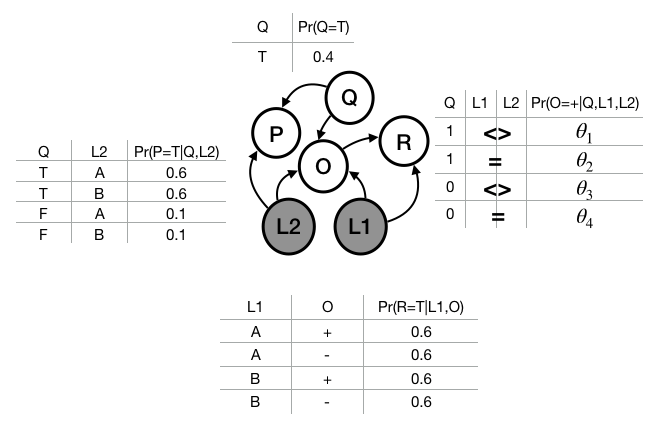
\includegraphics[width=\textwidth]{figs/BN.png}
  \end{minipage}\hfill
  \begin{minipage}[c]{0.45\textwidth}
    \caption{
        \small The model used for generating the datasets. There are four binary random variables, P, Q, O, and R. \textbf{P}: indicates whether or not the employee has high performance; \textbf{Q}: indicates whether or not an employee has high qualification; \textbf{O}: indicates whether or not the colleague submits the positive opinion towards the employee;  \textbf{R}: indicates whether or not the colleague has a positive opinion towards the employee;  \textbf{L1, L2}: indicates the label of the review provider and review receiver (observed).
    } \label{fig:BN}
  \end{minipage}
\end{figure}

We show the effectiveness of FairPSL by performing an empirical evaluation. We investigate two research questions in our experiments:
\begin{description}
\item[Q1] What is the effect of the fairness threshold $\delta$ on the fairness measures $RD/RC/RR$?
\item[Q2] How is decision quality affected by imposing $\delta$-fairness constraints?
\end{description}

Note that although we present the result for specific parameters of the framework in this section, we ran extensive analysis and the results we present are representative. We implemented the MAP inference routines of PSL and FairPSL in Python, using Gurobi-8.1\footnote{\url{www.gurobi.com}} as the backend solver. The FairPSL code, code for the data generator and data is publicly available\footnote{https://github.com/gfarnadi/FairPSL}. 

\subsection{Data generation}
  
We evaluate the FairPSL inference algorithm on synthetic datasets representing the performance review scenario (introduced in Example~\ref{ex:review}). The organization hierarchy is generated synthetically. 
The organization hierarchy generator is parameterized by two numbers: the number of employees in the organization ($n$) and the number of employees managed by each manager ($k$). Each employee is randomly assigned with a label \emph{A} or \emph{B}. An examples organization hierarchy with $n$=50 and $k$=3 is shown in Figure~\ref{fig:hierachy}.

\begin{figure}
  \begin{minipage}[c]{0.3\textwidth}
    \caption{
        \small An example of an organizational hierarchy with five levels and 50 employees with k=3. Each employee either has label A (shown with grey) or B (shown with white).
    }\label{fig:hierachy} 
	\end{minipage} \hfill
    \begin{minipage}[c]{0.7\textwidth}
    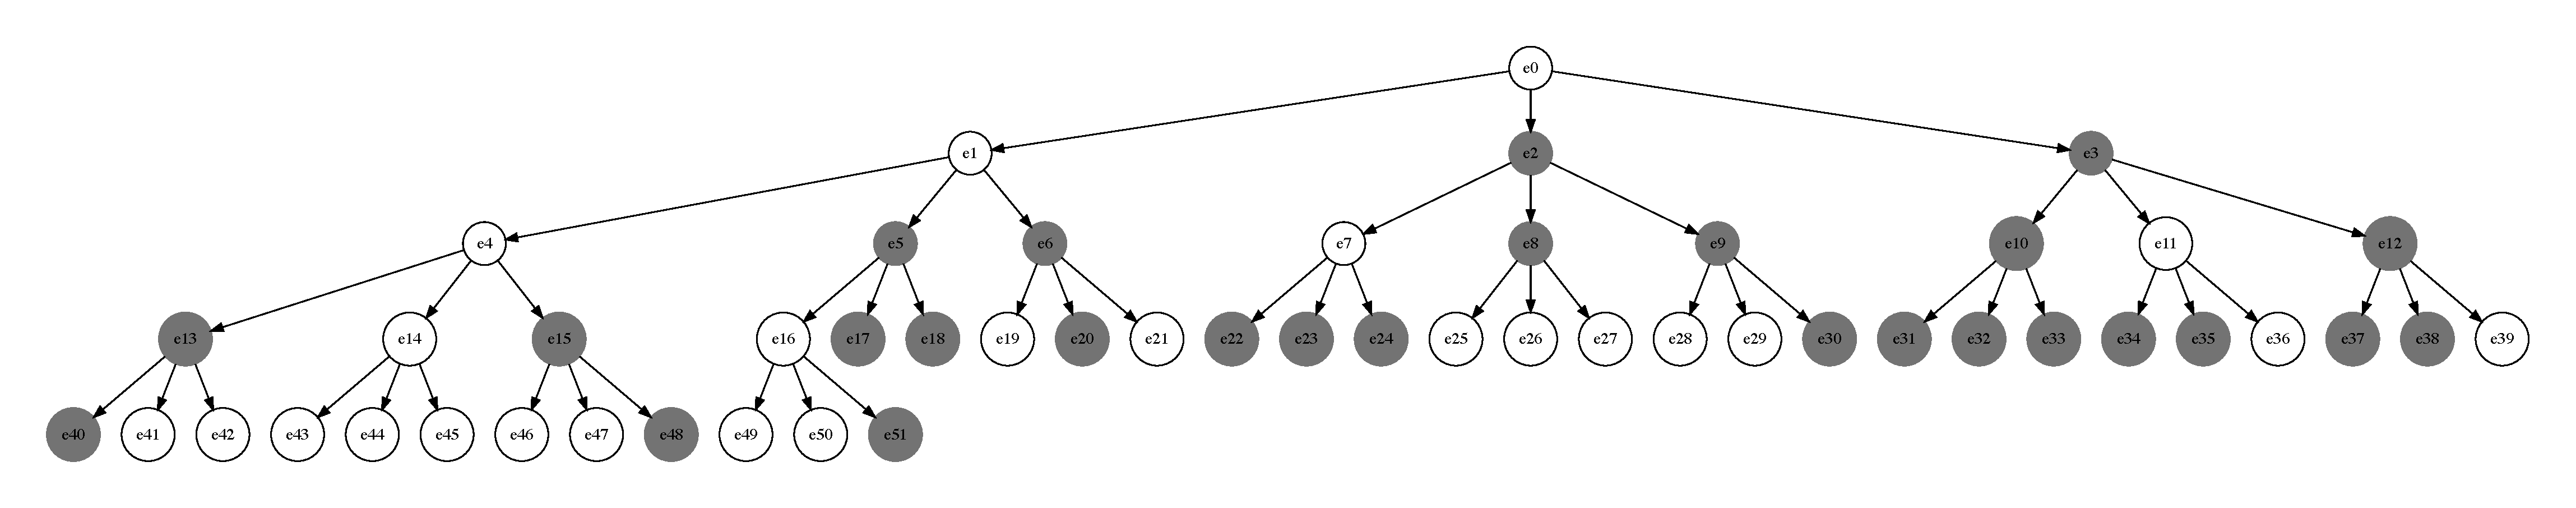
\includegraphics[width=\textwidth]{figs/Uni-hierachy.pdf}
  \end{minipage}
\end{figure}

For each employee, we use the generative model of Figure~\ref{fig:BN} to draw assignments for all the random variables. We assume that only $40\%$ of employees are qualified for promotion and regardless of their labels, employees submit only $60\%$ of their opinions. In addition, due to various personal and environmental factors, only $60\%$ of high quality employees perform well while $10\%$ of low quality employees also perform well regardless of their labels. Note that these numbers are not specific and just chosen for the framework to serve as a representative setting and a proof of concept. The conditional probability table for the opinion variable $O$ is parameterized by four values $(\theta_1, \theta_2, \theta_3, \theta_4)$ which together determine the degree of discrimination against the protected group. Since other parameters in the Bayesian network did not have a direct effect on the degree of discrimination, we fixed them to arbitrary values. 

The results presented in this section are based on an organization hierarchy  with $100$ employees where $k=5$. However, the results of the framework are not sensitive to the settings as we test the framework with various organization sizes ranging from $50$ to $500$ employees and various degree for $k$ ranging from $3$ to $10$. We generated seven datasets given the organization hierarchy using different values for the $\theta$ parameters: $(0.0,1.0,0.0,0.0)$, $(0.33,1.0,0.0,0.0)$, $(0.66,1.0,0.0,0.0)$, $(1.0,1.0,0.0,0.0)$, $(1.0,1.0,0.0,0.33)$, $(1.0,1.0,0.0,0.66)$, $(1.0,1.0,0.0,1.0)$. 
 
In the first three settings the discrimination originates from negative opinions towards qualified outgroup employees. The first setup is an extreme case where the opinion towards outgroup employees is always negative. The discrimination in the last three settings originates from positive opinions towards unqualified ingroup employees. The last setup is an extreme case where the opinion towards ingroup employees is always positive. The fourth setup represent unbiased opinions where employees are treated similarly based on their qualification. 

\paragraph{MAP Inference} We use the model presented in Table~\ref{tab:pslmodel} for MAP inference in PSL and FairPSL (recall that in FairPSL, the $\delta$-fairness constraints corresponding to one of the fairness measures are also added to the model). The observed atoms are $\textit{Manager(m,e)}$, $\textit{PositiveReview(e1,e2)}$ and labels of all employees. The truth values for all other atoms are obtained via MAP inference. We use the truth values obtained for the decision atoms $\textit{ToPromote(e)}$ to compute the fairness measures. We defined the discriminative pattern, and the protected and unprotected groups of this problem in Section~\ref{sec:formulation}.


\subsection{Evaluation results}

\begin{figure}
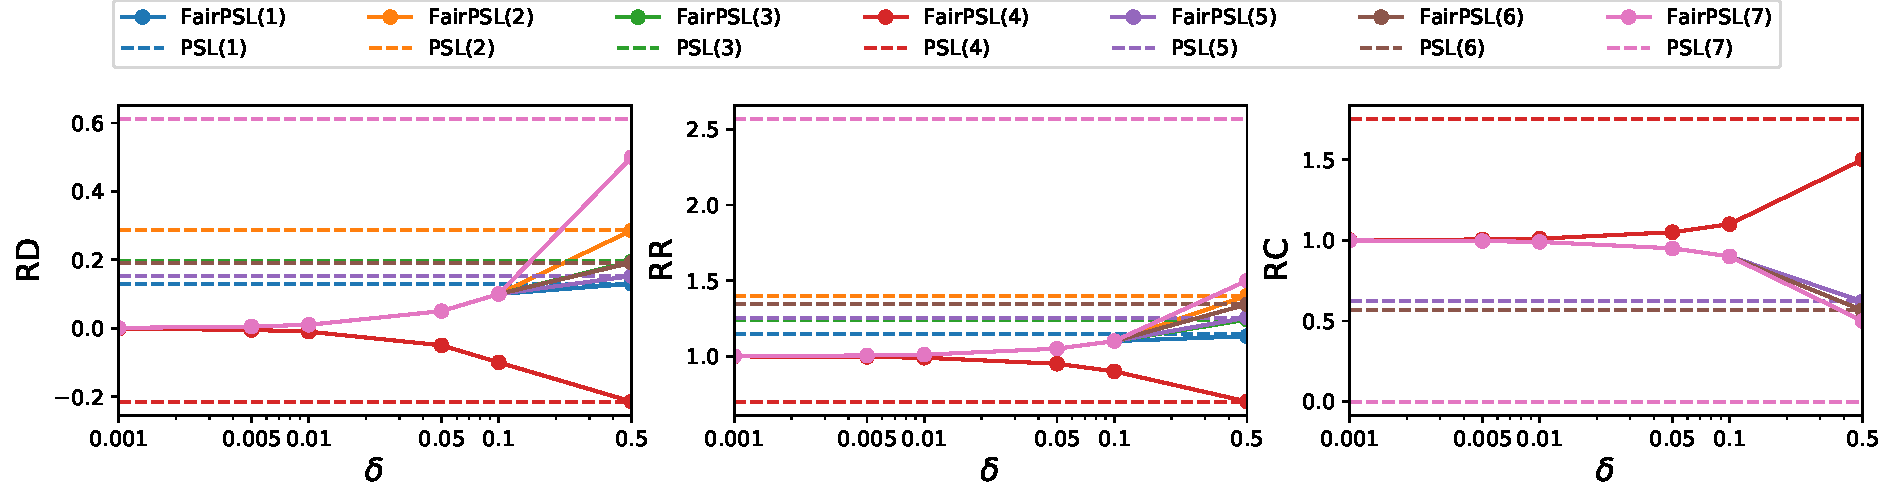
\includegraphics[width=1\linewidth]{figs/results_vis_uni_params.pdf}
\caption{\small Fairness score of predictions obtained by MAP inference of PSL and FairPSL, according to the fairness measures \emph{RD}, \emph{RR}, and \emph{RC}. The labels of datasets are mentioned with parenthesis next to the inference method. The FairPSL values of each measure are obtained by adding the $\delta$-fairness constraint of that measure.\label{fig:results}
}  
\end{figure}

To answer \textbf{Q1}, we run the MAP inference algorithm of PSL and FairPSL on seven synthetic datasets. 
We run the MAP inference of FairPSL multiple times on each dataset: For each of the three fairness measures, we add the corresponding $\delta$-fairness constraint with five thresholds $\{0.001, 0.005, 0.01, 0.05, 0.1, 0.5\}$.

Figure~\ref{fig:results} shows the fairness score of predictions in terms of the three fairness measures. As expected, tighter $\delta$-fairness constraints lead to better scores. Note that the best possible score according to RD is 0, as it computes a difference. Since RR and RC compute ratios, the best possible score according to these measures is 1. In our experiments, with any of these measures, taking $\delta = 0.001$ pushes the score of predictions to its limit.  

The $\delta$-fairness constraints modify the optimization problem of MAP inference by reducing the feasible region to solutions that conform with fairness guarantees. Research question \textbf{Q2} is concerned with the effect of this reduction on the accuracy of predictions. Note that decision quality is the same as the accuracy of predictions. To answer this question, we compare the inferred values for the decision atoms \textit{ToPromote(e)} against their actual values. These values are extracted from the known values of \textit{IsQualified(e)} according to rules 11 and 12 in Table~\ref{tab:pslmodel}. Figure~\ref{fig:accuracy} shows the area under the curve of the receiver operating characteristic~(AUC) of predicting the decision variable in three groups, namely the protected group, the unprotected group (i.e., promotion of the employees who have in-group managers), and all employees. By doing so, we make sure that our fairness constraints do not propagate bias towards either of the populations. Since the results of FairPSL with $\delta$-fairness constraints RR and RC are very similar to the results of RD, we only report the latter here.


\begin{figure}
    \centering
    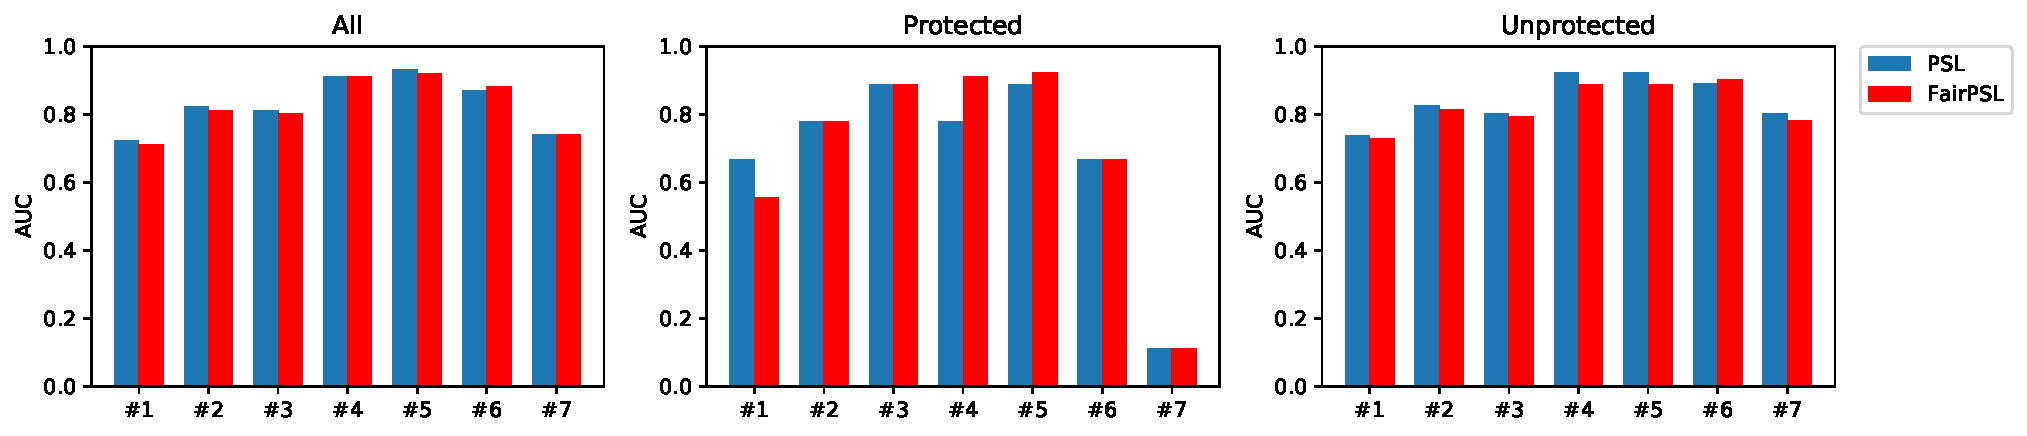
\includegraphics[width=\textwidth]{figs/roc.pdf}
    \caption{\small AUC score of predictions for truth values of unknown atoms \textit{ToPromote(e)} using MAP inference of PSL and FairPSL with $\delta$-fairness constraints $RD$ with $\delta=0.001$.}
    \label{fig:accuracy}
\end{figure}

According to Figure~\ref{fig:accuracy}, the results of both PSL and FairPSL in all seven datasets are close to each other. Note that although fairness may impose a cost in terms of overall accuracy, FairPSL often improves the accuracy of the protected class. Sometimes the overall predictions of FairPSL are even slightly better than PSL (e.g., dataset 6 and 7). As expected, the accuracy of the fourth setting where the opinions are unbiased are similar in both PSL and FairPSL. We observe that prediction of MAP inference for both FairPSL and PSL are similar, thus, in these settings at least, FairPSL guarantees fairness without hurting accuracy. Further investigation is required on the effect of the various ranges of discrimination (i.e., $\theta_1$, $\theta_2$, $\theta_3$, $\theta_4$) on the prediction results of FairPSL.



We also generate various types of organizations in which labels are not uniformly distributed, e.g., one population only occurs at the bottom levels of an organization. While we did not observe any differences in the behavior of our method with respect to accuracy and fairness measure, we found that the degree of discrimination is higher in such organizations. Further investigations on the structure of an organization on discrimination is an interesting direction for future research. 

\section{Conclusion and Future Directions}
\label{sec:conclusion}
Many applications of AI and machine learning affect peoples' lives in important ways. While there is a growing body of work on fairness in AI and ML, it assumes an individualistic notion of fairness.   In this paper, we have proposed a general framework for relational fairness which includes both a rich language for defining discrimination patterns and an efficient algorithm for performing inference subject to fairness constraints. We show our approach enforces fairness guarantees while preserving the accuracy of the predictions. 

There are many avenues for expanding on this work. For example, here we assumed that the discriminative pattern is given, however an automatic mechanism to extract discriminatory situations hidden in a large amount of decision records is an important and required task. Discrimination discovery has been studied for attribute-based fairness~\cite{pedreschi2013discovery}. An interesting next step is discrimination pattern discovery in relational data.

\section*{Acknowledgements}
This work is supported by the National Science Foundation under Grant Numbers CCF-1740850 and IIS-1703331. Golnoosh Farnadi and Behrouz Babaki are  supported by postdoctoral scholarships from IVADO through the Canada First Research Excellence Fund (CFREF) grant.

\begin{thebibliography}{10}
\itemsep=1pt 
\begin{small}

\bibitem{EUlaw}
European union legislation. (a) racial equality directive, 2000; (b) employment
  equality directive, 2000; (c) gender employment directive, 2006; (d) equal
  treatment directive (proposal), 2008.

\bibitem{UKlaw}
{UK} legislation. (a) sex discrimination act, 1975, (b) race relation act,
  1976.

\bibitem{USlaw}
United nations legislation. (a) universal declaration of human rights, 1948,
  (c) convention on the elimination of all forms of racial discrimination,
  1966, (d) convention on the elimination of all forms of discrimination
  against women, 1979.

\bibitem{alshukaili:iswc16}
Duhai Alshukaili, Alvaro A.~A. Fernandes, and Norman~W. Paton.
\newblock Structuring linked data search results using probabilistic soft
  logic.
\newblock In {\em International Semantic Web Conference {(1)}}, volume 9981 of
  {\em Lecture Notes in Computer Science}, pages 3--19, 2016.

\bibitem{bach:jmlr17}
Stephen~H. Bach, Matthias Broecheler, Bert Huang, and Lise Getoor.
\newblock Hinge-loss markov random fields and probabilistic soft logic.
\newblock {\em Journal of Machine Learning Research}, 18:109:1--109:67, 2017.

\bibitem{barocas2016big2}
Solon Barocas and Andrew~D Selbst.
\newblock Big data's disparate impact.
\newblock {\em California Law Review}, 104:671, 2016.

\bibitem{boyd2014networked}
Danah Boyd, Karen Levy, and Alice Marwick.
\newblock The networked nature of algorithmic discrimination.
\newblock In {\em Data and discrimination: Collected essays}, pages 53--57.
  2014.

\bibitem{brewer1979group}
Marilynn~B Brewer.
\newblock In-group bias in the minimal intergroup situation: A
  cognitive-motivational analysis.
\newblock {\em Psychological bulletin}, 86(2):307, 1979.

\bibitem{brewer2007social}
Marilynn~B Brewer.
\newblock The social psychology of intergroup relations: Social categorization,
  ingroup bias, and outgroup prejudice.
\newblock {\em Social Psychology: Handbook of Basic Principles}, 2007.

\bibitem{chouldechova2017fair2}
Alexandra Chouldechova.
\newblock Fair prediction with disparate impact: {A} study of bias in
  recidivism prediction instruments.
\newblock {\em CoRR}, abs/1703.00056, 2017.

\bibitem{dwork2012fairness3}
Cynthia Dwork, Moritz Hardt, Toniann Pitassi, Omer Reingold, and Richard~S.
  Zemel.
\newblock Fairness through awareness.
\newblock In {\em {ITCS}}, pages 214--226. {ACM}, 2012.

\bibitem{ebrahimi:emnlp16}
Javid Ebrahimi, Dejing Dou, and Daniel Lowd.
\newblock Weakly supervised tweet stance classification by relational
  bootstrapping.
\newblock In {\em {EMNLP}}, pages 1012--1017. The Association for Computational
  Linguistics, 2016.

\bibitem{farnadi2018fairness}
Golnoosh Farnadi, Behrouz Babaki, and Lise Getoor.
\newblock Fairness in relational domains.
\newblock In {\em AAAI/ACM Conference on AI, Ethics, and Society (AIES)}, pages
  108--114. ACM, 2018.

\bibitem{feldman2015certifying2}
Michael Feldman, Sorelle~A. Friedler, John Moeller, Carlos Scheidegger, and
  Suresh Venkatasubramanian.
\newblock Certifying and removing disparate impact.
\newblock In {\em {KDD}}, pages 259--268. {ACM}, 2015.

\bibitem{getoor2007introduction}
Lise Getoor and Ben Taskar.
\newblock {\em {Introduction to Statistical Relational Learning}}.
\newblock MIT press Cambridge, 2007.

\bibitem{hardt2016equality3}
Moritz Hardt, Eric Price, and Nati Srebro.
\newblock Equality of opportunity in supervised learning.
\newblock In {\em {NIPS}}, pages 3315--3323, 2016.

\bibitem{kamishima2011fairness}
Toshihiro Kamishima, Shotaro Akaho, and Jun Sakuma.
\newblock Fairness-aware learning through regularization approach.
\newblock In {\em ICDMW}, pages 643--650. {IEEE} Computer Society, 2011.

\bibitem{kouki:recsys15}
Pigi Kouki, Shobeir Fakhraei, James~R. Foulds, Magdalini Eirinaki, and Lise
  Getoor.
\newblock Hyper: {A} flexible and extensible probabilistic framework for hybrid
  recommender systems.
\newblock In {\em RecSys}, pages 99--106. {ACM}, 2015.

\bibitem{counterfactualfairness}
Matt~J. Kusner, Joshua~R. Loftus, Chris Russell, and Ricardo Silva.
\newblock Counterfactual fairness.
\newblock In {\em {NIPS}}, pages 4069--4079, 2017.

\bibitem{Pedreschi:2012}
Dino Pedreschi, Salvatore Ruggieri, and Franco Turini.
\newblock A study of top-k measures for discrimination discovery.
\newblock In {\em {SAC}}, pages 126--131. {ACM}, 2012.

\bibitem{pedreschi2013discovery}
Dino Pedreschi, Salvatore Ruggieri, and Franco Turini.
\newblock The discovery of discrimination.
\newblock In {\em Discrimination and Privacy in the Information Society},
  volume~3 of {\em Studies in Applied Philosophy, Epistemology and Rational
  Ethics}, pages 91--108. Springer, 2013.

\bibitem{ridgeway2004unpacking}
Cecilia~L Ridgeway and Shelley~J Correll.
\newblock Unpacking the gender system: A theoretical perspective on gender
  beliefs and social relations.
\newblock {\em Gender \& society}, 18(4):510--531, 2004.

\bibitem{sridhar:bioinformatics16}
Dhanya Sridhar, Shobeir Fakhraei, and Lise Getoor.
\newblock A probabilistic approach for collective similarity-based drug-drug
  interaction prediction.
\newblock {\em Bioinformatics}, 32(20):3175--3182, 2016.

\bibitem{verma2018fairness2}
Sahil Verma and Julia Rubin.
\newblock Fairness definitions explained.
\newblock In {\em 2018 IEEE/ACM International Workshop on Software Fairness
  (FairWare)}, pages 1--7. IEEE, 2018.

\bibitem{west2014exploiting}
Robert West, Hristo~S. Paskov, Jure Leskovec, and Christopher Potts.
\newblock Exploiting social network structure for person-to-person sentiment
  analysis.
\newblock {\em {TACL}}, 2:297--310, 2014.

\bibitem{zafar2017parity}
Muhammad~Bilal Zafar, Isabel Valera, Manuel Gomez{-}Rodriguez, Krishna~P.
  Gummadi, and Adrian Weller.
\newblock From parity to preference-based notions of fairness in
  classification.
\newblock In {\em {NIPS}}, pages 228--238, 2017.

\bibitem{zemel2013learning}
Richard~S. Zemel, Yu~Wu, Kevin Swersky, Toniann Pitassi, and Cynthia Dwork.
\newblock Learning fair representations.
\newblock In {\em {ICML} {(3)}}, volume~28 of {\em {JMLR} Workshop and
  Conference Proceedings}, pages 325--333. JMLR.org, 2013.

\end{small}
\end{thebibliography}

\end{document}

\end{article}

\makeatletter
\renewcommand{\AB@affillist}{}
\renewcommand{\AB@authlist}{}
\setcounter{authors}{0}
\makeatother

\begin{article}
{Advancing RPC for Data Services at Exascale}
{Jerome Soumagne, Philip Carns and Robert B. Ross}
\graphicspath{{submissions/jerome/}}
\documentclass[11pt]{article}

%\usepackage{deauthor}

%\usepackage{times}

%\usepackage[pdftex]{graphicx}
%\DeclareGraphicsExtensions{.pdf,.jpeg,.jpg,.png}
%\graphicspath{{soumagne/}}

%\usepackage[affil-it]{authblk}
%\setlength{\affilsep}{0em}

%\usepackage[labelfont=bf,labelsep=space,list=true]{subcaption}

%\usepackage{url}

\begin{document}
\title{Advancing RPC for Data Services at Exascale}
\author[1]{Jerome Soumagne}
\author[2]{Philip Carns}
\author[2]{Robert B. Ross}
\affil[1]{The HDF Group}
\affil[2]{Argonne National Laboratory}

\maketitle

\begin{abstract}
Remote Procedure Call (RPC) has long been an inherent component of parallel
file systems and I/O forwarding middleware in high-performance computing
(HPC).  RPCs are used in this environment to issue
I/O operations and transfer data from compute nodes to gateway and server storage
nodes. With HPC systems becoming more heterogeneous, data volumes
reaching new thresholds, and I/O standing as the main bottleneck, there is a growing
need in the HPC community to build distributed services and adopt new workflows
that are, nonetheless, no longer dictated by monolithic parallel file systems. These include
specialized storage, data analysis, and telemetry
services that can be adapted to fit application needs. Parallel file system
RPC facilities have never been exposed to service or middleware developers,
however, leaving them with two choices: MPI or the low-level fabric network
protocol.
In this article, we show how an independent RPC framework can be used as a building block for
developing user-level data services at exascale. We identify the design
choices that must be considered in terms of both performance and resilience
for HPC
data services, and we discuss the directions taken to palliate current HPC system constraints.
\end{abstract}

\section{Introduction}
\label{sec:intro}

High-performance computing (HPC) facilities have traditionally
been designed around \textit{monolithic} file systems, which are tailored to
scientific HPC workflows comprised of computation, storage, and
data analysis. Scientific application users, whose needs depend
on the application's domain, have been constrained to conform to system precepts
and this standard workflow. While this has been
a viable (but increasingly limiting) option for pre-exascale systems,
increasing data volumes and increasing system complexity with
emerging hardware are now forcing application users to adopt new
\textit{specialized} workflows.  These specialized workflows not only achieve sustainable
performance and perform data analysis in a timely manner at an increasing
scale, but also better respond to application needs and provide data
insights, for example through monitoring and telemetry service.

Creating specialized workflows requires the introduction of
a collection of \textit{data services} to the HPC ecosystem that must interact
with both the
system components (hardware and software) and the application.
While some of those services may be provided by the system, the vast majority
of data services are user-level services that are developed to augment the
original HPC system software stack and better serve the application's
performance or functionality needs. Data services (system-provided
or user-provided) must respond, in most cases, to the same user
prerequisites by ensuring performance, resilience, and ease of deployment.
These prerequisites introduce engineering challenges that
must be overcome when creating a new HPC data service---by no means an
easy task. One such challenge is communication: data exchange
between services is a critical aspect of
specialized workflows that are composed of multiple services interacting with
each other. Developing the messaging part of a data service component on an HPC
machine can, for a new service developer, involve either using the
low-level network fabric
API, which requires a significant amount of work and expertise, or using the vendor installed
MPI library~\cite{mpich} that takes advantage of the underlying network fabric. 
MPI itself, however, is not very suitable for developing such dynamical services that
may come and go
%, nor is it suitable for efficiently accessing memory of a remote process
%without prior collective synchronization
~\cite{Zounmevo2013}.
%
MPI implementations have consistently prioritized use
by applications and not by service libraries.

Data services are already a well-established technology in the cloud, where
remote procedure call (RPC) is the main technique used for sending messages
to remote components. Google gRPC~\cite{protobuf} or Facebook Thrift~\cite{Slee2007}
are good examples of such
frameworks. However, they are not well-suited to run on HPC systems because they (1)
rely on the TCP/IP stack and do not take advantage of the low latency/high
bandwidth HPC fabrics and (2) are not designed for exchanging very large amounts
of data, a task that is left to the user.
In contrast, RPC has been used as the communication pillar of
distributed file systems (e.g., Lustre Networking (LNET)~\cite{Wang2009},
Panasas~\cite{Welch2008}) and I/O forwarding layers
(e.g., IOFSL~\cite{Ali2009}) that are specifically designed to send I/O requests on top of the
underlying network fabric. The Network File System (NFS)~\cite{Sandberg1988}
is also a good example of the use of RPC with large data transfers and
therefore close to the use of RPC in an HPC system.
The internal RPC facilities of these file systems (with the exception of NFS) have,
nonetheless, never
been directly exposed to users; instead, they have been deeply buried in the
monolithic file system software stacks that often extend into kernel space.
Other parallel file systems have implemented their own network abstraction layer
to support multiple network fabrics
and provide messaging capabilities that can support data services. However, they are not
general-purpose RPC frameworks, and in most cases cannot be easily extracted
from the file systems that they were designed for.

Based on both of those technologies and past experience with I/O forwarding,
we introduced in~\cite{Soumagne2013} an RPC framework, called Mercury, that takes
advantage of low-level HPC network fabrics and facilitates the development
of user-level data services. Mercury is part of a more comprehensive suite of components named
Mochi~\cite{Ross2020} that provides
a collection of service components for the creation of specialized data services.
We present in this paper how some of the design
choices made for Mercury are essential for building an heterogeneous service
workflow in an exascale HPC environment. In Section~\ref{sec:related}, we
present some of the work that
is similar to Mercury and approaches that we take to develop user-level data
services. In Section~\ref{sec:overview}, we give a brief overview of Mercury's
architecture before focusing in Section~\ref{sec:design} on the specific design
points that make an RPC framework usable for HPC data services, supporting our
claims by evaluation results. In Section~\ref{sec:apps}, we present some of the data services that are
successfully being deployed using Mochi and Mercury.
In Section~\ref{sec:concl}, we summarize our conclusions.

\section{Related Work}
\label{sec:related}

A few other frameworks and suites of HPC data service components have been proposed
using an approach similar to the one we used in Mercury. We present here
three of the most notable frameworks.

\textit{DataSpaces}~\cite{Docan2012} implements a
scalable, semantically specialized shared-space abstraction that is
dynamically accessible by all components and services in an application
workflow, supporting both application/system-aware data placement and data movement.
It relies on the \textit{Decoupled and Asynchronous Remote Transfers} (DART)~\cite{Docan2010}
layer, which is not defined as an explicit RPC framework, although it allows transfer of
large amounts of data using a client/server model from applications running on
the compute nodes of an HPC system to local storage or remote locations, in
order to enable remote application monitoring, data analysis, code coupling,
and data archiving.
The key requirements that DART seeks to satisfy are minimizing data transfer
overheads on the application; achieving high throughput, low latency data
transfers; and preventing data losses. To this end, DART is
designed so that dedicated nodes (i.e., separate from the application compute
nodes) asynchronously extract data from the memory of the compute nodes using
remote direct memory access (RDMA).

The \textit{Scalable Observation System} (SOSflow)~\cite{Wood2016} provides a broad
set of online and in situ capabilities, including code steering via remote method
invocation, data analysis, and visualization. SOSflow can couple together
multiple sources of data, such as application components and operating
environment measures, with multiple software libraries and performance
tools. SOSflow's communication mechanism relies both on TCP sockets for
on-node communication and on MPI for off-node communication. Its main communication
pattern is a publish-and-subscribe mechanism and relies on a daemon that is
launched as a background  process  in  user space at the start of a
job script, before the scientific workflow begins.

\textit{Faodel}~\cite{Ulmer2018} provides a set of services for data
management and exchange in HPC workflows. Three major components of
Faodel are Kelpie, Opbox, and Lunasa. Kelpie provides a key-blob
abstraction. OpBox is a library for implementing asynchronous communication
between multiple entities in a distributed application, and provides the user
with primitives for expressing a protocol as a state machine that the
communication layer can process in an asynchronous manner. It also provides
a naming service to locate components of an application. Lunasa provides
user-level network memory management services and effectively
acts as a memory registration cache for doing RDMA. Faodel relies on
an evolution of the NNTI layer from the \textit{NEtwork Scalable
Service Interface} (Nessie)~\cite{Lofstead2011} RPC library.
It provides an asynchronous RPC solution, designed to overlap computation and
I/O. Nessie also provides a mechanism to handle bulk data transfers, which can use
RDMA to transfer data efficiently from one memory to the other, and supports
several network transports. Nessie uses the RPC interface to push
control messages to the servers and exposes a separate one-sided API that is
used to push or pull data between client and server.

\section{Overview and Considerations}
\label{sec:overview}

Mercury is designed around three key paradigms: provide reliable RPC
functionality, support large data arguments, and take advantage of the HPC network
fabrics. In terms of functionality, much more is needed when
developing distributed HPC data services; but as opposed to RPC frameworks that are
part of monolithic software stacks, Mercury remains as thin as possible
in order to allow for reusability between various service components that must
support different needs.

\begin{figure}[h]
\centering
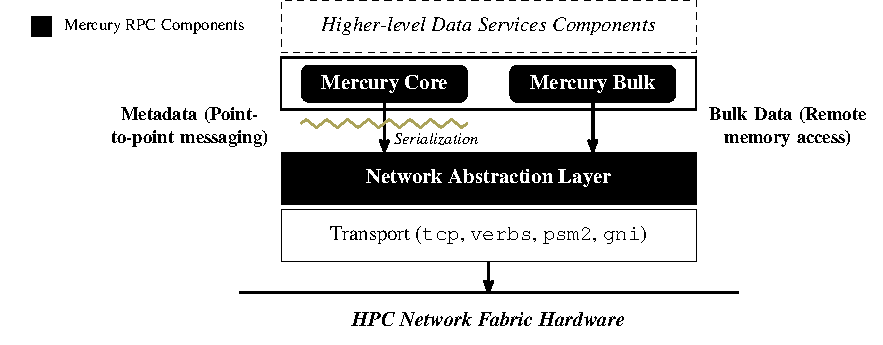
\includegraphics{figs/overview}
%\vspace{-5pt}
\caption{Overview of Mercury RPC components in the software stack.}
\label{fig:overview}
%\vspace{-10pt}
\end{figure}

As shown in Figure~\ref{fig:overview}, Mercury is composed of
two service-level components:
a core RPC component, which is designed to serialize
function arguments and send them to a remote target for execution using
point-to-point messaging, and a bulk
component, which is designed to handle large arguments (i.e., arguments that are
generally larger than 4KB depending on the underlying protocol being used).
This latter component enables the creation of
memory descriptors that can be sent along with the other arguments to the RPC
target to initiate raw memory transfers (without serialization) using remote memory access (RMA).
In Section~\ref{sec:rdma}, we detail this scenario and its benefits.
%
In order to support a large variety of HPC network fabrics,
both of these components interface with a network abstraction
layer that provides a minimum set of network primitives for both
point-to-point messaging and one-sided RMA communication operations.
Moreover, in order to reduce the burden of connection handshakes
when the underlying network does not necessarily request it (also
essential for scalability) and to support services that may come and go,
remote peers are addressed through unconnected endpoints.
Furthermore, in order to maximize throughput, all communication is made
nonblocking through a callback-based approach that we detail in
Section~\ref{sec:cb}.

While these points describe the overall architecture of an RPC
framework for HPC, additional key items can rapidly become prerequisites for
creating an RPC framework that is designed to support data services. These
include maximizing throughput, providing scaling, 
enabling flexibility, and ensuring resilience. In the
following section we describe how one can enhance RPC to (1) leverage RDMA-capable networks;
(2) support node-local service scaling and leverage multi-core processors;
(3) enable flexible, node-local deployment scenarios and service 
composition; (4) bridge nodes between multiple HPC networks; (5) enable fault tolerance.

\section{Enabling RPC for HPC Data Services}
\label{sec:design}

We do not compile an exhaustive list of features in this section.
%
Instead, we focus on those features that are necessary to enable strong service scaling,
performance, flexibility, and resilience for data services on emerging
large-scale computing platforms.

\subsection{HPC Network Support}
\label{sec:rdma}

As opposed to cloud-based RPC solutions that rely on TCP networking,
HPC network fabrics provide dedicated solutions that offer both
low latency and high bandwidth. To take advantage of these solutions, however, 
an RPC framework must leverage low-level vendor APIs such as InfiniBand{\small \texttrademark} Verbs,
Intel{\textsuperscript{\textregistered}} Performance Scaled Messaging 2 (PSM2),
and Cray{\textsuperscript{\textregistered}} Generic Network Interface (GNI).
Rather than implementing Mercury's network
abstraction layer directly on top of those APIs, we currently use
OFI libfabric~\cite{Grun2015} as
the intermediate layer that abstracts RDMA capabilities for RDMA-capable
networks or emulated RMA (over point-to-point) for noncapable networks.
Exposing native RDMA primitives is essential for taking full advantage of RDMA
capable networks so that a data service can, for large data, leverage zero-copy
transfers from the application's memory from/to the storage.

\begin{figure}[h]
\centering
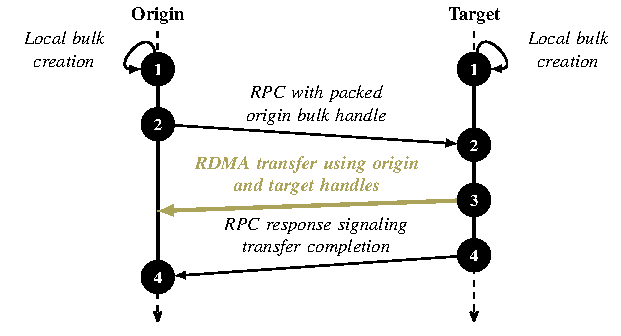
\includegraphics{figs/bulk_rdma}
\vspace{-5pt}
\caption{Four-step process of Mercury's bulk RDMA transfers.}
\label{fig:bulk_rdma}
\vspace{-10pt}
\end{figure}

Enabling RMA capabilities through Mercury's bulk component (see Figure~\ref{fig:overview})
is a four-step process (see Figure~\ref{fig:bulk_rdma}).
First, \textit{bulk handles}, which are abstract memory
descriptors, must be created on both origin and target processes. During
handle creation, memory regions are registered (which in most cases
corresponds to a physical hardware registration); this allows for the
higher level data service to only expose memory pages that it wishes to access in either
read-write or read-only mode. Second, an RPC is issued from the origin
process to the target process with the serialized bulk handle of the origin process;
this handshake allows the target process to gather virtual address information,
registration keys, and so forth, which are necessary for the underlying protocol to post
an RDMA operation.
Third, the actual RDMA operation is posted using both the target's local bulk handle
and the origin's handle that was transmitted through the RPC. Since bulk handles are
abstract memory descriptors, more complex scenarios such as scatter/gather can
be transparently implemented and even delegated to the hardware if the hardware provides this support,
allowing for more efficient transfers. Finally, the RPC response is sent, effectively 
signaling the origin of the transfer completion. This server-driven four-step process is
the most conventional model for data transfers in Mercury, but client-driven transfers are legal
as well. The former is
more commonly recommended for two reasons. First, it enables servers to throttle or
re-order
transfers according to load.  Second, it makes the clients lighter weight and more scalable,
since they do not have to track the state of server resources.

\paragraph{Evaluation.}
To show the importance of supporting this capability, we compare the RPC performance and ``RPC with bulk'' performance
on an InfiniBand cluster (Cooley) that is equipped with 4X FDR Infiniband cards (56 Gb/s).
Compared to TCP over the same network,
our approach improves RPC throughput with close to
$9\times10^{5}$ operations per second and close to 6,000 MB/s average throughput when performing RPC and bulk transfer through the native verbs interface.
Note that the previous results do not use any multi-threading capabilities. We maintain
a number of 32 RPCs in-flight to ensure sustained performance. Multi-threading support is
discussed in the next section.

\begin{figure*}[h]
\subfloat[RPC round-trip benchmark (32 RPCs in-flight).\label{fig:rpc_rate_verbs}]{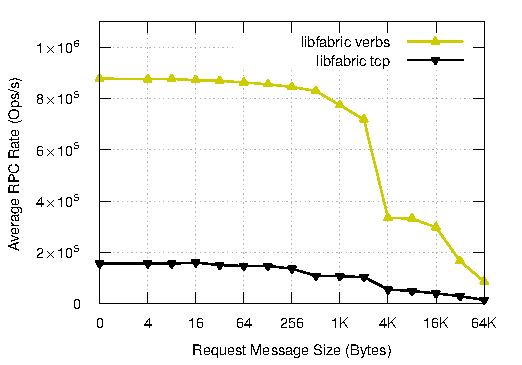
\includegraphics[width=0.49\linewidth]{figs/rpc_rate_verbs} }
\subfloat[Bulk transfer (server pull) benchmark (32 RPC in-flight).\label{fig:write_bw_verbs}]{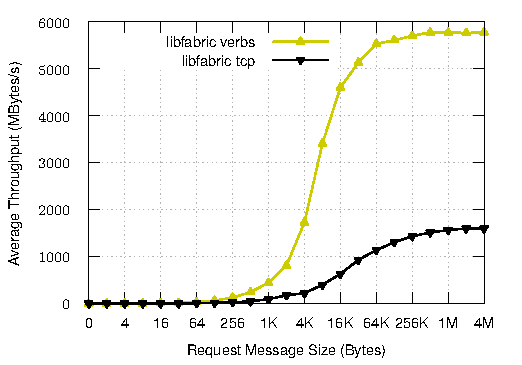
\includegraphics[width=0.49\linewidth]{figs/write_bw_verbs} }
\caption{Effect of leveraging RDMA network on InfiniBand cluster (FDR InfiniBand).}
\label{fig:bench_verbs}
\end{figure*}

\subsection{Multi-Core Architecture Support}
\label{sec:local_scaling}

With CPUs experiencing increasing core count and lower frequencies per
core, data services are expected to take advantage of these architectures
by either distributing the load of incoming RPCs across cores or by
running multiple services co-located within the same node.
% One of the points that we have not detailed so far is Mercury's progress model.
%
Communication
frameworks typically adopt one of two progress models: either \textit{explicit} or
\textit{implicit}. \textit{Explicit} progress implies that the user will regularly
make progress calls to effectively check into network completion queues, poll
file descriptors, etc. In contrast, an \textit{implicit} progress model will 
make progress in background without any need for the user to be involved.
However, this usually involves a background progress thread 
running to make progress while operations are being posted. While
this may seem convenient, this ``hidden'' thread can become detrimental when
running concurrently with other user's threads, leading to unexpected scheduling
issues.
%
Therefore, to prevent this type of issues and give data services sufficient
flexibility in how progress is ensured, we follow an explicit progress
model.
%
RPC is not only about messaging and communication, it is also about
execution of user-defined function calls. When making progress, therefore, it is
often desirable to decouple the RPC execution activities from the network progress activities,
which leads us to actually adopt a \textit{progress-and-trigger} model
that gives services more control over the placement of the progress and
execution threads.
%
In this approach, implicit progress can be accomplished
by the user by having a thread calling progress in background. 

In a typical scenario, an RPC listener service will start posting RPC receive
operations with memory bound to the thread posting the operations.
%
Distributing the execution of these incoming RPCs across multiple threads
(e.g., using a thread pool) can lead to several context switches
at a significant performance penalty. To prevent this scenario, take
advantage of multi-core architectures, and allow for node-local service scaling
without costly creation of separate endpoints per thread, we make
use of \textit{scalable endpoints} (SEP) when available.
%
Scalable endpoints are provided through libfabric~\cite{Grun2015} but
can be extended through our network abstraction layer.
Scalable endpoints allow for
sharing a single endpoint resources between threads by assigning separate
transmit and receive contexts (including completion queues) to each thread. When SEPs
are used, context switches between threads no longer exist---
a fundamental advantage for RPC multi-core architectures.


\begin{figure*}[h]
\subfloat[RPC round-trip benchmark (32 RPCs in-flight).\label{fig:rpc_sep_gni}]{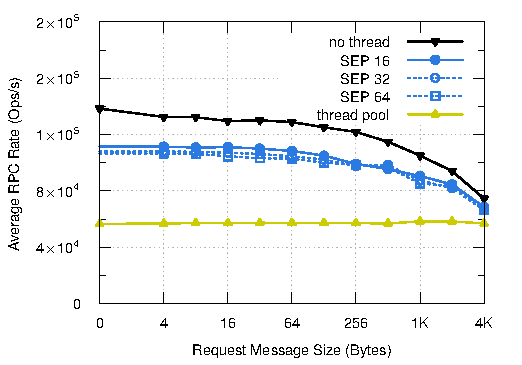
\includegraphics[width=0.49\linewidth]{figs/rpc_rate_sep_gni} }
\subfloat[Bulk transfer benchmark (32 RPC in-flight).\label{fig:write_bw_sep_gni}]{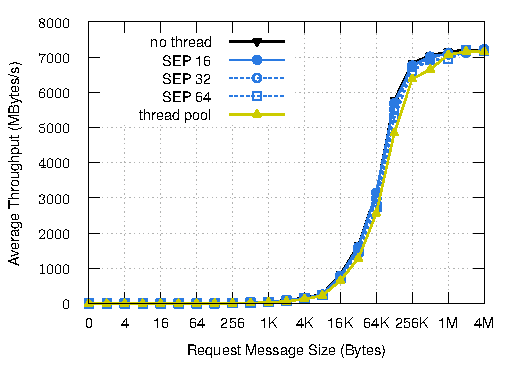
\includegraphics[width=0.49\linewidth]{figs/write_bw_sep_gni} }
\caption{Effect of using scalable endpoints on Cray XC40 (Aries interconnect).}
\label{fig:bench_sep_gni}
\end{figure*}

%\begin{figure*}[h]
%\begin{subfigure}[b]{.49\linewidth}
%\centering
%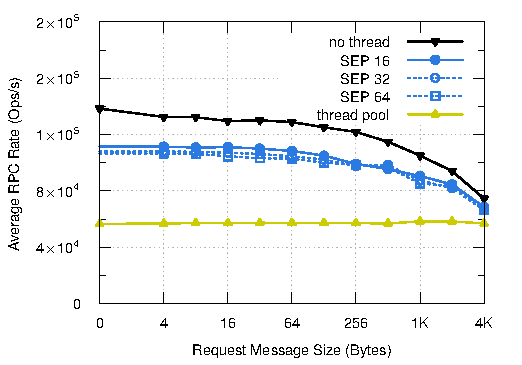
\includegraphics[width=\textwidth]{figs/rpc_rate_sep_gni}
%\caption{RPC round-trip benchmark (32 RPCs in-flight).}
%\label{fig:rpc_rate_sep_gni}
%\end{subfigure}%
%\hfill
%\begin{subfigure}[b]{.49\linewidth}
%\centering
%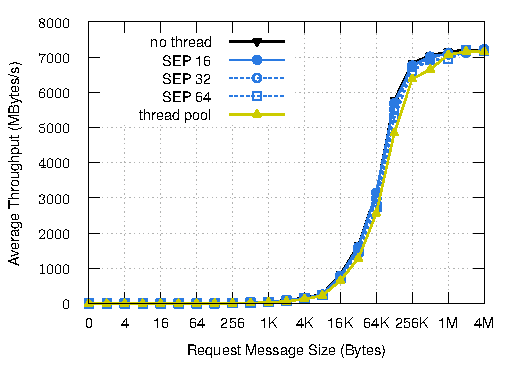
\includegraphics[width=\textwidth]{figs/write_bw_sep_gni}
%\caption{Bulk transfer benchmark (32 RPCs in-flight).}
%\label{fig:write_bw_sep_gni}
%\end{subfigure}
%\vspace{-5pt}
%\caption{Effect of using scalable endpoints on Cray XC40 (Aries interconnect).}
%\label{fig:bench_sep_gni}
%\vspace{-15pt}
%\end{figure*}

\paragraph{Evaluation.} To demonstrate the impact of context switches
and emphasize the benefits of scalable endpoints, we run two
benchmarks on the Theta supercomputer at the Argonne Leadership Computing Facility (ALCF).
Theta is a Cray XC40 system with a second-generation Intel Xeon Phi processor and
Cray Aries interconnect. Each compute node is a single Xeon Phi chip with 64 cores,
16 GB of Multi-Channel DRAM (MCDRAM), and 192 GB of DDR4 memory.
Users typically take advantage of this architecture by either deploying
multiple data services locally or by distributing incoming RPCs across cores.
%
In order to do so using SEP, we assign each core
to make progress and trigger calls on their own receive context.
As shown in Figure~\ref{fig:bench_sep_gni}, using SEP provides
close match (in terms of operations per second) to the performance of workloads
that do not use multi-threading. 
%
Distributing requests using a thread pool, in contrast, has a significant
detrimental impact on RPC rate.  Note that in all cases bulk transfers
exhibit similar overall bandwidth, as context switches only represent a
portion of the time spent when large data is transferred over the network.

\subsection{Flexible Provisioning and Topology}
\label{sec:local_deployment}

In the preceding section, we demonstrated node-level scaling when RPCs are made between
separate nodes using the native interconnect. Additional optimization can be made,
however, by being aware of node-local process placement, in order to ensure efficient
composition of services.

\subsubsection{Transparent Node-Local Deployment}

When deploying data
services, it is common for some of these services to either issue
RPCs to other local services (i.e., separate processes within the same node) or
to send RPCs back to themselves (i.e., within the same process).
The latter typically arises out of convenience, rather than creating a separate code path for
that case.
To achieve the former,
Mercury can make use of shared-memory transparently by detecting that
the target address is on the same node. Using lockless shared ring buffers and
lockless queues, it is possible to achieve lockless transfers with very low
latency. For bulk data transfers and to prevent any intermediate \textit{memcpy},
zero-copy transfers (i.e, one single and direct copy from origin to target buffer) can be
achieved using the Linux Cross-Memory Attach mechanism.

To achieve the latter, Mercury detects when the target address is the
same as the origin address and sends RPCs using the same argument packing mechanism,
by immediately queuing the RPC into a local completion queue, internally signaling
completion to wake up any potential thread waiting in a progress call. Likewise,
bulk data transfers are realized through a \textit{memcpy} between source and
destination buffers.

This combination of transparent shared-memory transfers between separate processes,
loopback redirection within the same process, and over-the-wire transfers has
shown substantial benefits when deploying data services in terms of performance
and flexibility, since data services can treat all three scenarios identically.


\begin{figure*}[h]
\subfloat[RPC round-trip benchmark (32 RPCs in-flight).\label{fig:rpc_rate_sm}]{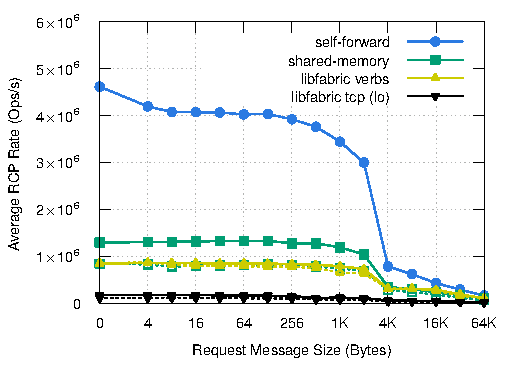
\includegraphics[width=0.49\linewidth]{figs/rpc_rate_sm} }
\subfloat[Bulk transfer benchmark (32 RPC in-flight).\label{fig:write_bw_sm}]{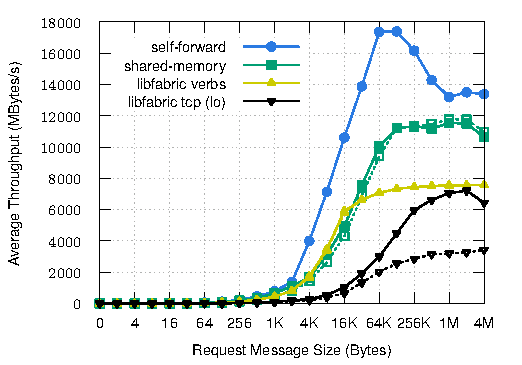
\includegraphics[width=0.49\linewidth]{figs/write_bw_sm} }
\caption{Comparison between node-local RPC mechanisms on InfiniBand cluster (FDR InfiniBand).}
\label{fig:bench_sm}
\end{figure*}

%\begin{figure*}[h]
%\begin{subfigure}[b]{.5\linewidth}
%\centering
%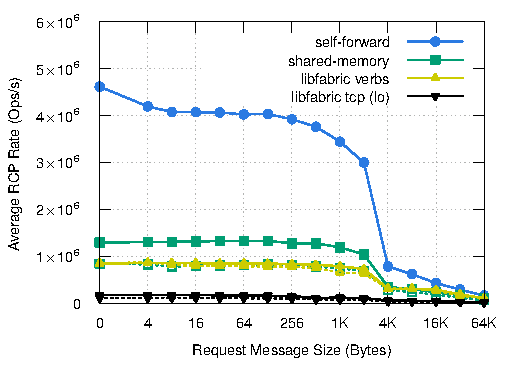
\includegraphics[width=\textwidth]{figs/rpc_rate_sm}
%\caption{RPC round-trip benchmark (32 RPCs in-flight).}
%\label{fig:rpc_rate_sm}
%\end{subfigure}%
%\hfill
%\begin{subfigure}[b]{.5\linewidth}
%\centering
%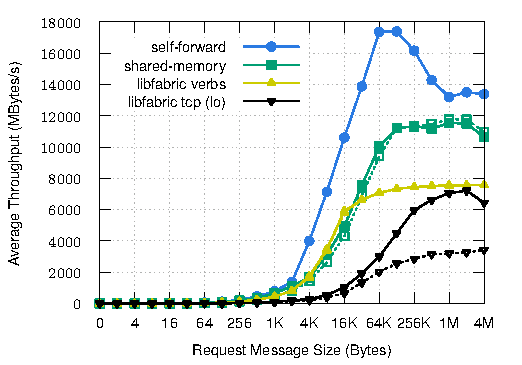
\includegraphics[width=\textwidth]{figs/write_bw_sm}
%\caption{Bulk transfer (server pull) benchmark (32 RPCs in-flight).}
%\label{fig:write_bw_sm}
%\end{subfigure}
%\vspace{-5pt}
%\caption{Comparison between node-local RPC mechanisms on InfiniBand cluster (FDR InfiniBand).}
%\label{fig:bench_sm}
%\vspace{-10pt}
%\end{figure*}

\paragraph{Evaluation.} To illustrate this scenario on our InfiniBand cluster (Cooley),
we compare in  Figure~\ref{fig:bench_sm} our two local RPC communication mechanisms 
to issuing RPCs either through the native interconnect (in this case InfiniBand Verbs)
or through TCP and the loopback interface. The latter is one of the fallback 
mechanisms typically used when not using shared-memory.
Cooley is equipped of dual-sockets nodes with Intel Xeon E5-2620 v3 CPUs. Consequently,
performance varies depending on process placement and the NUMA nodes being used---performance when running on separate NUMA nodes is represented by a dotted line in Figure~\ref{fig:bench_sm}.
In terms of both RPC
operations per second and bulk throughput, these two mechanisms are very valuable,
providing much better performance than both the native interconnect and TCP
(1.3 MOps/s for shared-memory and more than 4 MOps/s for loopback execution).
When running on separate NUMA nodes, shared-memory performance is naturally
impacted, though RPCs with bulk transfer still perform at a much higher rate due to the use
of Linux Cross-Memory Attach (CMA).

\subsubsection{Service Composition}

With node-level scaling and transparent node-local deployment in place,
composing data services seems the next natural step. In order to provide flexible composition, 
the RPC API must not be specific to any implementation but rather rely only on \textit{origin} and
\textit{target} concepts. The RPC mechanism then can be consistently employed to communicate
between different service ``servers'' and ``clients''.

\begin{figure}[h]
\centering
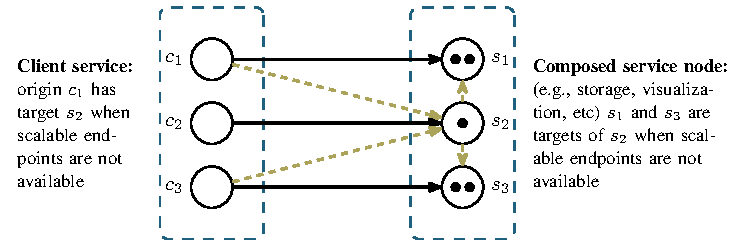
\includegraphics{figs/composition}
\caption{Composition of services with and without scalable endpoints.}
\label{fig:composition}
%\vspace{-5pt}
\end{figure}

When multiple services are colocated, there is also a need for addressing specific services and 
efficiently making progress. 
%
As shown in Figure~\ref{fig:composition}, this can then be accomplished by
using a ``delegator'' service, which can potentially become a bottleneck,
or by using scalable endpoints addressing specific receive contexts
directly through an ID that can be defined for each data service.
%
When there is no hardware support for scalable endpoints, however, this
functionality must be emulated by embedding a service ID into the RPC
header and using that ID to distribute RPC requests to the corresponding
service through that delegator.  An alternative is to create multiple
endpoints, one for each data service; but this is usually not recommended
due to hardware resource limitations.

\subsection{Multi-Network Support}

As we bridge local and nonlocal communication mechanisms, supporting multiple
fabrics follows a similar approach and relies on the same supporting
components described in Sections~\ref{sec:local_scaling} 
and~\ref{sec:local_deployment}. Mercury's architecture defines \textit{classes}
that physically correspond to one endpoint and \textit{contexts} that correspond
to completion queues and locally allocated resources. When using scalable endpoints
as described in Section~\ref{sec:local_scaling}, we are in a scenario with one class
(one endpoint) and multiple contexts (multiple completion queues) that share the same
endpoint. When bridging multiple fabrics, we are in a scenario with multiple classes 
(multiple endpoints) and one or more contexts (completion queues) associated with
each class.

The challenge is efficiently making progress over these separate
classes and contexts. To facilitate this, Mercury provides two progress
mechanisms, allowing for a service to either
%
busy spin on each of these contexts to process requests as quickly as possible (at the cost
of using more CPU resources), or to
%
wait and sleep on this set of contexts until a new request arrives.
%
In the latter case, we rely on Linux' file descriptor and \textit{epoll}
mechanism to wait. This allows for monitoring of both local event
notifications and hardware queue notifications. This transparent
notification mechanism allows a data service implementation to
simply wait on a file descriptor rather than manually making progress
on each of the interfaces/endpoints.

\subsection{Resilience and Fault Tolerance}
\label{sec:cb}

When supporting data services at scale, there are multiple approaches that one can take
to define a resilient RPC mechanism (for instance, guaranteed delivery).
One of the primary requirements for an RPC component is to allow services to
recover after a fault has occurred (e.g., node failure, unresponsiveness of a
service component) without compromising performance, by simply providing
robust support for canceling operations that are pending.
This implies reclaiming local resources that RPC operations have previously
allocated and gracefully recovering from faults.
It is important to note that we assume in that discussion the use of
\textit{reliable} unconnected endpoints in the transport layer, hence RPC requests
do not get ``lost''. Ordering and tag matching are not
critical for the transport to provide though (Mercury matches messages itself when needed).
Mercury itself only provides \textit{at-most} once semantics: nonblocking RPC
requests are sent and a nonblocking response is sent back (unless it is explicitly stated 
not to do so). It is then up to services to make their
own decision on how to react (e.g., retry, fail over, initiate a rebuild, etc).
Both RPC and bulk data transfer operations may be interrupted if any of the
peers involved no longer responds, in which case pending operations must be
canceled. Canceling an operation that cannot
complete, either because a fault has occurred or a timeout has been reached, 
is necessary in order to reach proper completion.

\begin{figure}[h]
\centering
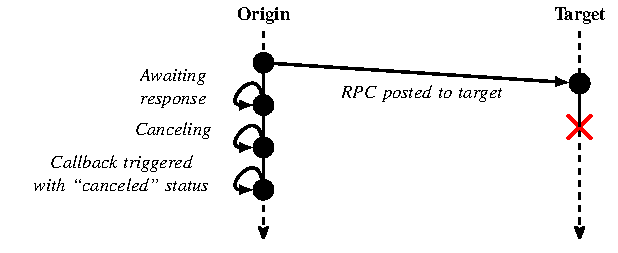
\includegraphics{figs/cancel}
%\vspace{-5pt}
\caption{Cancelation of an RPC operation.}
\label{fig:cancel}
%\vspace{-5pt}
\end{figure}

Cancelation of operations in Mercury is always an \textit{asynchronous} and
\textit{local} operation. As shown in Figure~\ref{fig:cancel}, forwarding an RPC
request is a nonblocking operation. Therefore, since Mercury follows a callback-based
mechanism, completion of that operation is known from a user's
perspective only when the callback that is associated to that operation
is pushed to the local completion queue and later triggered after making both
progress and trigger calls. When that callback is triggered, the state of the
operation is reported to the user as \textit{canceled}. Since operations are nonblocking,
keeping cancelation an asynchronous operation instead of an operation that completes
immediately is essential.
This mechanism protects against races in the event that a peer response arrives
after local cancelation has already succeeded. After the callback is triggered,
it is then safe to re-use the existing RPC request handle to issue a retry for example.

Cancelation is the foundation for implementing timeout scenarios in data services
in order to recover from a fault. When an internal
fault occurs, however, cancelation of the operation is not always necessary if the RPC
has not yet been posted, in which case that operation can simply be directly retried. This
scenario is similar for all other nonblocking operations in Mercury, including
bulk data transfers.

\section{Applications and Use Cases}
\label{sec:apps}

As mentioned in Section~\ref{sec:intro}, Mercury is part of the Mochi suite of service of components.
Mochi provides additional features on top of Mercury such as the notion of group membership,
transparent user-level thread semantics, key/value stores, C++ and Python bindings.
This work is further described in~\cite{Ross2020} along with
additional use cases, including the following:

Intel's \textit{Distributed Application Object Storage} (DAOS)~\cite{Intel2019} project
provides a transactional and multidimensional object store for
use in large-scale HPC environments with embedded storage directly
attached to the compute fabric. DAOS is a vendor-backed push to
provide an alternative to the traditional parallel file system and has the
potential to extract higher performance out of emerging low latency storage
technology by running in user space. DAOS is envisioned as a multiuser and persistent
volume available to all applications. It therefore encompasses a variety of
system management capabilities, including distributed authentication and
device provisioning.

The \textit{Unify} project, the successor to BurstFS~\cite{Wang2016},
implements a temporary high-performance file system using
local resources on nodes in the HPC system. In Unify, data is
explicitly staged between the temporary Unify file system and the
``permanent'' parallel file system. The Unify team is exploring
specialization in the form of multiple flavors of file systems, such
as \textit{UnifyCR} for
checkpoint/restart workloads and a
separate specialized version for machine learning workloads. This backend
specialization allows Unify to optimize for different use cases without
sacrificing the portability and common toolset advantages of a POSIX
interface. UnifyCR, for example, uses user-space I/O interception,
scalable metadata indexing, and colocated I/O delegation to optimize
bursty checkpoint workloads while still presenting a traditional file
system view of the data.

\textit{GekkoFS}~\cite{Vef2018} implements a temporary and
highly scalable file system providing relaxed POSIX semantics tailored
to the majority of HPC applications. This type of specialization
allows applications using the existing POSIX interface (under
specific constraints) to see dramatic performance improvements
as compared with file systems supporting the complete specification. The
GekkoFS team has demonstrated millions of metadata operations per
second, allowing it to serve applications with access patterns that
were historically poor matches for file systems, and the team has shown rapid
service instantiation times allowing new GekkoFS volumes to be started
on a per-job basis.

\textit{Proactive Data Containers} (PDC)~\cite{Mu2018} provides a data
model in which a container holds a collection of objects that may
reside at different levels of a potentially complex storage hierarchy and
migrate between them. A PDC volume is instantiated for an application
workflow and sized to meet workflow requirements for data storage
and I/O. Objects can hold both streams of bytes and KV pairs,
and additional metadata can be associated with objects as well.
Unlike GekkoFS and UnifyCR, PDC does not present a conventional file
system interface but instead provides a way of unifying application's memory
and storage by providing object mapping semantics, which hide actual I/O transfers
between storage hierarchies from the user.

\section{Conclusion}
\label{sec:concl}

To support data services at scale, a re-usable RPC component must be able
to provide performance by enabling the use of all the underlying hardware and
network fabrics, flexibility by facilitating service composition, and resilience
by providing support for local cancelation. Mercury in that regard is
already providing this functionality and is on the path of being used on
production systems, to enable not only file system capabilities but to also
provide specialized data service workflows as part of the Mochi suite of
components.

We are also considering how to make use of
collectives through Mercury and how to provide data services with
optimized collective RPC operations (such as RPC broadcasts) that do not only
rely on point-to-point messaging, which is a limitation when an RPC
must be sent to a large number of targets.
Furthermore, with accelerators (e.g., GPUs) that are now part of the HPC ecosystem, there
is a growing interest in how to make efficient use of RDMA and address the accelerator's 
memory directly from a remote target. These are two future directions
that we are considering to further evolve our RPC framework.

\section*{Acknowledgments}

This material was based upon work supported in part by the U.S. Department
of Energy, Office of Science, Advanced Scientific Computing Research
program, under Contract No. DE-AC02-06CH11357; in part supported by
the Exascale Computing Project (17-SC-20-SC), a joint project of the
U.S. Department of Energy`s Office of Science and National Nuclear
Security Administration.  responsible for delivering a capable exascale
ecosystem, including software, applications, and hardware technology,
to support the nation`s exascale computing imperative; and in part
supported by the U.S. Department of Energy, Office of Science, Office
of Advanced Scientific Computing Research, Scientific Discovery through
Advanced Computing (SciDAC) program.

This research used resources of the Argonne Leadership Computing
Facility, which is a DOE Office of Science User Facility supported
under Contract DE-AC02-06CH11357.

The authors would like to thank Howard Pritchard for his help on
successfully porting this software to Cray GNI-based systems.

\begin{thebibliography}{10}
\itemsep=1pt
\begin{small}

\bibitem{mpich}
{Argonne National Laboratory}, ``{MPICH},'' 2013. [Online]. Available:
  \url{http://www.mpich.org}

\bibitem{Zounmevo2013}
J.~Zounmevo, D.~Kimpe, R.~Ross, and A.~Afsahi, ``{On the Use of MPI in
  High-Performance Computing Services},'' in \emph{Recent Advances in the
  Message Passing Interface}, 2013.

\bibitem{protobuf}
{Google Inc}, ``{Protocol Buffers},'' 2012. [Online]. Available:
  \url{https://developers.google.com/protocol-buffers}

\bibitem{Slee2007}
M.~Slee, A.~Agarwal, and M.~Kwiatkowski, ``{Thrift: Scalable Cross-Language
  Services Implementation},'' Facebook, 156 University Ave, Palo Alto, CA,
  Tech. Rep., 2007.

\bibitem{Wang2009}
F.~Wang, S.~Oral, G.~Shipman, O.~Drokin, T.~Wang, and I.~Huang,
  ``{Understanding Lustre Filesystem Internals},'' Oak Ridge National Lab.,
  National Center for Computational Sciences, Tech. Rep., 2009,
  {O}RNL/TM-2009/117.

\bibitem{Welch2008}
B.~Welch, M.~Unangst, Z.~Abbasi, G.~Gibson, B.~Mueller, J.~Small, J.~Zelenka,
  and B.~Zhou, ``{Scalable Performance of the Panasas Parallel File System},''
  in \emph{Proceedings of the 6th USENIX Conference on File and Storage
  Technologies}, ser. FAST’08.\hskip 1em plus 0.5em minus 0.4em\relax USA:
  USENIX Association, 2008.

\bibitem{Ali2009}
N.~Ali, P.~Carns, K.~Iskra, D.~Kimpe, S.~Lang, R.~Latham, R.~Ross, L.~Ward, and
  P.~Sadayappan, ``{Scalable I/O Forwarding Framework for High-Performance
  Computing Systems},'' in \emph{IEEE International Conference on Cluster
  Computing and Workshops}, 2009, pp. 1--10.

\bibitem{Sandberg1988}
R.~Sandberg, D.~Golgberg, S.~Kleiman, D.~Walsh, and B.~Lyon, \emph{Design and
  Implementation of the Sun Network Filesystem}.\hskip 1em plus 0.5em minus
  0.4em\relax USA: Artech House, Inc., 1988, pp. 379--390.

\bibitem{Soumagne2013}
J.~{Soumagne}, D.~{Kimpe}, J.~{Zounmevo}, M.~{Chaarawi}, Q.~{Koziol},
  A.~{Afsahi}, and R.~{Ross}, ``{Mercury: Enabling Remote Procedure Call for
  High-Performance Computing},'' in \emph{2013 IEEE International Conference on
  Cluster Computing (CLUSTER)}, Sep. 2013, pp. 1--8.

\bibitem{Ross2020}
R.~B. Ross, G.~Amvrosiadis, P.~Carns, C.~D. Cranor, M.~Dorier, K.~Harms,
  G.~Ganger, G.~Gibson, S.~K. Gutierrez, R.~Latham, B.~Robey, D.~Robinson,
  B.~Settlemyer, G.~Shipman, S.~Snyder, J.~Soumagne, and Q.~Zheng, ``{Mochi:
  Composing Data Services for High-Performance Computing Environments},''
  \emph{Journal of Computer Science and Technology}, vol.~35, no.~1, pp.
  121--144, Jan 2020. [Online]. Available:
  \url{https://doi.org/10.1007/s11390-020-9802-0}

\bibitem{Docan2012}
C.~Docan, M.~Parashar, and S.~Klasky, ``{DataSpaces: An Interaction and
  Coordination Framework for Coupled Simulation Workflows},'' \emph{Cluster
  Computing}, vol.~15, no.~2, pp. 163--181, Jun. 2012. [Online]. Available:
  \url{https://doi.org/10.1007/s10586-011-0162-y}

\bibitem{Docan2010}
------, ``{Enabling High-speed Asynchronous Data Extraction and Transfer Using
  DART},'' \emph{Concurr. Comput. : Pract. Exper.}, vol.~22, no.~9, pp.
  1181--1204, 2010.

\bibitem{Wood2016}
C.~Wood, S.~Sane, D.~Ellsworth, A.~Gimenez, K.~Huck, T.~Gamblin, and A.~Malony,
  ``"a scalable observation system for introspection and in situ analytics",''
  in \emph{Proceedings of the 5th Workshop on Extreme-Scale Programming Tools},
  ser. ESPT ’16.\hskip 1em plus 0.5em minus 0.4em\relax IEEE Press, 2016, pp.
  42--49.

\bibitem{Ulmer2018}
C.~Ulmer, S.~Mukherjee, G.~Templet, S.~Levy, J.~Lofstead, P.~Widener,
  T.~Kordenbrock, and M.~Lawson, ``"faodel: Data management for next-generation
  application workflows",'' in \emph{Proceedings of the 9th Workshop on
  Scientific Cloud Computing}, ser. ScienceCloud’18.\hskip 1em plus 0.5em
  minus 0.4em\relax New York, NY, USA: Association for Computing Machinery,
  2018. [Online]. Available: \url{https://doi.org/10.1145/3217880.3217888}

\bibitem{Lofstead2011}
J.~Lofstead, R.~Oldfield, T.~Kordenbrock, and C.~Reiss, ``{Extending
  Scalability of Collective IO through Nessie and Staging},'' in
  \emph{Proceedings of the Sixth Workshop on Parallel Data Storage}.\hskip 1em
  plus 0.5em minus 0.4em\relax New York, NY, USA: ACM, 2011, pp. 7--12.

\bibitem{Grun2015}
P.~{Grun}, S.~{Hefty}, S.~{Sur}, D.~{Goodell}, R.~D. {Russell}, H.~{Pritchard},
  and J.~M. {Squyres}, ``{A Brief Introduction to the OpenFabrics Interfaces -
  A New Network API for Maximizing High Performance Application Efficiency},''
  in \emph{2015 IEEE 23rd Annual Symposium on High-Performance Interconnects},
  Aug 2015, pp. 34--39.

\bibitem{Intel2019}
{Intel Corporation}, ``{DAOS: Revolutionizing High-Performance Storage with
  Intel Optane Technology},''
  \url{https://www.intel.com/content/dam/www/public/us/en/documents/solution-briefs/high-performance-storage-brief.pdf},
  Jun. 2019.

\bibitem{Wang2016}
T.~{Wang}, K.~{Mohror}, A.~{Moody}, K.~{Sato}, and W.~{Yu}, ``{An Ephemeral
  Burst-Buffer File System for Scientific Applications},'' in \emph{SC '16:
  Proceedings of the International Conference for High Performance Computing,
  Networking, Storage and Analysis}, Nov 2016, pp. 807--818.

\bibitem{Vef2018}
M.~{Vef}, N.~{Moti}, T.~{Süß}, T.~{Tocci}, R.~{Nou}, A.~{Miranda},
  T.~{Cortes}, and A.~{Brinkmann}, ``{GekkoFS---A Temporary Distributed File
  System for HPC Applications},'' in \emph{2018 IEEE International Conference
  on Cluster Computing (CLUSTER)}, Sep. 2018, pp. 319--324.

\bibitem{Mu2018}
J.~{Mu}, J.~{Soumagne}, H.~{Tang}, S.~{Byna}, Q.~{Koziol}, and R.~{Warren},
  ``{A Transparent Server-Managed Object Storage System for HPC},'' in
  \emph{2018 IEEE International Conference on Cluster Computing (CLUSTER)},
  Sep. 2018, pp. 477--481.

\end{small}
\end{thebibliography}

\end{document}

\end{article}

\makeatletter
\renewcommand{\AB@affillist}{}
\renewcommand{\AB@authlist}{}
\setcounter{authors}{0}
\makeatother

\begin{article}
{Extending the Publish/Subscribe Abstraction for High-Performance I/O and Data Management at Extreme Scale}
{Jeremy Logan, Mark Ainsworth, Chuck Atkins, Jieyang Chen, Jong Choi, Junmin Gu, James Kress, Greg Eisenhauer, Berk Geveci, William Godoy, Mark Kim, Tahsin Kurc, Qing Liu, Kshitij Mehta, George Ostrouchov, Norbert Podhorzski, David Pugmire, Eric Suchyta, Nicolas Thompson, Ozan Tugluk, Lipeng Wan, Ruonan Wang, Ben Whitney, Matthew Wolf, Kesheng Wu and Scott Klasky}
\graphicspath{{submissions/jeremy/}}
%\documentclass[11pt,dvipdfm]{article}
\documentclass[11pt]{article}
\usepackage{deauthor,times,graphicx} %required
\usepackage{amsmath,amssymb}
\usepackage{multirow}
\usepackage{algorithm}
\usepackage{algpseudocode}
\usepackage{todonotes}
\usepackage{url}

% \graphicspath{{farnadi/}}

\newtheorem{mydef}{\textbf{Definition}}
\newtheorem{myex}{\textbf{Example}}
\newtheorem{mytheorem}{\textbf{Theorem}}


\begin{document}

\title{A Declarative Approach to Fairness in Relational Domains}
\author{Golnoosh Farnadi$^{1,2}$, Behrouz Babaki$^1$, Lise Getoor$^3$\\
$^1$Polytechnique Montr\'{e}al, $^2$ Mila, $^3$ UC Santa Cruz \\
farnadig@mila.quebec, behrouz.babaki@polymtl.ca, getoor@soe.ucsc.edu}

\maketitle

\begin{abstract}
AI and machine learning tools are being used with increasing frequency for decision making in domains that affect peoples' lives such as employment, education, policing and %loan approval
financial qualifications. These uses raise concerns about biases of algorithmic discrimination and have motivated the development of fairness-aware machine learning. However, existing fairness approaches are based solely on attributes of individuals. In many cases, discrimination is much more complex, and taking into account the social, organizational, and other connections between individuals is important. We introduce new notions of fairness that are able to capture the relational structure in a domain. We use first-order logic to provide a flexible and expressive language for specifying complex relational patterns of discrimination. Furthermore, we extend an existing statistical relational learning framework, probabilistic soft logic~(PSL), to incorporate our definition of relational fairness. We refer to this fairness-aware framework FairPSL. FairPSL makes use of the logical definitions of fairnesss but also supports a probabilistic interpretation. In particular, we show how to perform maximum a posteriori~(MAP) inference by exploiting probabilistic dependencies within the domain while avoiding violations of fairness guarantees. Preliminary empirical evaluation shows that we are able to make both accurate and fair decisions.
\end{abstract}

\section{Introduction}
\label{sec:introduction}

Over the past few years, AI and machine learning have become essential components in operations that drive the modern society, e.g., in financial, administrative, and educational spheres. \emph{Discrimination} happens when qualities of individuals which are not relevant to the decision making process influence the decision. Delegating decision making to an automated process raises questions about discriminating against individuals with certain traits based on biases in the data. This is especially important when the decisions have the potential to impact the lives of individuals, for example, the decisions on granting loans, assigning credit, and employment. 

\emph{Fairness} is defined as the absence of discrimination in a decision making process. The goal of \emph{fairness-aware} machine learning is to ensure that the decisions made by an algorithm do not discriminate against a population of individuals~\cite{feldman2015certifying2,boyd2014networked,hardt2016equality3}. Fairness has been well studied in the social sciences and legal scholarship (for an in-depth review see~\cite{barocas2016big2}), and there is emerging work on fairness-aware ML within the AI and computer science communities. For example, fairness through awareness/Lipschitz property~\cite{dwork2012fairness3}, individual fairness~\cite{zemel2013learning}, statistical parity/group fairness~\cite{kamishima2011fairness}, counterfactual fairness~\cite{counterfactualfairness}, demographic parity/disparate impact~\cite{feldman2015certifying2,chouldechova2017fair2}, preference-based fairness~\cite{zafar2017parity}, and equality of opportunity~\cite{hardt2016equality3}.

The existing work in fairness-aware machine learning is based on a definition of discrimination where a decision is influenced by an \emph{attribute} of an individual. An attribute value upon which discrimination is based (such as gender, race, or religion) is called a \emph{sensitive attribute}. The sensitive attribute defines a population of vulnerable individuals known as the \emph{protected group}. A fair decision-making process treats the protected group the same as the \emph{unprotected group}. 

However, in many social contexts, discrimination is the result of complex interactions and can not be described solely in terms of attributes of an individual. For example, consider an imaginary scenario in an organization in which younger female workers who have older male supervisors have lower chances of promotion than their male counterparts.\footnote{Of course, many other patterns may be possible: female bosses may promote female subordinates and discriminate against male workers, or male bosses may promote female employees.  Our goal is to provide a general framework which is able to describe arbitrarily complex discrimination patterns.} 
 This discrimination pattern involves two attributes of the individual (gender and age), a relationship with another individual (supervisor), and two attributes of the second individual. Addressing such complex cases poses two challenges. First, the concepts of discrimination and fairness need to be extended to capture not only attributes of individuals but also the relationships between them. Second, a process is required that ensures that fair decisions are made about individuals who are affected by such patterns. In this paper we address both of these challenges.
We use first-order logic (FOL) to extend the notion of fairness to the relational setting. FOL is an expressive representation for relational problems which is also widely used for learning in relational domains. Moreover, we extend an existing framework for statistical relational learning~\cite{getoor2007introduction} called probabilistic soft logic (PSL)\footnote{http://psl.linqs.org/}~\cite{bach:jmlr17}. PSL combines logic and probability for learning and reasoning over uncertain relational domains. One of the most common reasoning tasks in PSL is called maximum a posteriori (MAP) inference, which is performed by finding the most probable truth values for unknowns over a set of given evidence. We develop a new MAP inference algorithm which is able to maximize the a posteriori values of unknown variables \emph{subject to} fairness guarantees. An early version of this paper which this work builds upon and extends appeared in~\cite{farnadi2018fairness}.

\looseness-1
Our contributions are as follows: 1) we propose fairness-aware machine learning for the relational setting; 2) we extend PSL into a fairness-aware framework called FairPSL which can represent the logical definition of fairness; 3) we develop a new MAP inference algorithm which is able to maximize the posteriori values of unknown variables \emph{subject to} fairness guarantees; 4) we empirically evaluate our proposed framework on synthetic data. 

\section{Motivation}
\label{sec:motivation}

Discrimination in social contexts have been studied in the field of social psychology~\cite{brewer2007social,brewer1979group,ridgeway2004unpacking}. There is a large literature on various aspects of relational bias in social contexts such as \emph{in-group-out-group bias}, \emph{gender bias}, and \emph{ethnicity-based favoritism} that can result in discrimination. 
As an example, consider gender bias in the workplace that reflects stereotypically masculine criteria and male-based favoritism. Such gender bias 
typically places women in lower positions and negatively impacts their opportunities. Further, lack of women in leadership positions may affect the promotion of women and results in a glass ceiling that keeps women from rising beyond a certain level in the hierarchy. This scenario shows that considering  protected attributes such as gender is not always sufficient to detect the source of bias and avoid discrimination, one also has to consider the relational information, in this case the organization hierarchy. Note that this can be generalized to any ingroup/outgroup scenario where the sensitive attribute could be race, religion, age, marital-status, etc.

The existing work on designing fair algorithms in machine learning exclusively focuses on \emph{attribute-based fairness}, which is based on the following assumptions: First, there is an assumption that the individuals (sometimes referred to as units or entities) are independent and described by simple attribute vectors. Second, the group for which one wishes to ensure fairness (known as the \emph{protected group}) is defined on the basis of some attribute values. Finally, there is a decision that is associated with each individual, and the goal is to ensure that members of the protected group are subject to a fair decision (we discuss different fairness measures in Section~\ref{sec:fairnessmeasure}).  We illustrate  attribute-based fairness in the following example. 

\begin{myex}[Loan Processing]
\label{ex:loan}
A bank bases its decisions about granting a loan on attributes of the applicant. The goal is to decide whether to grant a loan to an applicant using a predictive model. The bank needs to ensure that the obey fair lending practices and ensure that gender, race, sexual orientation of applicants has no influence on the decision. In this scenario, the protected group is the historically disadvantaged applicants.  
\end{myex}
The current fairness-aware machine learning techniques are not capable of modeling relations and hence cannot be used to make the decision making model fair. However, in many decision making scenarios, especially in social and organizational settings, the domain is relational, and the protected group itself might be best represented using a relational definition. We illustrate this setting in the following scenario:
\begin{myex}[Performance Review]
\label{ex:review}
Consider an organization where decisions about the promotion of employees is based on two criteria: 1) an objective performance measure, and 2) the opinion of their direct and indirect managers above them. The opinions are inferred from the performance reviews which are collected periodically. Not every manager can submit a review for all its subordinates, this is especially the case for top-level managers who have a large number of subordinates. Hence, the opinions of managers are collectively inferred from the opinions of their sub-ordinates. However, some employees may be biased, and judge other employees unfavorably, by favoring employees who are similar to themselves (same gender, race, religion, etc.) over employees who are dissimilar. The organization needs to ensure that promotion of employees do not have any relational bias caused by in-group-out-group favoritism.

\end{myex}
Example~\ref{ex:review} describes a prediction problem over a database that consists of relations between employees. Such prediction tasks are best handled by techniques from the relational learning domain. To ensure fair prediction in such settings, we need to extend the notion of \emph{attribute-based fairness} to \emph{relational fairness}. Throughout this paper, we use the performance review problem as a running example for relational fairness.

\section{Fairness Formalism}
\label{sec:formulation}

A representation that can describe different types of entities and different relationships between them is called relational. In this section, we use first-order logic to define relational fairness. We employ first-order logic as an expressive representation formalism which can represent objects and complex relationships between them. We start by defining an atom:

\begin{mydef}[Atom]
An atom is an expression of the form $P(a_1, a_2, \ldots, a_n)$ where each argument $a_1, a_2,$ $\ldots,$ $a_n$ is either a constant or a variable. The finite set of all possible substitutions of a variable to a constant for a particular variable $a$ is called its \textit{domain} $D_{a}$. If all variables in $P(a_1, a_2, \ldots, a_n)$ are substituted by some constant from their respective domain, then we call the resulting atom a \textit{ground atom}. 
\end{mydef}

\begin{myex}
In our loan processing problem (Example~\ref{ex:loan}), we can represent applicants' attributes by atoms. For instance, atom $Female(v)$ indicates whether or not applicant $v$ is female. Similarly, we can represent relations with atoms. In the performance review problem in Example~\ref{ex:review} the atom $Manager(m,e)$ indicates whether or not employee $m$ is a direct or indirect manager of employee $e$.
\end{myex}

The relational setting provides the flexibility to express complex definitions with formulae.

\begin{mydef}[Formula] 
A formula is defined by induction: every atom is a formula. If $\alpha$ and $\beta$ are formulae, then $\alpha \vee \beta$, $\alpha \wedge \beta$, $\neg \alpha$, $\alpha \rightarrow \beta$ are formulae. If $x$ is a variable and $\alpha$ is a formula, then the quantified expressions of the form $\exists x$ $\alpha$ and $\forall x$ $\alpha$ are formulae.    
\end{mydef}

To characterize groups of individuals based on a formula, we define the notion of \emph{population}.

\begin{mydef}[Population]
We denote formula $F$ which has only one free variable $v$ (i.e., other variables in $F$ are quantified) by $F[v]$. The population defined by $F[v]$ is the set of substitutions of $v$ for which $F[v]$ holds.   
\end{mydef}


\begin{myex}
\label{ex:disformula}
Consider the formula $F[v] := \forall u, \, \textit{Manager}(u,v) \rightarrow \neg \textit{SameGroup}(u, v)$. The population specified by this formula is the set of individuals all of whose managers belong to a group different from theirs. 
\end{myex}

The truth value of a formula is derived from the truth value of atoms that it comprises, according to the rules of logic. Each possible assignment of truth values to ground atoms is called an \emph{interpretation}. 


\begin{mydef}[Interpretation]
An interpretation $I$ is a mapping that associates a truth value $I(P)$ to each ground atom $P$. For Boolean truth values, $I$ associates true to 1 and false to 0 truth values. For soft logic (see Definition~\ref{def:softlogic}) $I$ maps each ground atom $P$ to a truth value in interval $[0, 1]$.
\end{mydef}

In attribute-based fairness, it is assumed that there is a certain attribute of individuals, i.e, the sensitive attribute,  that we do not want to affect a decision. Gender, race, religion and marital status are examples of sensitive attributes. Discrimination has been defined in social science studies as a treatment in favor or against a group of individuals given their sensitive attribute. This group of individuals is the protected group. 

In a relational setting, both the sensitive attributes of an individual and their participation in various relations may have an undesired effect on the final decision. We characterize the protected group in a relational setting by means of a population. In practice, we are often interested in maintaining fairness for a specific population such as applicants, students, employees, etc. This population is then partitioned into the protected and unprotected groups. We define a \emph{discriminative pattern} which is a pair of formulae to capture these groups: 1) $F_1[v]$: to specify the difference between the protected and unprotected groups and 2) $F_2[v]$: to specify the population over which we want to maintain fairness. 

\begin{mydef}[Discriminative pattern]
A discriminative pattern is a pair $\textit{DP}[v]:=(F_1[v], F_2[v])$ , where $F_1[v]$ and $F_2[v]$ are formulae.
\end{mydef}

\begin{myex}
\label{ex:pattern}
The two formulae in the discrimination pattern $\textit{DP}[v]:= \big((\forall u, \,  \textit{Manager}(u,v) \rightarrow  \neg \textit{SameGroup}(u, v)),$ $\textit{Employee}(v)\big)$ specify two populations, namely all employees and those employees who belong to a group different from their managers.
\end{myex}

Given the definition of the discriminative pattern, we have a rich language to define the scope of the protected and unprotected groups in a relational setting.

\begin{mydef}[Protected group] Given an interpretation $I$, the protected group is a population of the form:
{$$PG :=\{ v : F_1[v] \wedge F_2[v]\}$$}
which is defined as the set of all instances hold for variable $v$ for which $F_1[v] \wedge F_2[v]$ is true under interpretation $I$, that is, $I(F_1[v] \wedge F_2[v]) = 1$. 
Similarly, the \emph{unprotected group} is a population of the form: 
{$$UG := \{ v : \neg F_1[v] \wedge  F_2[v]\}$$}
which is defined as the set of all instances hold for variable $v$ 
for which $I(\neg F_1[v] \wedge F_2[v]) = 1$. 
\end{mydef}

\begin{myex}
The protected group of the discrimination pattern specified in Example~\ref{ex:pattern} is {$PG := \big\{ v : \big(\forall u, \,$ $ \textit{Manager}(u, v) \rightarrow \neg \textit{SameGroup}(u, v)\big) \wedge \textit{Employee}(v) \big\}$} and the unprotected group is {$UG :=  \big\{ v:  \big(\exists u, \, \textit{Manager}(u,v) \wedge \textit{SameGroup}(u, v)\big) \wedge \textit{Employee}(v) \big\}$}. This means our protected group is the set of employees belonging to a group different from their managers,
and our unprotected group consists of other employees. 
\end{myex}

Discrimination is defined in terms of a treatment or decision that distinguishes between the protected and unprotected groups. Here we define the \emph{decision} atom.
\begin{mydef}[Decision atom] A decision atom $d(v)$ is an atom containing exactly one variable $v$ that specifies a decision affecting the protected group which is defined either by law or end-user.
\end{mydef}
\begin{myex}
The decision atom ${\textit ToPromote}(v)$ indicates whether or not $v$ receives a promotion.
\end{myex}

Note that the fairness formulation in this section is designed for the relational setting, however relational fairness subsumes the attribute-based fairness such that: a sensitive attribute is defined by an atom with one argument and $F_2[v]$ in discrimination pattern is $\textit{Applicant}(v)$. For example, discrimination pattern of our loan processing problem in Example~\ref{ex:loan} is of the form $\textit{DP} := ( \textit{Female}(v), \textit{Applicant}(v))$ that denotes female applicants as the protected group (i.e., $PG :=  \{ v: \textit{Female}(v) \}$) and male applicants as the unprotected group (i.e., $UG := \{ v: \neg \textit{Female}(v)\}$).


\section{Fairness Measures}
\label{sec:fairnessmeasure}

Over the past few years, many fairness measures have been introduced~\cite{verma2018fairness2}. An important class of these measures are \emph{group fairness} measures which quantify the inequality between different subgroups. Some of the most popular measures in this class include \emph{equal opportunity}, \emph{equalized odds}, and \emph{demographic parity}~\cite{hardt2016equality3}. In this paper we restrict our focus to the latter. In an attribute-value setting, demographic parity means that the decision should be independent of the protected attributes. Assume that binary variables $A$ and $C$ denote the decision and protected attributes, and the preferred value of $A$ is one. Demographic parity requires that:

\begin{equation*}
    P(A=1 | C=0) = P(A=1 | C=1)
\end{equation*}

We will now generalize this measure to the relational setting using the notations defined in Section~\ref{sec:formulation}. Let $a$ and $c$ denote the counts of denial (i.e., negative decisions) for protected and unprotected groups, and $n_{1}$ and $n_{2}$ denote their sizes, respectively. Given the decision atom $d(v)$, discriminative pattern $\textit{DP}(F_1[v], F_2[v])$, and interpretation $I$, these counts are computed by the following equations: 
{
\begin{flalign}
    & a \equiv \sum_{v \in D_v} I\big( \neg d(v) \wedge  F_1[v] \wedge F_2[v]) \label{eq:a}\\
    & c \equiv \sum_{v \in D_v} I\big( \neg d(v) \wedge  \neg F_1[v] \wedge  F_2[v]) \label{eq:c}\\
    & n_{1} \equiv \sum_{v \in D_v} I\big(F_1[v] \wedge F_2[v]) \label{eq:n1}\\
    & n_{2} \equiv \sum_{v \in D_v} I\big(\neg F_1[v] \wedge  F_2[v]) \label{eq:n2}
\end{flalign}}
The proportions of denying for protected and unprotected groups are $p_1 = \frac{a}{n_1}$ and $p_2 = \frac{c}{n_2}$, respectively. There are a number of data-driven measures~\cite{Pedreschi:2012} which quantify demographic disparity and can be defined in terms of $p_1$ and $p_2$:
\begin{itemize}
    \item \textbf{Risk difference}: $RD = p_1 - p_2$, also known as absolute risk reduction. 
    \item \textbf{Risk Ratio}: $RR = \frac{p_1}{p_2}$, also known as relative risk. 
    \item \textbf{Relative Chance}: $RC = \frac{1 - p_1}{1 - p_2}$ also, known as selection rate.
\end{itemize}
These measures have been used in the legal systems of European Union, UK, and US~\cite{EUlaw,UKlaw,USlaw}. Notice that RR is the ratio of the proportion of benefit denial between the protected and unprotected groups, while RC is the ratio of the proportion of benefit granted. Finally, we introduce the notion of $\delta$-fairness.

\begin{mydef}[$\delta$-fairness]
If a fairness measure for a decision making process falls within some $\delta$-window, then the process is \emph{$\delta\text{-fair}$}. Given $0 \leq \delta \leq 1$, the  $\delta$-windows for measures RD/RR/RC are defined as:
{\begin{flalign*}
	     - \delta \leq &RD \leq \delta \\
	     1- \delta \leq &RR \leq 1+ \delta\\
	     1- \delta \leq &RC \leq 1+ \delta
	\end{flalign*}}
\end{mydef}

To overcome the limitations of attribute-based fairness, we introduce a new statistical relational learning~(SRL) framework~\cite{getoor2007introduction} suitable for modelling fairness in relational domain. In the next section, we review probabilistic soft logic~(PSL). We then extend PSL with the definition of relational fairness introduced above in Section~\ref{sec:fairMAP}. Our fairness-aware framework, ``FairPSL'', is the first SRL framework that performs fair inference. 

\section{Background: Probabilistic Soft Logic}
\label{sec:psl}

In this section, we review the syntax and semantics of PSL, and in the next section we extend MAP inference in PSL with fairness constraints to define MAP inference in FairPSL.

PSL is a probabilistic programming language for defining hinge-loss Markov random fields~\cite{bach:jmlr17}. Unlike other SRL frameworks whose atoms are Boolean, atoms in PSL can take continuous values in the interval $[0,1]$. PSL is an expressive modeling language that can incorporate domain knowledge with first-order logical rules and has been used successfully in various domains, including bioinformatics~\cite{sridhar:bioinformatics16}, recommender systems~\cite{kouki:recsys15}, natural language processing~\cite{ebrahimi:emnlp16}, information retrieval~\cite{alshukaili:iswc16}, and social network analysis~\cite{west2014exploiting}, among many others. 
 
A PSL model is defined by a set of first-order logical rules called \emph{PSL rules}.

\begin{mydef} [PSL rule] a PSL rule $r$ is an expression of the form:
{\begin{equation}
\lambda_{r}: T_1 \land T_2 \land \ldots \land T_w \rightarrow H_1 \vee H_2 \vee \ldots \vee H_l
\end{equation}}

where { $T_1, T_2, \ldots, T_w, H_1, H_2, \ldots, H_l$} are atoms or negated atoms and { $\lambda_{r} \in \mathbb{R}^{+} \cup \infty$} is the weight of the rule $r$.  We call { $T_1 \land T_2 \land \ldots \land T_w$} the body of $r$ ($r_{body}$), and { $H_1 \vee H_2 \vee \ldots \vee H_l$} the head of $r$ ($r_{head}$).
\end{mydef}


Since atoms in PSL take on continuous values in the unit interval $[0,1]$, next we define soft logic to calculate the value of the PSL rules under an interpretation $I$.

\begin{mydef}[Soft logic]
\label{def:softlogic}
The ({$\tilde{\wedge}$}) and ({$\tilde{\vee}$}) and negation ({$\tilde{\neg}$}) are defined as follows. For {$m, n \in [0,1]$} we have: {$m \tilde{\wedge} n = \max(m+n -1, 0)$}, {$m \tilde{\vee} n = \min(m+n , 1)$} and {$\tilde{\neg} m = 1 - m$}. The $\, \tilde{} \,$ indicates the relaxation over Boolean values.
\end{mydef}

The probability of truth value assignments in PSL is determined by the rules' \emph{distance to satisfaction}.

\begin{mydef}[The distance to satisfaction]
The distance to satisfaction $d_{r}(I)$ of a rule $r$ under an interpretation $I$ is defined as:
{
\begin{equation}
d_{r}(I) = \max\{0, I(r_{body})-I(r_{head})\}
\end{equation}}
\end{mydef}

By using Definition~\ref{def:softlogic}, one can show that the closer the interpretation of a grounded rule $r$ is to 1, the smaller its distance to satisfaction. A PSL model induces a distribution over interpretations $I$. Let $R$ be the set of all grounded rules, then the probability density function is:
{
\begin{equation}
f(I) ={\frac{1}{Z}} \exp[-\sum_{r\in R} \lambda_{r}(d_{r}(I))^p]
\label{eq:potential}
\end{equation}
}
\noindent where { $\lambda_{r}$} is the weight of rule $r$, {
$Z = \int_{I} \exp[ -\sum_{r\in R} \lambda_{r}(d_{r}(I))^p]$
} is a normalization constant, and { $p \in \{1,2\}$} provides a choice of two different loss functions, $p=1$ (i.e., linear), and $p=2$ (i.e, quadratic). These probabilistic models are instances of hinge-loss Markov random fields~(HL-MRF)~\cite{bach:jmlr17}. The goal of maximum a posteriori (MAP) inference is to find the most probable truth assignments $I_{\textit{MPE}}$ of unknown ground atoms given the evidence which is defined by the interpretation $I$. Let $X$ be all the evidence, i.e., $X$ is the set of ground atoms such that $\forall x \in X, I(x)$ is known, and let $Y$ be the set of ground atoms such that $\forall y \in Y, I(y)$ is unknown. Then we have
{
\begin{equation}
I_{\textit{MAP}}(Y) = \textit{arg}\max_{I(Y)} P(I(Y)|I(X))
\end{equation}}
Maximizing the density function in Equation~\ref{eq:potential} is equivalent to minimizing the weighted sum of the distances to satisfaction of all rules in PSL. 

\begin{table*}[t]
    \centering
    \begin{tabular}{|lll|}
    \hline
    &&\\
    $R1$ & $\lambda_1$ &: $\textit{IsQualified}(e) \rightarrow \textit{HighPerformance}(e)$ \\
    $R2$ & $\lambda_1$ &: $\neg \textit{IsQualified}(e) \rightarrow \neg \textit{HighPerformance}(e)$ \\
    $R3$ & $\infty$ &: $\textit{PositiveReview}(e1, e2) \rightarrow \textit{PositiveOpinion}(e1, e2)$ \\
    $R4$ & $\infty$ &: $\neg \textit{PositiveReview}(e1, e2) \rightarrow \neg \textit{PositiveOpinion}(e1, e2)$ \\
    $R5$ & $\lambda_1$ &: $\textit{PositiveOpinion}(e1, e2) \wedge \textit{Manager}(m, e1) \rightarrow \textit{PositiveOpinion}(m, e2)$ \\
    $R6$ & $\lambda_1$ &: $\neg \textit{PositiveOpinion}(e1, e2) \wedge \textit{Manager}(m, e1) \rightarrow \neg \textit{PositiveOpinion}(m, e2)$ \\
    $R7$ & $\lambda_1$ &: $\textit{PositiveOpinion}(m, e) \wedge \textit{Manager}(m, e) \rightarrow \textit{IsQualified}(e)$ \\
    $R8$ & $\lambda_1$ &: $\neg \textit{PositiveOpinion}(m, e) \wedge \textit{Manager}(m, e) \rightarrow \neg \textit{IsQualified}(e)$ \\
    $R9$ &  $\lambda_1$ &: $\neg \textit{ToPromote}(e)$\\
    $R10$ & $\infty$ &: $\textit{IsQualified}(e) \rightarrow \textit{ToPromote}(e)$ \\
    $R11$ & $\infty$ &: $\neg \textit{IsQualified}(e) \rightarrow \neg \textit{ToPromote}(e)$ \\
    &&\\
    \hline
    \end{tabular}
    \caption{\small A simplified PSL model for the \emph{Performance Reviewing} problem}
    \label{tab:pslmodel}
\end{table*}

\begin{myex}
\label{ex:pslmodel}
The simplified PSL model for the performance reviewing problem in Example\ref{ex:review} is given in Table~\ref{tab:pslmodel}. The goal of MAP inference for this problem is to infer employees to promote. We simplified the model by assigning the same weight to all soft rules (i.e., $\lambda_i= 1$ where $i=\{1,2,5,6,7,8,9\}$). Below we explain the meaning of each rule in the model.

Rule $R1$ indicates that qualified employees have high performance and similarly rule $R2$ expresses that a negative qualification of employees is derived from their low performance. Rules $R5$ and $R6$ presents the propagation of opinion from bottom to top of the organizational hierarchy, i.e., managers have similar opinions towards employees given the opinions of their sub-ordinate managers. And rules $R7$ and $R8$ indicate that the positive/negative opinion of direct/indirect managers derive from the qualification of an employee. Rule $R9$ indicates the prior that not all employees get promoted. We also have four hard constraints (i.e., rules $R3$, $R4$, $R10$ and $R11$) where the weight of the rules are $\infty$. Rules $R3$ and $R4$ indicate that submitted positive/negative reviews should reflect positive/negative opinions. And two rules $R10$ and $R11$ show that a highly qualified employee should get promoted. 
\end{myex}

\section{Fairness-aware PSL (FairPSL)}
\label{sec:fairMAP}

The standard MAP inference in PSL aims at finding values that maximize the conditional probability of unknowns. Once a decision is made according to these values, one can use the fairness measure to quantify the degree of discrimination. A simple way to incorporate fairness in MAP inference is to add the $\delta$-fairness constraints to the corresponding optimization problem.   

Consider risk difference, $\textit{RD}$, where $\textit{RD} \equiv \frac{\mathbf{a}}{n_1} - \frac{\mathbf{c}}{n_2}$. The $\delta$-fairness constraint $-\delta \leq \textit{RD} \leq \delta$ can be encoded as the following constraints:
{\begin{align}
    & n_2 \mathbf{a} - n_1 \mathbf{c} - n_1 n_2 \delta \leq 0 \label{eq:RD1}\\
    & n_2 \mathbf{a} - n_1 \mathbf{c} + n_1 n_2 \delta \geq 0
\end{align}}
Similarly, from $\textit{RR} \equiv \frac{\mathbf{a} / n_1}{\mathbf{c} / n_2}$ and the $\delta$-fairness constraint $1 - \delta \leq \textit{RR} \leq 1 + \delta$ we obtain:
{\begin{align}
    & n_2 \mathbf{a} - (1 + \delta) n_1 \mathbf{c} \leq 0 \\
    & n_2 \mathbf{a} - (1 - \delta) n_1 \mathbf{c} \geq 0
\end{align}}
And finally, $\textit{RC} \equiv \frac{1 - \mathbf{a} / n_1}{1 - \mathbf{c} / n_2}$ and the $\delta$-fairness constraint $1 - \delta \leq \textit{RC} \leq 1 + \delta$ gives:
{ \begin{align}
    & - n_2 \mathbf{a} + (1 + \delta) n_1 \mathbf{c} - \delta n_1 n_2 \leq 0 \\
    & - n_2 \mathbf{a} + (1 - \delta) n_1 \mathbf{c} + \delta n_1 n_2 \geq 0 \label{eq:RC2}
\end{align}}
A primary advantage of PSL over similar frameworks is that its MAP inference task reduces to a convex optimization problem which can be solved in polynomial time. To preserve this advantage, we need to ensure that the problem will remain convex after the addition of $\delta$-fairness constraints. 

\begin{mytheorem}
The following condition is sufficient for preserving the convexity of MAP inference problem after addition of $\delta$-fairness constraints: The formulae $F_1[v]$ and $F_2[v]$ do not contain an atom $y \in Y$ and all atoms in $F_1[v]$ and $F_2[v]$ have values zero or one.
\end{mytheorem}
\begin{proof}
Since $I(F_1[v])$ and $I(F_2[v])$ do not depend on $I(Y)$, the values $n_{1}$ and $n_{2}$ are constants that can be computed in advance. Let us define the sets $D_v^a = \{ v \in D_v : F_1[v] \wedge F_2[v] \, \text{is true} \}$ and $D_v^c = \{ v \in D_v : \neg F_1[v] \wedge F_2[v] \, \text{is true} \}$. Since $F_1[v]$ and $F_2[v]$ can be only zero or one, we can rewrite the equations~\ref{eq:a} and \ref{eq:c} as:
{
\begin{align*}
    & \mathbf{a} = \sum_{v \in D_v^a} I(\neg d(v)) = |D_v^a| - \sum_{v \in D_v^a} I(d(v))\\
    & \mathbf{c} = \sum_{v \in D_v^c} I(\neg d(v)) = |D_v^c| - \sum_{v \in D_v^c} I(d(v))
\end{align*}}
\noindent which indicates that $\mathbf{a}$ and $\mathbf{c}$ can be expressed as linear combinations of variables in the optimization problem. This means that constraints~\ref{eq:RD1}-\ref{eq:RC2} are linear. Hence, addition of these constraints preserves the convexity of the optimization problem. 
\end{proof}

\section{Experiments}
\label{sec:experiment}

\begin{figure}
  \begin{minipage}[c]{0.6\textwidth}
    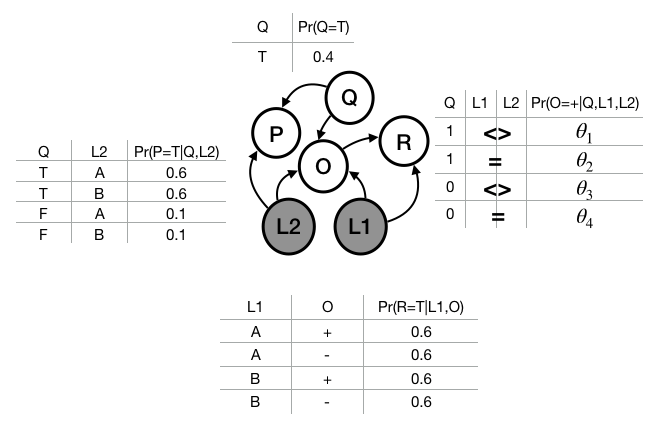
\includegraphics[width=\textwidth]{figs/BN.png}
  \end{minipage}\hfill
  \begin{minipage}[c]{0.45\textwidth}
    \caption{
        \small The model used for generating the datasets. There are four binary random variables, P, Q, O, and R. \textbf{P}: indicates whether or not the employee has high performance; \textbf{Q}: indicates whether or not an employee has high qualification; \textbf{O}: indicates whether or not the colleague submits the positive opinion towards the employee;  \textbf{R}: indicates whether or not the colleague has a positive opinion towards the employee;  \textbf{L1, L2}: indicates the label of the review provider and review receiver (observed).
    } \label{fig:BN}
  \end{minipage}
\end{figure}

We show the effectiveness of FairPSL by performing an empirical evaluation. We investigate two research questions in our experiments:
\begin{description}
\item[Q1] What is the effect of the fairness threshold $\delta$ on the fairness measures $RD/RC/RR$?
\item[Q2] How is decision quality affected by imposing $\delta$-fairness constraints?
\end{description}

Note that although we present the result for specific parameters of the framework in this section, we ran extensive analysis and the results we present are representative. We implemented the MAP inference routines of PSL and FairPSL in Python, using Gurobi-8.1\footnote{\url{www.gurobi.com}} as the backend solver. The FairPSL code, code for the data generator and data is publicly available\footnote{https://github.com/gfarnadi/FairPSL}. 

\subsection{Data generation}
  
We evaluate the FairPSL inference algorithm on synthetic datasets representing the performance review scenario (introduced in Example~\ref{ex:review}). The organization hierarchy is generated synthetically. 
The organization hierarchy generator is parameterized by two numbers: the number of employees in the organization ($n$) and the number of employees managed by each manager ($k$). Each employee is randomly assigned with a label \emph{A} or \emph{B}. An examples organization hierarchy with $n$=50 and $k$=3 is shown in Figure~\ref{fig:hierachy}.

\begin{figure}
  \begin{minipage}[c]{0.3\textwidth}
    \caption{
        \small An example of an organizational hierarchy with five levels and 50 employees with k=3. Each employee either has label A (shown with grey) or B (shown with white).
    }\label{fig:hierachy} 
	\end{minipage} \hfill
    \begin{minipage}[c]{0.7\textwidth}
    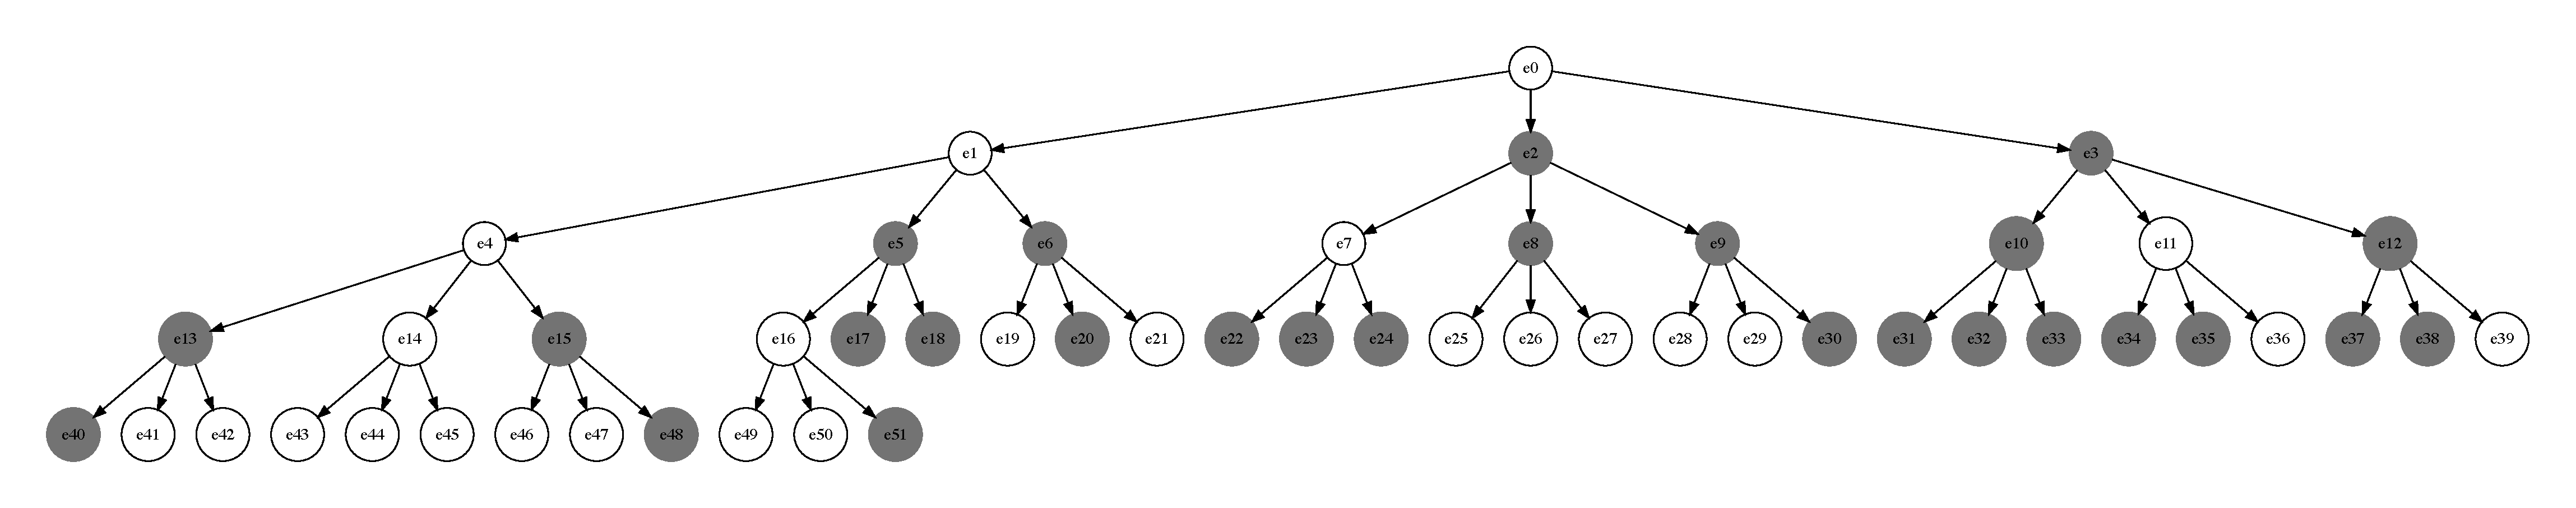
\includegraphics[width=\textwidth]{figs/Uni-hierachy.pdf}
  \end{minipage}
\end{figure}

For each employee, we use the generative model of Figure~\ref{fig:BN} to draw assignments for all the random variables. We assume that only $40\%$ of employees are qualified for promotion and regardless of their labels, employees submit only $60\%$ of their opinions. In addition, due to various personal and environmental factors, only $60\%$ of high quality employees perform well while $10\%$ of low quality employees also perform well regardless of their labels. Note that these numbers are not specific and just chosen for the framework to serve as a representative setting and a proof of concept. The conditional probability table for the opinion variable $O$ is parameterized by four values $(\theta_1, \theta_2, \theta_3, \theta_4)$ which together determine the degree of discrimination against the protected group. Since other parameters in the Bayesian network did not have a direct effect on the degree of discrimination, we fixed them to arbitrary values. 

The results presented in this section are based on an organization hierarchy  with $100$ employees where $k=5$. However, the results of the framework are not sensitive to the settings as we test the framework with various organization sizes ranging from $50$ to $500$ employees and various degree for $k$ ranging from $3$ to $10$. We generated seven datasets given the organization hierarchy using different values for the $\theta$ parameters: $(0.0,1.0,0.0,0.0)$, $(0.33,1.0,0.0,0.0)$, $(0.66,1.0,0.0,0.0)$, $(1.0,1.0,0.0,0.0)$, $(1.0,1.0,0.0,0.33)$, $(1.0,1.0,0.0,0.66)$, $(1.0,1.0,0.0,1.0)$. 
 
In the first three settings the discrimination originates from negative opinions towards qualified outgroup employees. The first setup is an extreme case where the opinion towards outgroup employees is always negative. The discrimination in the last three settings originates from positive opinions towards unqualified ingroup employees. The last setup is an extreme case where the opinion towards ingroup employees is always positive. The fourth setup represent unbiased opinions where employees are treated similarly based on their qualification. 

\paragraph{MAP Inference} We use the model presented in Table~\ref{tab:pslmodel} for MAP inference in PSL and FairPSL (recall that in FairPSL, the $\delta$-fairness constraints corresponding to one of the fairness measures are also added to the model). The observed atoms are $\textit{Manager(m,e)}$, $\textit{PositiveReview(e1,e2)}$ and labels of all employees. The truth values for all other atoms are obtained via MAP inference. We use the truth values obtained for the decision atoms $\textit{ToPromote(e)}$ to compute the fairness measures. We defined the discriminative pattern, and the protected and unprotected groups of this problem in Section~\ref{sec:formulation}.


\subsection{Evaluation results}

\begin{figure}
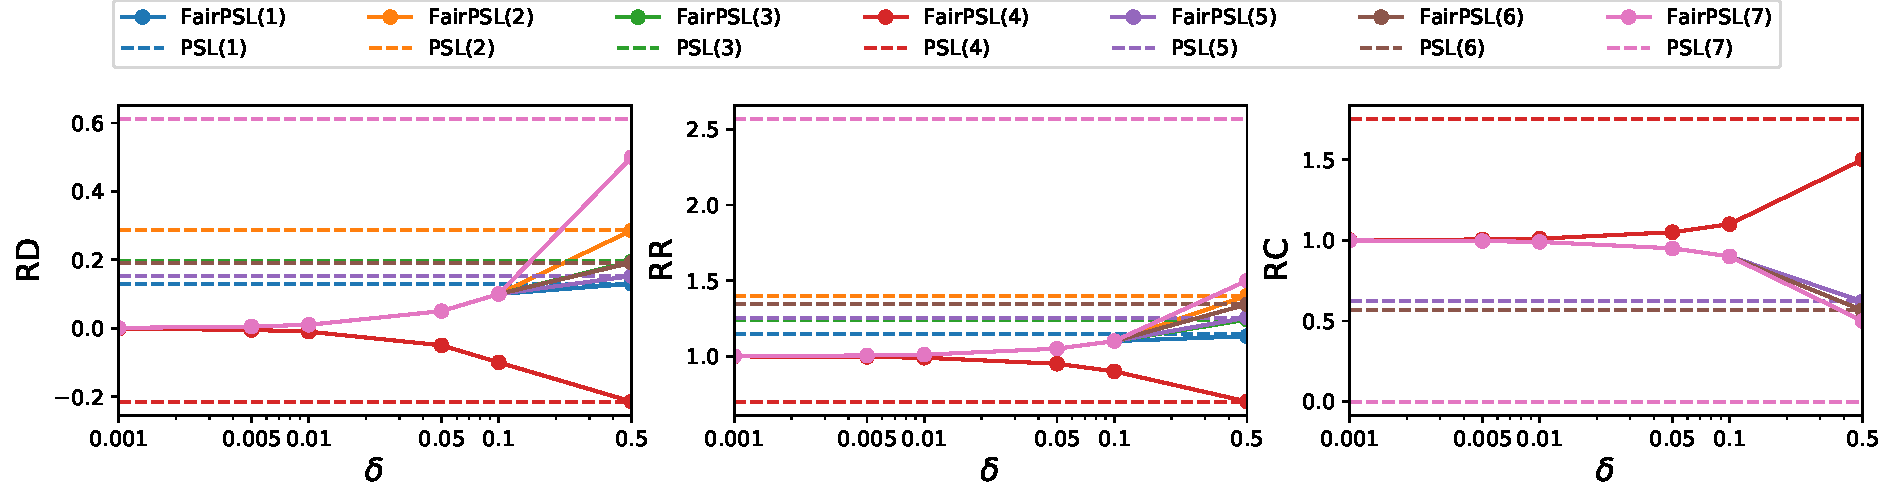
\includegraphics[width=1\linewidth]{figs/results_vis_uni_params.pdf}
\caption{\small Fairness score of predictions obtained by MAP inference of PSL and FairPSL, according to the fairness measures \emph{RD}, \emph{RR}, and \emph{RC}. The labels of datasets are mentioned with parenthesis next to the inference method. The FairPSL values of each measure are obtained by adding the $\delta$-fairness constraint of that measure.\label{fig:results}
}  
\end{figure}

To answer \textbf{Q1}, we run the MAP inference algorithm of PSL and FairPSL on seven synthetic datasets. 
We run the MAP inference of FairPSL multiple times on each dataset: For each of the three fairness measures, we add the corresponding $\delta$-fairness constraint with five thresholds $\{0.001, 0.005, 0.01, 0.05, 0.1, 0.5\}$.

Figure~\ref{fig:results} shows the fairness score of predictions in terms of the three fairness measures. As expected, tighter $\delta$-fairness constraints lead to better scores. Note that the best possible score according to RD is 0, as it computes a difference. Since RR and RC compute ratios, the best possible score according to these measures is 1. In our experiments, with any of these measures, taking $\delta = 0.001$ pushes the score of predictions to its limit.  

The $\delta$-fairness constraints modify the optimization problem of MAP inference by reducing the feasible region to solutions that conform with fairness guarantees. Research question \textbf{Q2} is concerned with the effect of this reduction on the accuracy of predictions. Note that decision quality is the same as the accuracy of predictions. To answer this question, we compare the inferred values for the decision atoms \textit{ToPromote(e)} against their actual values. These values are extracted from the known values of \textit{IsQualified(e)} according to rules 11 and 12 in Table~\ref{tab:pslmodel}. Figure~\ref{fig:accuracy} shows the area under the curve of the receiver operating characteristic~(AUC) of predicting the decision variable in three groups, namely the protected group, the unprotected group (i.e., promotion of the employees who have in-group managers), and all employees. By doing so, we make sure that our fairness constraints do not propagate bias towards either of the populations. Since the results of FairPSL with $\delta$-fairness constraints RR and RC are very similar to the results of RD, we only report the latter here.


\begin{figure}
    \centering
    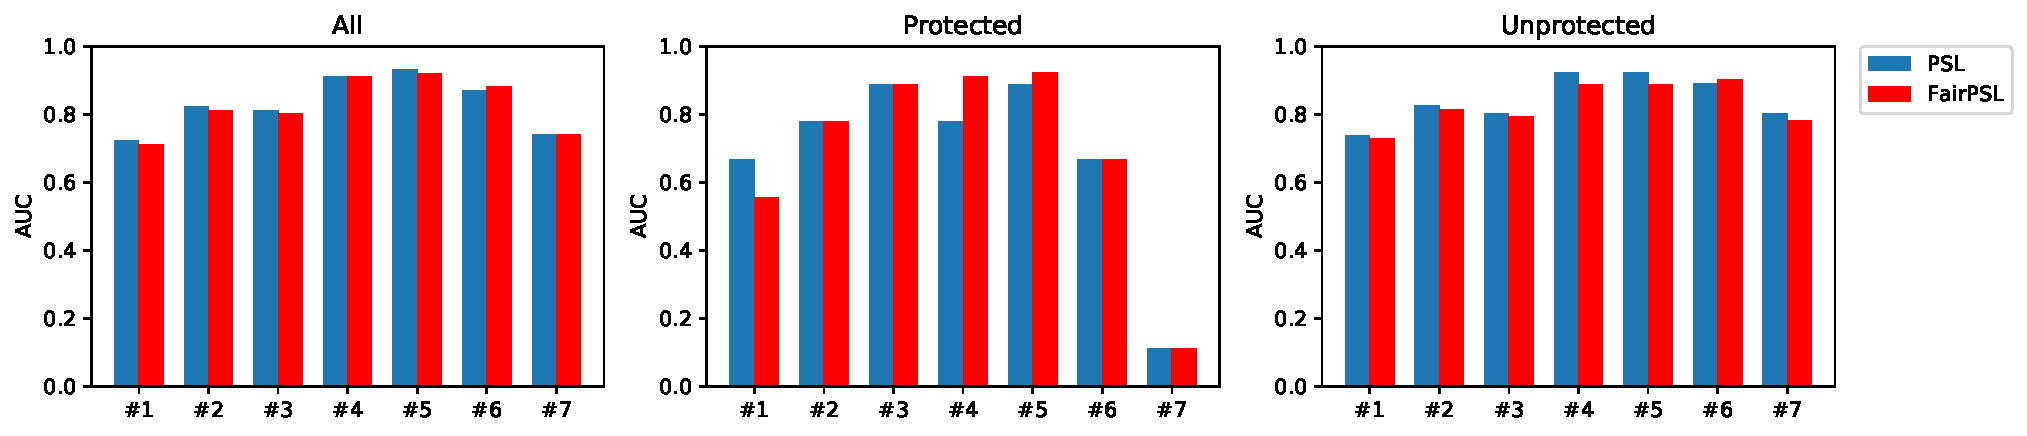
\includegraphics[width=\textwidth]{figs/roc.pdf}
    \caption{\small AUC score of predictions for truth values of unknown atoms \textit{ToPromote(e)} using MAP inference of PSL and FairPSL with $\delta$-fairness constraints $RD$ with $\delta=0.001$.}
    \label{fig:accuracy}
\end{figure}

According to Figure~\ref{fig:accuracy}, the results of both PSL and FairPSL in all seven datasets are close to each other. Note that although fairness may impose a cost in terms of overall accuracy, FairPSL often improves the accuracy of the protected class. Sometimes the overall predictions of FairPSL are even slightly better than PSL (e.g., dataset 6 and 7). As expected, the accuracy of the fourth setting where the opinions are unbiased are similar in both PSL and FairPSL. We observe that prediction of MAP inference for both FairPSL and PSL are similar, thus, in these settings at least, FairPSL guarantees fairness without hurting accuracy. Further investigation is required on the effect of the various ranges of discrimination (i.e., $\theta_1$, $\theta_2$, $\theta_3$, $\theta_4$) on the prediction results of FairPSL.



We also generate various types of organizations in which labels are not uniformly distributed, e.g., one population only occurs at the bottom levels of an organization. While we did not observe any differences in the behavior of our method with respect to accuracy and fairness measure, we found that the degree of discrimination is higher in such organizations. Further investigations on the structure of an organization on discrimination is an interesting direction for future research. 

\section{Conclusion and Future Directions}
\label{sec:conclusion}
Many applications of AI and machine learning affect peoples' lives in important ways. While there is a growing body of work on fairness in AI and ML, it assumes an individualistic notion of fairness.   In this paper, we have proposed a general framework for relational fairness which includes both a rich language for defining discrimination patterns and an efficient algorithm for performing inference subject to fairness constraints. We show our approach enforces fairness guarantees while preserving the accuracy of the predictions. 

There are many avenues for expanding on this work. For example, here we assumed that the discriminative pattern is given, however an automatic mechanism to extract discriminatory situations hidden in a large amount of decision records is an important and required task. Discrimination discovery has been studied for attribute-based fairness~\cite{pedreschi2013discovery}. An interesting next step is discrimination pattern discovery in relational data.

\section*{Acknowledgements}
This work is supported by the National Science Foundation under Grant Numbers CCF-1740850 and IIS-1703331. Golnoosh Farnadi and Behrouz Babaki are  supported by postdoctoral scholarships from IVADO through the Canada First Research Excellence Fund (CFREF) grant.

\begin{thebibliography}{10}
\itemsep=1pt 
\begin{small}

\bibitem{EUlaw}
European union legislation. (a) racial equality directive, 2000; (b) employment
  equality directive, 2000; (c) gender employment directive, 2006; (d) equal
  treatment directive (proposal), 2008.

\bibitem{UKlaw}
{UK} legislation. (a) sex discrimination act, 1975, (b) race relation act,
  1976.

\bibitem{USlaw}
United nations legislation. (a) universal declaration of human rights, 1948,
  (c) convention on the elimination of all forms of racial discrimination,
  1966, (d) convention on the elimination of all forms of discrimination
  against women, 1979.

\bibitem{alshukaili:iswc16}
Duhai Alshukaili, Alvaro A.~A. Fernandes, and Norman~W. Paton.
\newblock Structuring linked data search results using probabilistic soft
  logic.
\newblock In {\em International Semantic Web Conference {(1)}}, volume 9981 of
  {\em Lecture Notes in Computer Science}, pages 3--19, 2016.

\bibitem{bach:jmlr17}
Stephen~H. Bach, Matthias Broecheler, Bert Huang, and Lise Getoor.
\newblock Hinge-loss markov random fields and probabilistic soft logic.
\newblock {\em Journal of Machine Learning Research}, 18:109:1--109:67, 2017.

\bibitem{barocas2016big2}
Solon Barocas and Andrew~D Selbst.
\newblock Big data's disparate impact.
\newblock {\em California Law Review}, 104:671, 2016.

\bibitem{boyd2014networked}
Danah Boyd, Karen Levy, and Alice Marwick.
\newblock The networked nature of algorithmic discrimination.
\newblock In {\em Data and discrimination: Collected essays}, pages 53--57.
  2014.

\bibitem{brewer1979group}
Marilynn~B Brewer.
\newblock In-group bias in the minimal intergroup situation: A
  cognitive-motivational analysis.
\newblock {\em Psychological bulletin}, 86(2):307, 1979.

\bibitem{brewer2007social}
Marilynn~B Brewer.
\newblock The social psychology of intergroup relations: Social categorization,
  ingroup bias, and outgroup prejudice.
\newblock {\em Social Psychology: Handbook of Basic Principles}, 2007.

\bibitem{chouldechova2017fair2}
Alexandra Chouldechova.
\newblock Fair prediction with disparate impact: {A} study of bias in
  recidivism prediction instruments.
\newblock {\em CoRR}, abs/1703.00056, 2017.

\bibitem{dwork2012fairness3}
Cynthia Dwork, Moritz Hardt, Toniann Pitassi, Omer Reingold, and Richard~S.
  Zemel.
\newblock Fairness through awareness.
\newblock In {\em {ITCS}}, pages 214--226. {ACM}, 2012.

\bibitem{ebrahimi:emnlp16}
Javid Ebrahimi, Dejing Dou, and Daniel Lowd.
\newblock Weakly supervised tweet stance classification by relational
  bootstrapping.
\newblock In {\em {EMNLP}}, pages 1012--1017. The Association for Computational
  Linguistics, 2016.

\bibitem{farnadi2018fairness}
Golnoosh Farnadi, Behrouz Babaki, and Lise Getoor.
\newblock Fairness in relational domains.
\newblock In {\em AAAI/ACM Conference on AI, Ethics, and Society (AIES)}, pages
  108--114. ACM, 2018.

\bibitem{feldman2015certifying2}
Michael Feldman, Sorelle~A. Friedler, John Moeller, Carlos Scheidegger, and
  Suresh Venkatasubramanian.
\newblock Certifying and removing disparate impact.
\newblock In {\em {KDD}}, pages 259--268. {ACM}, 2015.

\bibitem{getoor2007introduction}
Lise Getoor and Ben Taskar.
\newblock {\em {Introduction to Statistical Relational Learning}}.
\newblock MIT press Cambridge, 2007.

\bibitem{hardt2016equality3}
Moritz Hardt, Eric Price, and Nati Srebro.
\newblock Equality of opportunity in supervised learning.
\newblock In {\em {NIPS}}, pages 3315--3323, 2016.

\bibitem{kamishima2011fairness}
Toshihiro Kamishima, Shotaro Akaho, and Jun Sakuma.
\newblock Fairness-aware learning through regularization approach.
\newblock In {\em ICDMW}, pages 643--650. {IEEE} Computer Society, 2011.

\bibitem{kouki:recsys15}
Pigi Kouki, Shobeir Fakhraei, James~R. Foulds, Magdalini Eirinaki, and Lise
  Getoor.
\newblock Hyper: {A} flexible and extensible probabilistic framework for hybrid
  recommender systems.
\newblock In {\em RecSys}, pages 99--106. {ACM}, 2015.

\bibitem{counterfactualfairness}
Matt~J. Kusner, Joshua~R. Loftus, Chris Russell, and Ricardo Silva.
\newblock Counterfactual fairness.
\newblock In {\em {NIPS}}, pages 4069--4079, 2017.

\bibitem{Pedreschi:2012}
Dino Pedreschi, Salvatore Ruggieri, and Franco Turini.
\newblock A study of top-k measures for discrimination discovery.
\newblock In {\em {SAC}}, pages 126--131. {ACM}, 2012.

\bibitem{pedreschi2013discovery}
Dino Pedreschi, Salvatore Ruggieri, and Franco Turini.
\newblock The discovery of discrimination.
\newblock In {\em Discrimination and Privacy in the Information Society},
  volume~3 of {\em Studies in Applied Philosophy, Epistemology and Rational
  Ethics}, pages 91--108. Springer, 2013.

\bibitem{ridgeway2004unpacking}
Cecilia~L Ridgeway and Shelley~J Correll.
\newblock Unpacking the gender system: A theoretical perspective on gender
  beliefs and social relations.
\newblock {\em Gender \& society}, 18(4):510--531, 2004.

\bibitem{sridhar:bioinformatics16}
Dhanya Sridhar, Shobeir Fakhraei, and Lise Getoor.
\newblock A probabilistic approach for collective similarity-based drug-drug
  interaction prediction.
\newblock {\em Bioinformatics}, 32(20):3175--3182, 2016.

\bibitem{verma2018fairness2}
Sahil Verma and Julia Rubin.
\newblock Fairness definitions explained.
\newblock In {\em 2018 IEEE/ACM International Workshop on Software Fairness
  (FairWare)}, pages 1--7. IEEE, 2018.

\bibitem{west2014exploiting}
Robert West, Hristo~S. Paskov, Jure Leskovec, and Christopher Potts.
\newblock Exploiting social network structure for person-to-person sentiment
  analysis.
\newblock {\em {TACL}}, 2:297--310, 2014.

\bibitem{zafar2017parity}
Muhammad~Bilal Zafar, Isabel Valera, Manuel Gomez{-}Rodriguez, Krishna~P.
  Gummadi, and Adrian Weller.
\newblock From parity to preference-based notions of fairness in
  classification.
\newblock In {\em {NIPS}}, pages 228--238, 2017.

\bibitem{zemel2013learning}
Richard~S. Zemel, Yu~Wu, Kevin Swersky, Toniann Pitassi, and Cynthia Dwork.
\newblock Learning fair representations.
\newblock In {\em {ICML} {(3)}}, volume~28 of {\em {JMLR} Workshop and
  Conference Proceedings}, pages 325--333. JMLR.org, 2013.

\end{small}
\end{thebibliography}

\end{document}

\end{article}

\makeatletter
\renewcommand{\AB@affillist}{}
\renewcommand{\AB@authlist}{}
\setcounter{authors}{0}
\makeatother

\begin{article}
{$SUQ^{2}$: Uncertainty Quantification Queries over Large Spatio-temporal Simulations}
{Noel Moreno Lemus, Fabio Porto, Yania M. Souto, Rafael S. Pereira, Ji Liu, Esther Pacciti, and Patrick Valduriez}
\graphicspath{{submissions/fabio/}}
%% 
%% Copyright 2007, 2008, 2009 Elsevier Ltd
%% 
%% This file is part of the 'Elsarticle Bundle'.
%% ---------------------------------------------
%% 
%% It may be distributed under the conditions of the LaTeX Project Public
%% License, either version 1.2 of this license or (at your option) any
%% later version.  The latest version of this license is in
%%    http://www.latex-project.org/lppl.txt
%% and version 1.2 or later is part of all distributions of LaTeX
%% version 1999/12/01 or later.
%% 
%% The list of all files belonging to the 'Elsarticle Bundle' is
%% given in the file `manifest.txt'.
%% 
%% Template article for Elsevier's document class `elsarticle'
%% with harvard style bibliographic references
%% SP 2008/03/01

%\documentclass[preprint,12pt,oneside,onecloumn]{elsarticle}
\documentclass[11pt]{article}
%% Use the option review to obtain double line spacing
%% \documentclass[authoryear,preprint,review,12pt]{elsarticle}

%% Use the options 1p,twocolumn; 3p; 3p,twocolumn; 5p; or 5p,twocolumn
%% for a journal layout:
%% \documentclass[final,1p,times,authoryear]{elsarticle}
%% \documentclass[final,1p,times,twocolumn,authoryear]{elsarticle}
%% \documentclass[final,3p,times,authoryear]{elsarticle}
%% \documentclass[final,3p,times,twocolumn,authoryear]{elsarticle}
%% \documentclass[final,5p,times,authoryear]{elsarticle}
%% \documentclass[final,5p,times,twocolumn]{elsarticle}

%% For including figures, graphicx.sty has been loaded in
%% elsarticle.cls. If you prefer to use the old commands
%% please give \usepackage{epsfig}

%% The amssymb package provides various useful mathematical symbols
%\usepackage{deauthor,times,graphicx}
%\usepackage{times,graphicx}

%\usepackage{amssymb, mathtools, bm}
%\usepackage{float}
%\usepackage{algorithm}
%\usepackage{multirow}
%\usepackage[noend]{algpseudocode}
%\usepackage{graphicx}
%\usepackage{multicol}
%\usepackage{hyperref}
%\usepackage{biblatex}
%\usepackage{authblk}
%\graphicspath{{./figs/}}
%\usepackage{subfig}

%\usepackage[belowskip=-15pt,aboveskip=0pt]{caption}
%\setlength{\intextsep}{10pt plus 2pt minus 2pt}

\begin{document}


\title{\textit{SUQ}$^2$: Uncertainty Quantification Queries over Large Spatio-temporal Simulations}

\author[a]{Noel Moreno Lemus  }
\author[a]{Fabio Porto }
\author[a]{Yania M. Souto  }
\author[a] {Rafael S. Pereira }
\author[c]{Ji Liu}
\author[b]{Esther Pacciti}
\author[b]{Patrick Valduriez }
\affil[a]{LNCC, DEXL, Petropolis, Brazil}
\affil[b]{Inria and LIRMM, University of Montpellier, France}
\affil[c] {Big Data Laboratory, Baidu Research, Beijing, China}


\maketitle

\begin{abstract}
The combination of high-performance computing
towards Exascale power 
and numerical techniques enables exploring complex physical phenomena using large-scale spatio-temporal modeling and simulation. The improvements on the fidelity of phenomena simulation require more sophisticated uncertainty quantification analysis, leaving behind measurements restricted to low order statistical moments and moving towards more expressive probability density functions models of uncertainty. In this paper, we consider the problem of answering uncertainty quantification queries over large spatio-temporal simulation results. We propose the $SUQ^2$ method based on the Generalized Lambda Distribution (GLD) function. GLD fitting is an embarrassingly parallel process that scales linearly to the number of available cores on the number of simulation points. Furthermore, the answer of queries is entirely based on computed GLDs and the corresponding clusters, which enables trading the huge amount of simulation output data by 4 values in the GLD parametrization per simulation point.
The methodology presented in this paper becomes an important ingredient in converging simulations improvements to the Exascale computational power. 


\end{abstract}



%% main text
\section{Introduction}
\label{introduction}
The rapid growth of high-performance computing combined with recent advances in  numerical techniques increases the accuracy of numerical simulations.
This leads to practical applicability in models for predicting the behavior of weather, hurricane forecasts \cite{Tobergte2013} and  subsurface hydrology \cite{Baroni2014a}, just to name a few, positioning simulations as increasingly important tools for high-impact predictions and decision-making applications.

In order to reach higher simulation accuracy
of reproduced phenomena, the scientific community is leaving behind the traditional deterministic approach, which  offers  point predictions with no associated uncertainty \cite{Johnstone2015},  to move towards Uncertainty Quantification (\textit{UQ}) as a common practice over simulation results analysis. Arguing for improvements in simulation accuracy, by the assessment of uncertainty quantification of simulation results consider the extra knowledge a scientist acquires whenever the simulation behaviours become more evident over different scenarios. The increase in simulation scenarios call for more computing power.
In a subsurface seismic domain, for example, a simulation computes the wave velocity at each point of an area. A scientist is interested in a particular region of the space where a salt dome is located. She may issue a query filtering only that spatial region and checking how precise is the velocity field in that area. In order to achieve that, she could quantify the uncertainty involved in the region of interest. This type of simulation that evaluates the uncertainty by analyzing its output is referred to as \emph{forward propagation}.
In this paper, we focus on answering uncertainty quantification queries over large spatio-temporal simulations $(UQ^2STS)$.  
The $UQ^2STS$ problem is challenging as: (1) it requires analyzing large amounts of simulation output data; (2) the uncertainty at each point may exhibit patterns too complex to be captured  by low order statistical moments (such as mean and standard deviation); (3) the uncertainty behavior may vary along a simulation spatio-temporal region leading to a complex data pattern to be modelled and an uncertainty expression of difficult interpretation. Thus, the problem involves conceiving a method to accurately and efficiently solve the $UQ^2STS$.

We propose the SUQ$^2$ method to solve this problem. SUQ$^2$ is based on the adoption of the generalized lambda distribution (\textit{GLD}) PDF type as a model of the uncertainty at each simulation computation point, which solves issue (2). Its uniform representation reduces significantly the computation of the necessary fitting function. Furthermore, by adopting a single function type, we could run clustering algorithms on the GLD parametrization, electing a representative data distribution for a large set of simulation points. This represents a huge saving in data storage, which solves issue (1). Finally, the cluster representatives are used to composed a mixture of GLDs  and to measure the information entropy of the $UQ^2STS$, which solves issue (3).  We illustrate the adoption of the SUQ$^2$ method with a case study in seismology. 

In our previous work \cite{Liu2019}, we designed a system to efficiently compute PDFs in large saptial datasets. The system implements a Spark dataflow to streamline the huge amount of PDF fitting computation. Our work extends the results of this work by adopting the GLDs as a generic model for data distribution, avoiding testing for different distribution types and uniformizing the computation of mixed PDFs in spatial-temporal regions. 

To the best of our knowledge, the first effort to use the \textit{GLD} to model uncertainty in data is the work of Lampasi et. al. \cite{Lampasi2006}, followed by Movahedi et. al. \cite{Movahedi2013} for a  task involving the computation of results reliability. The adoption of mixture of \textit{GLDs} is motivated by the work of Ning et. al. \cite{Ning2008}. Algorithms to use the mixture of \textit{GLDs} to model datasets have been deployed with the \textbf{GLDEX} R package.
Wellmann et al. \cite{Wellmann2012} propose to use information entropy as an objective measure to compare and evaluate model and observational results. Our SUQ$^2$ method combines these techniques.

The rest of the paper is organized as follows: Section \ref{UQBackground} gives the problem formalization and introduces the \textit{GLD} function.  Section \ref{Approach} presents the SUQ$^2$ method and the workflow to solve the $UQ^2STS$ problem. Section \ref{Experiments} gives an experimental evaluation
with a use case in seismology.
Section \ref{Conclusions} concludes.


\section{Preliminaries}
\label{UQBackground}
In this section we define some basic concepts needed for the rest of the paper. We first formalize the problem. Next, we present the Generalized Lambda Distribution function, including a discussion on its shape and the mixture of GLDs.

A simulation is a combination of a numerical method implementing a mathematical model and a discretization that enables to approximate the solution in points of space-time. A simulation can be used for two different types of problems: \textit{forward} or \textit{inverse}. \textit{Forward problems} study how uncertainty propagates through a mathematical model. In a simulation, a spatio-temporal domain is represented by a grid of positions $(s_{i},t_{j}) \in \mathcal{S} \times \mathcal{T}\subseteq\mathbb{R}^{3}\times\mathbb{R}$, where values of a quantity of interest \textit(QoI), such as velocity, are computed. In a parameter sweep application, a simulation is executed multiple times, each with a different initial configuration, leading to multiple occurrences for a given domain position, in order to explore the simulation behavior under different scenarios.

A simulation can be formally expressed as $\bm{q}=\mathcal{M}(\bm{\theta})$ where:  $\bm{\theta} \in \mathbf{R^{n}} $ is a vector of  input parameters of the model; $\mathcal{M}$ is a computational model, and $\bm{q} \in \mathbf{R^{k}}$ is a vector that represents  quantities of interest (\textit{QoI}). In a \textit{forward problem}, the parameters $\bm{\theta}$ are given and the quantities of interest $\bm{q}$  need to be computed. In stochastic models, at least one parameter is assigned to a probability density function (\textit{PDF}) or it is related to the parameterization of a random variable (\textit{RV}) or field, causing $\bm{q}$  to become a random variable as well.


In order to estimate a stochastic behavior of the output solution $\bm{q}$  in terms of input uncertainties $\bm{\theta}$, sampling methods analyze the values of $\mathcal{M}(\bm{\theta})$ at multiple sampled conditions in the $\Theta$ space (called stochastic space) directly from numerical simulations. Methods like Monte Carlo \textit{(MC)} are used to randomly sample in the stochastic space, and hence many sample calculations are required to achieve a convergence of stochastic estimations. As a result, the method returns multiple realizations of $\bm{q}$. Then, other methods to measure the uncertainty need to be applied.

In a more general case, the computational model $\bm{q}=\mathcal{M}(\bm{\theta})$ represents the spatio-temporal evolution of a complex systems, and the \textit{QoI} $\bm{q}$ can be represented as
$ \mathbf{Q} = (\mathbf{q}(s_{1},t_{1}),\mathbf{q}(s_{2},t_{2}),...,\mathbf{q}(s_{n},t_{n}))  
$, where: $(s_{1},t_{1}),(s_{2},t_{2}),....,(s_{n},t_{n}) \in \mathcal{S} \times \mathcal{T}\subseteq\mathbb{R}^{3}\times\mathbb{R}$ represents a set of distinct spatio-temporal locations, and
$\mathbf{q}(s_{i},t_{j})$ represents a value of the \textit{QoI} at the spatio-temporal location $(s_{i},t_{j})$.


In a stochastic problem, on each spatio-temporal location $(s_{i},t_{j})$ we have many realizations of $q(s_{i},t_{j})$ that can be represented as a vector $<q(s_{i},t_{j})>$. In this context, it is frequent that more than $10^4$ simulations are performed while exploring the model parameter space, which leads the output dataset to have a size of order  $N_{s}\times N_{t}\times N_{sim}$, where $N_{s}$ is the number of spatial locations, $N_{t}$ is the number of time steps, and $N_{sim}$ is the number of simulations.  An example of the volume of data generated by these simulations is given in the experimental evaluation (see Section \ref{Experiments}), where the output dataset is about 2.4 TB.

A simple approach to solve a spatio-temporal UQ query is to consider a simple aggregation query, computing the mean and standard deviation on the selected spatio-temporal region. This approach, albeit being simple and fast, is unable to capture  patterns exhibited by the data distribution of complex phenomena. The solution we propose in \cite{Liu2019} adopts probability density function (PDF) as a more accurate modeling data distribution at each point. However, the adoption of PDFs brings its own challenges. First, as the uncertainty may vary in different regions of the simulation, one needs to try multiple function types, such as Gaussian, Logarithm, Exponential, $etc$, at each spatial position to find the one closest to its data distribution. This leads to a huge computation cost for each simulation spatial position. Moreover, as a region may be defined by different PDF types, answering solving a
$(UQ^2STS)$ requires dealing with heterogeneous function types, making it more costly and harder to interpret the results. Thus, at the basis of the $SUQ^2$ method is the adoption of the GLD PDF type, which is presented in the next section. 

\subsection{Generalized Lambda Distribution}
\label{materials_methods}

The Generalized Lambda Distribution (GLD) has been applied to fitting phenomena in many fields with very good results. It was proposed by Ramberg and Schmeiser in 1974 \cite{Ramberg1974} as an extention of the Tukey's distribution, and it is tuned to represent different data distributions through the specification of $\lambda$ parameter, where $\lambda_{1}$ and $\lambda_{2}$ determine location and scale parameters, while $\lambda_{3}$  and $\lambda_{4}$ determine the skewness and kurtosis of the $GLD(\lambda_{1},\lambda_{2},\lambda_{3},\lambda_{4})$. The Ramberg and Schmeiser proposal is known as \textit{RS} parameterization.
The \textit{RS} parametrization has some constraints with respect to the values of  $(\lambda_{3}, \lambda_{4})$, see \cite{Karian2011}. To circumvent those constraints, Freimer et al. \cite{Freimer1988} introduced a new parameterization called \textit{FKML}: $Q_{FMKL}(y|\lambda_{1}, \lambda_{2}, \lambda_{3}, \lambda_{4})=\lambda_{1}+\frac{1}{\lambda_{2}}\left[\frac{y^{\lambda_{3}}-1}{\lambda_{3}} - \frac{(1-y)^{\lambda_{4}}-1}{\lambda_{4}} \right] $. As in the previous parameterization, $\lambda_{1}$ and $\lambda_{2}$ are the location and scale parameters, but in this one $\lambda_{3}$ and $\lambda_{4}$ are the tail index parameters. The advantage over the previous parameterization is that there is only one constraint on the parameters, i.e. $\lambda_{2}$ must be positive. 

Both representations (i.e. \textit{RS} and \textit{FMKL}) can present a wide variety of shapes and therefore are utilized in practice; however, generally the \textit{FMKL GLD} is preferred due to the ease in its use \cite{Corlu2016}. In this paper, we opt for using the \textit{FMKL GLD} representation.


\subsubsection{Shapes of GLD}
\label{gldShape}
A \textit{GLD} can describe a variety of shapes, such as U-shaped, bell shaped, triangular, and exponentially \cite{Su2007}. At the same time it provides good fits to many well know distributions. 

These \textit{GLD} properties are important to the  $SUQ^2$ method for two reasons. First, no previous knowledge is needed to fit the \textit{GLD} to a dataset. Second, \textit{GLDs} can be comparatively assessed; grouped based on their shapes, which enables running clustering algorithms, electing a representative distribution, and synthesizing the data in a cluster.

The shape of a \textit{GLD} depends on its $\lambda$ values. In the case of the \textit{FMKL GLD} parameterization, Freimer et al. \cite{Freimer1988} classify the shapes into five categories depending on the variety of distributions, which can be represented by several combinations of the shape parameters $\lambda_{3}$ and $\lambda_{4}$. 

The ability to model different shapes is critical to the $SUQ^2$ approach as it is the basis for the clustering algorithms (see Section \ref{Clusterizing the GLD based in its lambda values}).

\subsubsection{GLD mixture}
\label{GLDMixture}
In general, a \textit{mixture distribution} is the probability distribution of a random variable that is derived from a collection of other random variables. Given a finite set of \textit{PDFs} $\{p_{1}(x),p_{2}(x),\ldots,p_{n}(x)\}$, and weights $\{w_{1},w_{2},\ldots,w_{n}\}$ such that $w_{i} \geq 0$ and $\sum w_{i}=1$, the mixture distribution can be represented by writing the density $f(x)$ as a sum (which is a convex combination): $f(x)=\sum_{i}^n w_{i}p_{i}(x)$. Extending this concept to \textit{GLD}, the mixture distribution can be represented as:
$f(x)=\sum_{i}^n w_{i}GLD_{i}(\lambda_{1},\lambda_{2},\lambda_{3},\lambda_{4})$. This model is used in Section \ref{sub:gldMixtureWorkflow} to characterize the uncertainty in a spatio-temporal region.


\section{Simulation Uncertainty Quantification Querying (SUQ$^2$)}
\label{Approach}

In a stochastic problem, on each spatio-temporal location $(s_{i},t_{j})$ we have many realizations of $q(s_{i},t_{j})$. A schema to store this information in a relational database can be:
\begin{equation}\label{eq:data_base_structure}
S(s_{i},t_{j},simId,q(s_{i},t_{j}))
\end{equation}
where $simId$ represents the \textit{id} of one simulation (realization).

In this section, we first show how to fit a GLD to a spatio-temporal dataset. Next, we present the clustering of GLDs using the lambda parameters. Then, we present how to compute the uncertainty in a region using a mixture of GLDs and information entropy.
Figure \ref{fig:workflow} shows the $SUQ^2$ method represented by a workflow and divided into three main steps: fitting process, clustering and UQ analysis.

\subsection{Fitting a GLD to a spatio-temporal dataset}
\label{gldFitProcess}
Given a random sample $q_{1}, q_{2}, q_{3},...,q_{n}$, the basic problem in fitting a statistical distribution to these data is the distribution from which the sample was obtained. In our approach we divide this process into three steps: (1) fiting the \textit{GLD} to the data; (2) validating the resulting \textit{GLD}; (3) evaluating the quality of the fit.

Algorithm \ref{alg:fitGLD} realizes Step 1. Before starting the fitting process, we need to group all the simulation values that correspond to the same spatio-temporal location $(s_{i},t_{j})$.  As a result, we get a new dataset $S^*(s_{i},t_{j},<q_1,q_2,..,q_n>)$, where $q_i, 1 \le i \le n$, represents a vector of all the values of $q$ at point $(s_{i},t_{j})$. This process is efficiently computed according to the approach developed in \cite{Liu2019}.

For each spatio-temporal location $(s_{i},t_{j}) \in \mathcal{S} \times \mathcal{T}$, we use a function of the GLDEX R package \cite{Su2007}, to fit the \textit{GLD} to a vector $<q_1,q_2,..,q_n>$, line 2. This is an embarrassingly parallel computation method, which we adopt in \cite{Liu2019}.

Once the fitting process in Step 1 has been applied, a fitted GLD is associated to each simulation spatio-temporal position. The schema in Equation \ref{eq:data_base_structure} is modified to accommodate the GLD parameters in place of the list of simulation values: $S(s_{i},t_{j},GLD_i,j(\lambda_1,\lambda_2,\lambda_3,\lambda_4))$.

Finally, we need to evaluate the fit quality, which assesses whether the
\textit{GLD} probability density function (PDF) correctly describes the dataset. We use here the Kolmogorov-Smirnov test (KS-test), that determines if two datasets differ significantly. In this case, the datasets are the original dataset and a second one generated using the fitted GLD. As a result, this test returns the p-value, line 5.
%of Algorithm \ref{alg:fitGLD}. 
If the p-value is bigger than 0.05, lines 6-7, 
%of Algorithm \ref{alg:fitGLD},
we store the lambda values of those \textit{GLDs}.


\begin{algorithm} 
%\vspace{-2cm}
\caption{Fitting the GLD to a spatio-temporal dataset}\label{alg:fitGLD}
\begin{algorithmic}[1] 
\Function{gldFit}{$S(s_{i},t_{j},<q_1,q_2,...,q_n>)$} 
\State $<\lambda_{1},\lambda_{2},\lambda_{3},\lambda_{4}> \gets \Call {fit.gld.lm}{<q_1,q_2,...,q_n>}$

\State $isValid_{(s_{i},t_{j})} \gets \Call {validityCheck}{<\lambda_{3},\lambda_{4}>}$
\If{$isValid_{(s_{i},t_{j})}$}
\State $[pvalue,D]_{(s_{i},t_{j})} \gets \Call{ks}{<\lambda_{1},\lambda_{2},\lambda_{3},\lambda_{4}>_{(s_{i},t_{j})}}$
\EndIf
\If{$pvalue_{(s_{i},t_{j})} > 0.05$}
\State $\Call{storeLambdas}{<\lambda_{1},\lambda_{2},\lambda_{3},\lambda_{4}>,s_{i},t_{j}}$
\EndIf
\EndFunction 
\end{algorithmic} 
\end{algorithm} 

\subsection{Clustering the GLD based on its lambda values}
\label{Clusterizing the GLD based in its lambda values}
In Section \ref{gldShape}, we discussed the two most important parameterizations of the \textit{GLD} and selected \textit{FMKL} to be used for the rest of the  paper. In this parametrization, $\lambda_{1}$ represents the location of the \textit{GLD} and is directly related to the mean of the distribution. $\lambda_{2}$ is the scale, directly related to the standard deviation, and $\lambda_{3}$ and $\lambda_{4}$ represent the left and right tails of the distribution. Combinations of $\lambda_{3}$ and $\lambda_{4}$ can be used to estimate the skewness and kurtosis of the distribution.

As $\lambda_{2}$ defines the dispersion, and $\lambda_{3}$ and $\lambda_{4}$ the shape of a \textit{GLD}, the combination of these parameters determine the quantification of the uncertainty, from the \textit{GLD} point of view.


According to Lampasi et al. \cite{Lampasi2006}, a particular $GLD(\lambda_{1},\lambda_{2},\lambda_{3},\lambda_{4})$ can be rewritten as: 

\begin{equation}\label{eq:rewrite_gld}
GLD(\lambda_{1},\lambda_{2},\lambda_{3},\lambda_{4}) = \lambda_{1} + \frac{1}{\lambda_{2}}GLD(0,1,\lambda_{3},\lambda_{4}) 
\end{equation}

In Equation \ref{eq:rewrite_gld}, the first term applies $\lambda_1$ while the second involves the remaining parameters.
Then, we can apply clustering algorithms only considering parameters in the second term: $\lambda_{2}$, $\lambda_{3}$ and $\lambda_{4}$. The clustering algorithm would be applied in two steps \ref{alg:fitGLD}. The first clusters based on the $\lambda_2$ values, according to the curve dispersion. Next, for each cluster obtained in the first step, we cluster again according to parameters $\lambda_{3}$ and $\lambda_{4}$, which are the parameters that define the shape of the distribution.


\begin{algorithm} 
%\vspace{-2cm}
\caption{Clustering the GLD based on its $\lambda_{(2,3,4)}$ values.}\label{alg:clusterGLD}
\begin{algorithmic}[1] 
\Function{gldClustering}{$S(s_{i},t_{j}, <0,\lambda_{2},\lambda_{3},\lambda_{4}>)$} 
\State $S(s_{i},t_{j}, clusterID_{I}) \gets \Call {firstStep}{S(s_{i},t_{j},\lambda_{2})}$
\For{\textbf{each} $clusterID_{I}$}
\State $S(s_{i},t_{j}, clusterID_{II}) \gets \Call {secondStep}{S(s_{i},t_{j},<\lambda_{3},\lambda_{4}>), S(s_{i},t_{j}, clusterID_{I})}$
\EndFor
\EndFunction 
\end{algorithmic} 
\end{algorithm} 

Then, in this step of our workflow, we cluster the \textit{GLDs} using $\lambda_{2}$, $\lambda_{3}$ and $\lambda_{4}$ values. The final result of this step is:
\begin{equation}
S_{\mathcal{C}}(s_{i},t_{j},GLD_{k},clusterID)
\end{equation}
where
$clusterID$ represents the ID of the cluster to which the \textit{GLD} at the spatio-temporal location $(s_{i},t_{j})$ belongs. With the domain modeled by clustered \textit{GLDs}, we can use this result to characterize the uncertainty in a particular spatio-temporal region or to measure numerically the corresponding uncertainty. In Sections \ref{sub:gldMixtureWorkflow} and \ref{sub:InfomationEntropyRegionWorkflow}, we describe how these approaches are implemented (see Figure \ref{fig:workflow}).

\subsection{Use of GLD mixture to characterize uncertainty in a spatio-temporal region}
\label{sub:gldMixtureWorkflow}
One of the main advantages of assessing the complete probability distribution of the outputs is that we can use the \textit{PDFs} to answer queries. If we consider that the clustering of GLD has good quality, we can pick the GLD at the centroid of each cluster as a representative of all its members. In this context, in a particular spatio-temporal region, each cluster may be qualified with a weight given by:$ w_{k}=\frac{1}{N}\sum_{i=1}^S \sum_{j=1}^T w(s_{i},t_{j})$, where: $w(s_{i},t_{j}) =
  \begin{cases}
    1 & \text{if $clusterID(s_{i},t_{j}) = k$} \\
    0 & \text{otherwise}
  \end{cases}$ and  \textit{N} is the number of points in the region $(\mathcal{S}_{i} \times \mathcal{T}_{j})$.

The weight $w_k$ is the frequentist probability of occurrence of the cluster \textit{k} in the region, and complies with the conditions defined in Section \ref{GLDMixture} that $w_{k} \geq 0$ and $\sum w_{k}=1$.

Remember that the mixture of the GLDs can be written as $f(x)=\sum_{k=1}^K w_{k}GLD(\lambda_{1},\lambda_{2},\lambda_{3},\lambda_{4})$. So, if we have the weights and a representative GLD for each cluster, we have the mixture of GLD that characterizes the uncertainty in the spatio-temporal region $(\mathcal{S}_{i} \times \mathcal{T}_{j})$. The GLD mixture process is summarized in 
Algorithm 3, which receives  a spatio-temporal region and a \textit{clusterId}  associated to each spatio-temporal point. In the main loop, lines 3 to 5, the algorithm increments the number of occurrences for each clusterId and the total number of points. At line 7, the mixture expression is returned.


%Algorithm \ref{alg:mixGLD}.
\begin{figure}
%\vspace{-2cm}
    \centering
    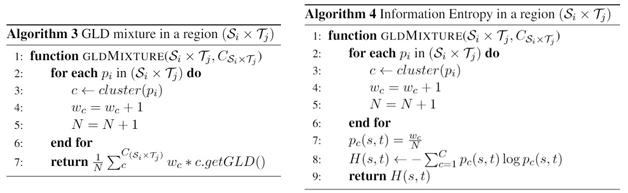
\includegraphics{figs/Algorithms_3_4.png}
\end{figure}

\subsection{Information entropy as a measure of uncertainty in a spatio-temporal region}
\label{sub:InfomationEntropyRegionWorkflow}
Now, what happens if we want to measure the uncertainty quantitatively? The information entropy is useful in this context. We use the different clusters we got in Section \ref{Clusterizing the GLD based in its lambda values} as the different outcomes of the system. The information entropy is computed as follows $H(s,t)=-\sum_{c=1}^C p_{c}(s,t)\log p_{c}(s,t)$, where $c$ represent a particular cluster in the set of clusters $C$, and $p_{c}(s,t)$ represents the probability of occurrence of the cluster $c$ in the spatio-temporal region $(s,t)$.

Algorithm 4 computes the information entropy in a region $C_{(\mathcal{S}_{i} \times \mathcal{T}_{j})}$. In lines 2 to 7, we assess the probability of each cluster in the region. Using this result, we can evaluate the information entropy $H(s, t)$, line 8, and finally, return the result in line 9.


\begin{figure}[!ht]
%\vspace{-1cm}
    \centering
    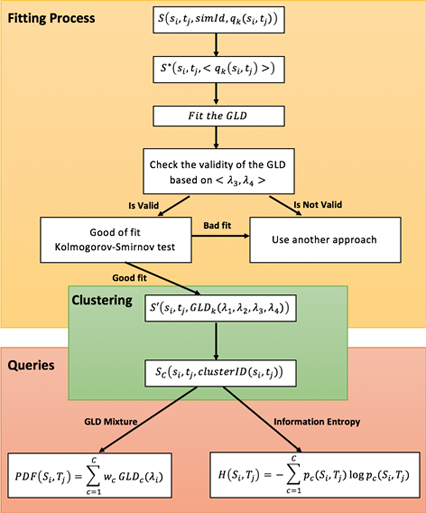
\includegraphics{figs/Diagram.png}
    \caption{SUQ$^2$ workflow divided into three steps, (a) fitting process, (b) clustering of the GLDs and, (c) queries over the results of the clustering process.}
    \label{fig:workflow}
\end{figure}

\section{Experimental Evaluation}
\label{Experiments}
In this section, we first introduce the data used in our experiments. Next, we discuss how we apply the fitting and clustering techniques over the experiment dataset. Then, we present the queries used in the performance evaluation and discuss the results expressed as a mixture of GLDs and values computed using information entropy.

As a case study, we use the HPC4e seismic benchmark, a collection of four 3D models and sixteen associated tests  \footnote{The benchmark can be freely downloaded from https://hpc4e.eu/downloads/} to generate the data of a cube. The models include simple cases that can be used in the development stage of any geophysical imaging practitioner as well as extremely large cases that can only be solved in a reasonable time using supercomputers. The models are generated based on the required size by means of a Matlab/Octave script. The tests can be used to benchmark and compare the capabilities of different and innovative seismic modelling approaches, thus simplifying the task of assessing the algorithmic and computational advantages.



\subsection{Dataset}
In the HPC4e benchmark, the models are designed as sets of 16 layers with constant physical properties. The top layer delineates the topography and the other 15 delineate different layer interface surfaces or horizons. To generate a single cube with dimensions $250\times501\times501$ we can use the values provided in the benchmark. For example, to generate a cube in the $v_{p}(m/s)$ variable we can use the fixed values of Table \ref{tab:valuesOfVp}. The first slice of this cube is shown in Figure \ref{fig:slice1}.

\begin{table}[ht]
\parbox{.45\linewidth}{
\begin{center}
    \begin{tabular}{|l|l|l|l|l|}
    \hline
    \textbf{Layer} & $v_{p}(m/s)$ &   \textbf{Layer} & $v_{p}(m/s)$ \\ \hline
    1     & 1618.92 &  9 & 2712.06\\ \hline
    2     & 1684.08 &  10 & 2532.2\\ \hline
    3     & 1994.35 &  11 & 2841.03\\ \hline
    4     & 2209.71 &   12 & 3169.31\\ \hline
    5     & 2305.55 &   13 & 3169.31\\ \hline
    6     & 2360.95 &  14 & 3642.28\\ \hline
    7     & 2381.95 &   15 & 3659.22\\ \hline
    8     & 2223.41 &   16 & 4000.00\\ \hline
    \end{tabular}
    \caption {Values of $v_{p}$ used in the generation of a single velocity field cube.}
    \label{tab:valuesOfVp}
    \end{center}
%\quad
}
%\end{table}
\parbox{.45\linewidth}{
%\begin{table}[ht]
\begin{center}
\resizebox{0.6\columnwidth}{!}{
    \begin{tabular}{|l|l|l|l|l|l|}
    \hline
    \textbf{Layer} & \textbf{PDF Family} & \textbf{Parameters} & \textbf{Layer} & \textbf{PDF Family}& \textbf{Parameters} \\\hline
    1     & Gaussian & [1619, 711.2] & 9     & Exponential & [3949, 394.9]             \\ \hline 
    2     & Gaussian & [3368, 711.2] & 10   & Exponential & [5983, 711.2]               \\ \hline
    3     & Gaussian & [8839, 711.2] & 11   & Exponential & [3520, 352.0]              \\ \hline
    4     & Gaussian & [7698, 301.5] & 12   & Exponential & [3155, 315.5]              \\ \hline
    5     & Lognormal   & [7723, 294.7] &  13   & Uniform     & [2541, 396.4]              \\ \hline
    6     & Lognormal   & [7733, 292.2] & 14   & Uniform     & [2931, 435.3]              \\ \hline
    7     & Lognormal   & [7658, 312.1] & 15   & Uniform     & [2948, 437.0]             \\ \hline
    8     & Lognormal   & [3687, 368.7] & 16   & Uniform     & [3289, 471.1]              \\ \hline
   \end{tabular}
}
    \caption {PDFs and the parameters used to sample the $v_{p}$ attribute, to generate n velocity models.}
    \label{tab:PDFsOfVp}
    \end{center}
}
\end{table}

As our purpose is to study the uncertainty in the simulation output, we need the input $v_{p}(m/s)$ to present a stochastic behavior. We model the input according to the distributions depicted in Table \ref{tab:PDFsOfVp}. Next, using a Monte Carlo method, we generate a sampling of 1000 realizations of the $v_{p}(m/s)$ variable and use a Matlab script provided by the HPC4e benchmark to generate the cube data. We perform the simulations
1000 times, one for each  realization, and generate 1000 cubes (230 GB) as output. The generated cubes are $250\times501\times501$  multi-dimensional arrays. In order to simplify the computational process and visualize the results, we select the slice 200
to be used in our experiments.
Then, we have 1000 realizations of a slice with size of $250\times501$. The data schema in Equation \ref{eq:data_base_structure} can be simplified as we only have two spatial dimensions and no time domain. Thus, the dataset can be represented as $S(x_{i},y_{j},simId,v_{p}(x_{i},y_{j}))$. In this new representation, $(x_{i},y_{j})$ is the 2D coordinates and $v_{p}(x_{i},y_{j})$ is the velocity value at point $(x_{i},y_{j})$. \textit{simId} represents the Id of the simulation, ranging from 1 to 1000.


\subsection{Fitting the GLD}\label{ft_gld}
The first step is to find the \textit{GLD} that best fits the dataset at each spatial location. Running Algorithm \ref{alg:fitGLD}, we get a new 2D array:
\begin{equation}\label{eq:gld_fit_2D}
S'(x_{i},y_{j},GLD(\lambda_{1}, \lambda_{2}, \lambda_{3}, \lambda_{4}))
\end{equation}
The raw data is significantly reduced and the new dataset is characterized by four lambda values at each spatial location. 

To check how good is the fit, we use the \textit{ks.test} algorithm included in the R-package \textit{stats} \cite{Lopes2011}, which return the \textit{p-value} at each spatial location. Our results show that the fit of the GLD is acceptable in most cases (\textit{p-value} $>0.05$),
%to be more exact, 
in 82 \% of the spatial locations (see Figure \ref{fig:p_values_greater_05}). In the 18\% regions where the GLD modeling was not acceptable, some \textit{GLD} extensions proposed in \cite{Karian2011} could be used. Since the main purpose of this paper is to demonstrate the usefulness of the \textit{GLD} in \textit{UQ}, this particular problem is beyond our scope.

\begin{figure*}[!ht]
\begin{multicols}{2}
    \centering
    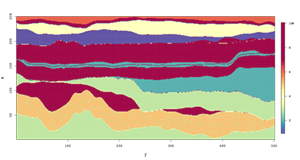
\includegraphics{figs/clusters_slice.png}
    \caption{One slice of the $250\times501\times501$ cube. In the slice, we can distinguish between the different layers.}
    \label{fig:slice1}
    \centering
    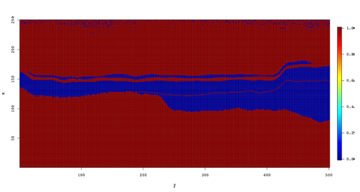
\includegraphics{figs/p_value_greater_05.png}
    \caption{The red color shows where the p-value is greater than 0.05.}
    \label{fig:p_values_greater_05}
\end{multicols}
\end{figure*}

\subsection{Clustering}\label{useCaseClustering}
Up to now, the dataset is characterized by the schema depicted by Equation \ref{eq:gld_fit_2D}. Then, using a clustering algorithm, such as k-means, we group the GLDs based on its $(\lambda_{2}, \lambda_{3}, \lambda_{4})$ values, as discussed in Section \ref{Clusterizing the GLD based in its lambda values}.
In this paper, we use the k-means algorithm with $k=10$. The choice of the clustering algorithm and the parameterization is subject for further investigation and is beyond the scope of this paper.

Once the clustering algorithm is applied, a new dataset is produced. In the new dataset,  for each spatial location, a label indicates the cluster the \textit{GLD} belongs to, as shown (see the schema at Equation \ref{eq:clustersresult}) in Figure \ref{fig:clusters}. Note that in Figure \ref{fig:clusters}, the blue region corresponding to cluster 11 is not a cluster itself. It is rather the region where the \textit{GLD} is not valid (see Section \ref{ft_gld}).

\begin{equation}\label{eq:clustersresult}
S_{\mathcal{C}}(x_{i},y_{j},clusterID, GLD_{x_{i},y_{j}})
\end{equation}

\begin{figure*}[!ht]
%\vspace{-2cm}
\begin{multicols}{2}
    \centering
        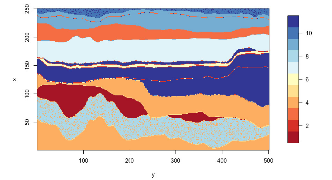
\includegraphics{figs/clusters_image.png}
    \caption{Result of the clustering using k-means with
    $k=10$.}
    \label{fig:clusters}
    \centering
    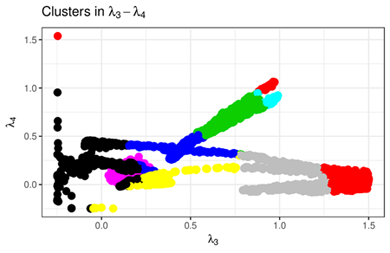
\includegraphics{figs/clusters_l3_l4.png}
    \caption{Distribution of the clusters in the $(\lambda_{3}, \lambda_{4})$ space. The points that belongs to a same cluster are one near the others, as was expected.}
    \label{fig:clusters_lambda3_lambda4_space}
\end{multicols}
\end{figure*}


If we visually compare Figure \ref{fig:slice1} with Figure \ref{fig:clusters}, we observe a close similarity. 

Another interesting result is shown in Figure \ref{fig:clusters_lambda3_lambda4_space}, where we plot the clusters in $(\lambda_{3}, \lambda_{4})$ space. As we mentioned in Section \ref{gldShape}, the shape of the \textit{GLD} depends on the values of $\lambda_{3}$ and $\lambda_{4}$. In this scenario, the expected result is that the members of the same cluster share similar values of $\lambda_{3}$ and $\lambda_{4}$. This is exactly the result we can observe in Figure \ref{fig:clusters_lambda3_lambda4_space}. 

To further corroborate this fact, Figure \ref{fig:cluster1} shows the \textit{PDFs} of 60 members of the 10 clusters. Visually assessing the figures gives an idea of how similar are the shapes of the members of a same cluster and how dissimilar are the shapes of the  members of different clusters. This suggests that our approach is valid. A product of these observations is that we can pick one member of each cluster (the centroid) as a representative of all the members of this cluster, Table \ref{tab:center_of_the_clusters}. The selected member is going to be used to answer the queries in the next Sections.
\begin{table}[ht]
\begin{center}
    \begin{tabular}{|l|l|l|l|l|l|l||l|}
    \hline
    \textbf{Cluster} & $\lambda_{2}$ & $\lambda_{3}$ & $\lambda_{4}$ & \textbf{Cluster} & $\lambda_{2}$ & $\lambda_{3}$ & $\lambda_{4}$  \\ \hline
    1     & 0.0013937313 & 0.9585829 & 1.04696461   &   6 & 0.0003894541 & 1.4076354 & -0.01925743 \\ \hline
    2     & 0.0005291388 & 1.1633978 & -0.07162550  &  7 & 0.0021972784 & 0.3253562 & 0.01493809 \\ \hline
    3     & 0.0020630696 & 0.1349486 & 0.17305941   &  8 & 0.0015421749 & 0.9491101 & 0.86699555 \\ \hline
    4     &  0.0016238358 & 0.8653824 & 0.83857646  &  9  & 0.0018672401 & 0.2176002 & 0.17862024  \\ \hline
    5     & 0.0027346929 & 0.5084664 & 0.39199164  &  10   & 0.4856397733 & 0.1404140 & 0.14011298  \\ \hline
    \end{tabular}
 \caption {Clusters centroids.}
 \label{tab:center_of_the_clusters}
 \end{center}
\end{table}

%\vspace{-5cm}
\begin{figure}[!ht]
%\vspace{-2cm}
    \centering
    %\includegraphics[scale=0.3]{figs/clusters2_s.png}
    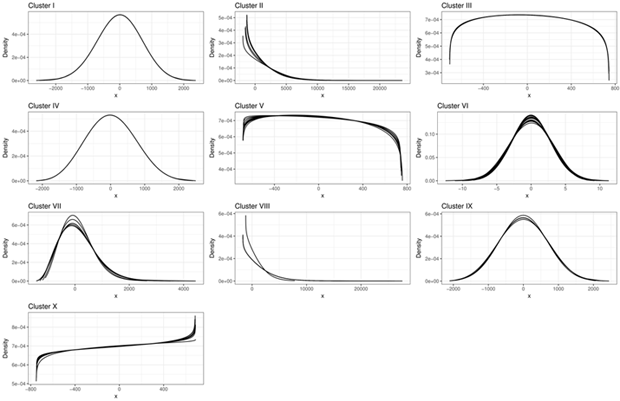
\includegraphics{figs/clusters2.png}
    \caption{\textit{PDFs} of 60 members of the 10 clusters obtained using k-means over the $(\lambda_{2}, \lambda_{3}, \lambda_{4})$ values.}
    \label{fig:cluster1}
%\end{figure}
%\vspace{0.5cm}

%\begin{figure*}
\begin{multicols}{2}
    \centering
    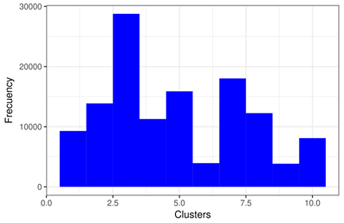
\includegraphics[scale=0.5]{figs/Clusters_histogram.png}
    %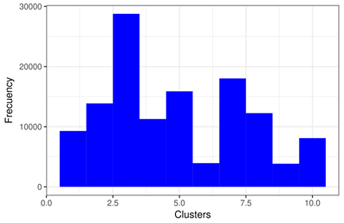
\includegraphics[bb 0 0 794 515]{figs/Clusters_histogram.png}
    \caption{Distribution of the 125250 points by clusters.}
    %\label{fig:clusters}
    \centering
    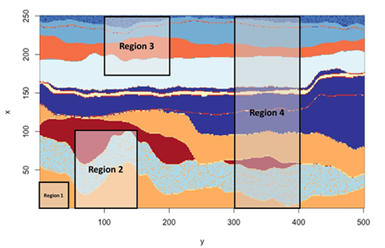
\includegraphics{figs/regions_queries.png}
    \caption{Analysis Regions. The four regions where selected intentionally in this way to warranty different distributions of the clusters inside it.}
\end{multicols}
\end{figure}

The 125250 points of the slice are distributed through the clusters following the histogram of Figure 7.

\subsection{Spatio-temporal queries}
Up to this point, the initial dataset is summarized as depicted by the schema in Equation \ref{eq:clustersresult}. It can be used to answer queries and validate our approach, by comparing the results with the raw data.

First of all, we select four spatio-temporal regions of the dataset where the clusters suggest us different behaviors. The regions are shown in Figure 8. 
With these four regions, we assess the adoption of the \textit{GLD} mixture to obtain the \textit{PDF} that characterizes the uncertainty in a specific  region (see Sections \ref{GLDmixtureresults} and \ref{informationEntropyresults}). We use the information entropy to assign a value that measures the uncertainty at each region. In Section \ref{GLDmixtureresults}, we expect the GLD mixture to characterize well the raw data, and in Section \ref{informationEntropyresults}, we hope that the information entropy is zero in region 1 and increases between regions 2, 3 and 4.

\subsubsection{GLD mixture}\label{GLDmixtureresults}
In this experiment, we use the representative \textit{GLDs} at each cluster and the weight associated to it in the region. Using these parameters, we can build a \textit{GLD mixture} that characterizes the uncertainty on that region. We use
Algorithm 3 described in Section \ref{GLDMixture}. First, we query the region to find  the clusters represented inside it, and how they are distributed. The retrieved results are shown in Table \ref{tab:distribution_of_the_clusters_by_regions}. If we divide the columns of Table \ref{tab:distribution_of_the_clusters_by_regions} by the sum of the elements of each column, we get the weight needed to formulate the \textit{mixed GLDs}. It is clear that the \textit{GLD} in region 1 is represented by the \textit{GLD} of cluster 4. In the other three cases, we get what is shown in the set of 
equations \ref{eq:gld_mix}.


\begin{table}[!ht]
%\vspace{-0.5cm}
\begin{center}
\scalebox{0.6}{
    \begin{tabular}{|l|l|l|l|l|}
    \hline
    \textbf{Cluster} & \textbf{Region 1} &  \textbf{Region 2} &  \textbf{Region 3} &   \textbf{Region 4}  \\ \hline
    1     & 0   		& 2250 & 0 & 979            \\ \hline
    2     & 0   		& 0 & 0 & 268           \\ \hline
    3     & 0      	& 0 & 2596 & 1468       \\ \hline
    4     & 1640	& 4467 & 0 & 5173         \\ \hline
    5     & 0       & 149 & 0 & 269          \\ \hline
    6     & 0     & 0 & 0 & 416           \\ \hline
    7     & 0       & 0 & 1967 & 3920           \\ \hline
    8     & 0     & 3335 & 0 & 3432             \\ \hline
    9     & 0      & 0 & 1918 & 3280       \\ \hline
    10   & 0      & 0 & 901 & 583         \\ \hline
    \end{tabular}}
    \caption {Distribution of the clusters by regions. The four regions are selected intentionally this way to warrant different distributions of the clusters inside it.}
    \label{tab:distribution_of_the_clusters_by_regions}
    \end{center}
\end{table}


\begin{align}
%\vspace{-0.2cm}
\begin{split}
\label{eq:gld_mix}
GLD_{region2} = 0.22GLD_{c1} + 0.44GLD_{c4} + 0.014GLD_{c5} + 0.33GLD_{c8} \\
 GLD_{region3} = 0.34GLD_{c3} + 0.26GLD_{c7} + 0.25GLD_{c9} + 0.12GLD_{c10} \\
 GLD_{region4} = 0.22GLD_{c1} + 0.44GLD_{c4} + 0.014GLD_{c5}  + 0.33GLD_{c8}
\end{split}
\end{align}


Now, we need to evaluate whether the \textit{mixture of GLDs} correctly models the uncertainty in a region. We perform the same \textit{ks-test} used to evaluate the
good quality of the fit, described in Section \ref{gldFitProcess}. Based on the \textit{p-value}, Table \ref{tab:p_values_by_regions}, we can conclude that in all 4 regions the \textit{mixture of GLDs} is a good fit to the raw data.

\begin{table}[ht]
\begin{center}
    \begin{tabular}{|l|l|l|l|l|}
    \hline
    \textbf{Metrics} & \textbf{Region 1} &  \textbf{Region 2} &  \textbf{Region 3} &   \textbf{Region 4}  \\ \hline
    p-value     & 0.73   		& 0.56 & 0.34 & 0.08            \\ \hline
    \end{tabular}
    \caption {p-values by regions.}
    \label{tab:p_values_by_regions}
    \end{center}
\end{table}



\subsubsection{Information Entropy}\label{informationEntropyresults}

Based on the distribution of clusters inside the regions (see Table \ref{tab:distribution_of_the_clusters_by_regions}), we can compute the entropy. 

\begin{table}[ht]
\begin{center}
    \begin{tabular}{|l|l|l|l|l|}
    \hline
    \textbf{entropy} & \textbf{Region 1} &  \textbf{Region 2} &  \textbf{Region 3} &   \textbf{Region 4}  \\ \hline
    value     & 0   		& 1.122243 & 1.41166 & 2.024246            \\ \hline
    \end{tabular}
    \caption {Information Entropy by regions.}
    \label{tab:entropy_by_regions}
    \end{center}
\end{table}

As we expect (see Table \ref{tab:entropy_by_regions}), the entropy in region 1 is zero, because the region contains only members of the cluster 4. On the other regions the entropy increases from region 2 to region 4, as expected. The information entropy is a very good and simple measure of the uncertainty, and here it is demonstrated its usefulness combined with the \textit{GLD}.

 

\section{Conclusion}
\label{Conclusions}

In this paper, we proposed SUQ$^2$, a method to answer uncertainty quantification (UQ) queries over large spatio-temporal simulations. SUQ$^2$ trades large simulation data by probability density functions (PDFs), thus saving huge amount of storage space and computational cost. It enables complex data distribution representation at each simulation point, as much as a  spatio-temporal view  of simulation uncertainty computed by mixing spatial point PDFs.
We evaluated SUQ$^2$ using a seismology use case, considering the computation of uncertainty in regions of a slice of the seismic cube. The results show that SUQ$^2$ method produces an accurate view of the uncertainty in regions of space-time while considerably saving storage space and reducing the cost associated with the PDF modeling of the dataset. To the best of our knowledge, this is the first work to use GLD as the basis for answering UQ queries in spatio-temporal regions and to compile a series of techniques to produce a query answering workflow.



\subsection*{Acknowledgments}
This work has been funded by CNPq, CAPES, FAPERJ, the Inria HPDaSc
and SciDISC Associated Teams and the European Commission (HPC4E H2020) project.


\itemsep=1pt
\begin{thebibliography}{10}
\begin{small}


\bibitem{Tobergte2013}
D. R. Tobergte and S. Curtis.
\newblock {Workshop on Quantification, Communication, and Interpretation of
  Uncertainty in Simulation and Data Science}.
\newblock in {\em Journal of Chemical Information and Modeling}, 53(9):1689--1699,
  2013.


\bibitem{Baroni2014a}
G. Baroni and S. Tarantola.
\newblock {A General Probabilistic Framework for uncertainty and global
  sensitivity analysis of deterministic models: A hydrological case study}.
\newblock in {\em Environmental Modelling and Software}, 51:26--34, 2014.

\bibitem{Johnstone2015}
R. H. Johnstone, E. T. Y. Chang, R. Bardenet, T. P. de~Boer,
  D. J. Gavaghan, P. Pathmanathan, R. H. Clayton, and G. R. Mirams.
\newblock {Uncertainty and variability in models of the cardiac action
  potential: Can we build trustworthy models?}
\newblock in {\em Journal of Molecular and Cellular Cardiology}, 96:49--62, 2016.
  


\bibitem{Karian2011}
Z. A. Karian and E. J. Dudewicz.
\newblock {\em {Handbook of fitting statistical distributions with R}}.
\newblock 2011.


\bibitem{Freimer1988}
M. Freimer, C. T. Lin, and G. S. Mudholkar.
\newblock {A Study Of The Generalized Tukey Lambda Family}.
\newblock in {\em Communications in Statistics - Theory and Methods},
  17(10):3547--3567, 1988.
  
\bibitem{Corlu2016}
C. G. Corlu and M. Meterelliyoz.
\newblock {Estimating the Parameters of the Generalized Lambda Distribution:
  Which Method Performs Best?}
\newblock in {\em Communications in Statistics: Simulation and Computation},
  45(7):2276--2296, 2016.
  

\bibitem{Su2007}
S. Su.
\newblock {Fitting Single and Mixture of Generalized Lambda Distributions to
  Data via Discretized and Maximum Likelihood Methods: GLDEX in R}.
\newblock {\em Journal of Statistical Software}, 21(9), 2007.

\bibitem{Lampasi2006}
D. A. Lampasi, F. Di Nicola, and L. Podesta.
\newblock {Generalized lambda distribution for the expression of measurement
  uncertainty}.
\newblock {\em IEEE Transactions on Instrumentation and Measurement},
  55(4):1281--1287, 2006.
  
\bibitem{Movahedi2013}
M. M. Movahedi, M. R. Lotfi, and M. Nayyeri.
\newblock {A solution to determining the reliability of products Using
  Generalized Lambda Distribution}.
\newblock {\em Research Journal of Recent Sciences Res.J.Recent Sci},
  2(10):41--47, 2013.
  
 \bibitem{Ning2008}
W. Ning, Y. Gao, and E. J. Dudewicz.
\newblock {Fitting mixture distributions using generalized lambda distributions
  and comparison with normal mixtures}.
\newblock {\em American Journal of Mathematical and Management Sciences},
  28(1-2):81--99, 2008.
  
\bibitem{Wellmann2012}
J. F. Wellmann and K. R. Lieb.
\newblock {Uncertainties have a meaning: Information entropy as a quality
  measure for 3-D geological models}.
\newblock {\em Tectonophysics}, 526-529:207--216, 2012.

\bibitem{Liu2019}
J. Liu,N. Lemus, E. Pacitti, F. Porto, P.  Valduriez. \newblock {Parallel computation of PDFs on big spatial data using spark}. \newblock in {em Distributed and Parallel Databases}, pp. 1-28. In press, 10.1007/s10619-019-07260-3, 2019.

\bibitem{Lopes2011}
R. H. C. Lopes  \newblock {Kolmogorov-Smirnov Test.} \newblock in {Lovric M. (eds) International Encyclopedia of Statistical Science. Springer, Berlin, Heidelberg}, 2011.

\bibitem{Ramberg1974} J. S. Ramberg, and B. W. Schmeiser.\newblock {An approximate
method for generating asymmetric random
variables}. \newblock in {em Communications of the ACM}, 17(2), 78–82.
doi:10.1145/360827.360840, 1974.


\end{small}
 \end{thebibliography}
\end{document}

\endinput
%%
%% End of file `elsarticle-template-harv.tex'.

\end{article}

\makeatletter
\renewcommand{\AB@affillist}{}
\renewcommand{\AB@authlist}{}
\setcounter{authors}{0}
\makeatother

\begin{article}
{Networking and Storage: The Next Computing Elements in Exascale Systems?}
{Alberto Lerner, Rana Hussein, Andre Ryser, Sangjin Lee, Philippe Cudre-Mauroux}
\graphicspath{{submissions/alberto/figs/}}
\documentclass[11pt,dvipdfmx]{article}

%\usepackage{deauthor}
%\usepackage{times}
%\usepackage{graphicx}

\newcommand{\softsubsec}[1]{\vspace{0.6em}\noindent\textbf{#1}}
\newcommand{\softsec}[1]{\vspace{1em}\noindent\textbf{#1}}

%\graphicspath{{./submissions/alberto/figs/}}

\begin{document}

\title{Networking and Storage: The Next Computing Elements in Exascale Systems?}

\author{Alberto Lerner$^1$~~~~Rana Hussein$^1$~~~~Andr\'{e} Ryser$^1$~~~~Sangjin Lee$^2$\thanks{Work done while visiting the University of Fribourg.}~~~~Philippe Cudr\'{e}-Mauroux$^1$  \vspace{0.4em} \\$^1$\emph{University of Fribourg~~~~~~~~~~~~$^2$Hanyang University} \\ \emph{Switzerland~~~~~~~~~~~~~~~~~~~~~~~~~~~~~South Korea}}

\maketitle

\begin{abstract}
Many large computer clusters offer alternative computing elements in addition to
general-purpose CPUs.
GPU and FPGAs are very common choices.
Two emerging technologies can further widen the options in that context: in-network
computing (INC) and near-storage processing (NSP).
These technologies support computing over data that is in transit between nodes
or inside the storage stack, respectively.
There are several advantages to moving computations to INC and NSP platforms.
Notably, the original computation path does not need to be altered to
route data through these subsystems; the network and the storage are naturally
present in most computations.


In this paper, we describe the evolutionary steps that led to INC and NSP platforms
and discuss how they can improve critical computing paths in large-scale
database systems.
In the process, we comment on the constraints that the current generation of
these platforms present as well as expose why we believe them to be relevant
to the next generation of exascale platforms.
\end{abstract}


\section{Motivation}
\label{sec:motivation}

\begin{figure}[t]
    \centering
    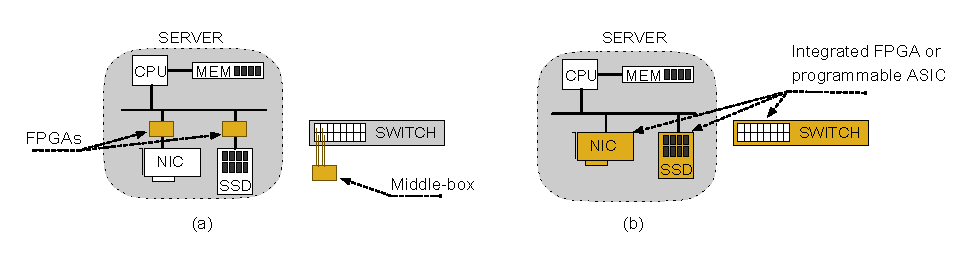
\includegraphics[bb=0 0 451 108]{fig_bump_internal.eps} %% 0.75
    \caption{Alternative in-network computing and near-storage processing
      platforms.
      (a) Using ``bump-in-the-wire'' FPGAs or network ``middle-boxes'' to create
      early application logic sites.
      (b) Leveraging programmability within the device for application logic.}
    \label{fig:bump_internal}
\end{figure}


The networking and storage stacks have always carried some computing power.
Network switches can triage billions of packets per second.
Solid-state drives (SSDs) can scramble and encode gigabytes of data per second
(for error correction purposes~\cite{cai17}).
Despite such computing power, applications have no access to how the
devices process the data, other than by issuing IO requests.
The functionality of these devices has been closed to changes.  Opening them
would require supporting a certain level of \emph{programmability}.


Nonetheless, the benefits of executing application logic close to networking and
storage devices are known~\cite{fang19, teubner13}.
New algorithms that take advantage of proximity to the data become viable and
provide both performance and power consumption gains.
Figure~\ref{fig:bump_internal}(a) illustrates how FPGAs and network
``middle-boxes'' can create these opportunities.


The lack of programmability in network and storage devices has impacted not
only applications.
It has also hindered the advancement of these platforms.
On the networking side, new protocols emerge that depend heavily on hardware to
run at high-speeds.
\emph{Fixed-function} devices, the ones that have their functionality ``baked''
into the hardware, may need to undergo a full, lengthy development cycle before
they can run new protocols.
Recently, a solution emerged where a new class of networking devices started
supporting programmability (e.g., in programmable switches~\cite{bosshart13} and
``smart'' NICs~\cite{zilberman14}).
The protocols these devices run are expressed as software programs.


The need for programmability also emerged on storage platforms recently.
SSDs are designed to shield applications from the intricacies of managing
flash memory.
However, evidence appeared that SSDs often miss the right performance decisions
because of the separation between it and the
applications~\cite{bjorling17}.
A more \emph{modular} SSD design, deemed \emph{open-channel}, was proposed that
allows a host (a server), rather than the SSD itself, to make certain low-level
decisions.
The modules that run on the host are software-based, therefore programmable.


Developers soon realized that the programmability could also be used by
applications.
It made it possible to inject application code directly into the networking and
storage stacks.
Figure~\ref{fig:bump_internal}(b) depicts such a scenario.
\emph{In-network computing} and \emph{near-storage processing} emerged as the
disciplines that leverage processing power in the network and storage stacks,
respectively, for application purposes.


An application that benefits from INC or NSP contains, by definition, algorithms
running in different computing elements of a system.
These algorithms ought to communicate at high speed.
The most commonly used interconnect for such systems has been based on the
PCIe bus standard~\cite{budruk03}.
At this time, the standard is being revised to operate at higher speeds.
PCIe is also being extended with mechanisms to support cache coherence protocols
to run atop of it~\cite{ccix19, cxl19}.


Despite their potential, INC and NSP platforms are not without challenges.
INC is a more mature technology with increasingly popular programmable models
that shield the developer from the intricacies of the devices.
Such programming models, however, are quite different from a general-purpose
CPU’s.
In contrast, NSP often uses general-purpose processors---but much less powerful
ones than server-class CPUs.
In both cases, porting algorithms to these platforms requires rethinking the
algorithms to fit either a different model or a less-powerful environment.


In this paper, we elaborate on the above challenges and opportunities of
adopting INC and NSP as platforms to improve application performance.
We summarize the contributions of this paper are as follows:
\begin{itemize}
  \setlength{\itemsep}{0pt}
  \setlength{\parsep}{0pt}
  \setlength{\parskip}{0pt}
  \setlength{\topsep}{0pt}
  \setlength{\partopsep}{0pt}
\item We discuss the evolution and recent advancements of INC and NSP platforms;
\item We present specific computation tasks that can benefit from them;
\item We describe the challenges that still remain in order to use INC and NSP
  as application platforms;
\item Finally, we present the benefits of adopting the current generation of INC
  and NSP.
\end{itemize}


The rest of this paper is structured as follows.
We discuss the programmability of the network and storage stacks in more detail
in Section~\ref{sec:background}.
We show examples of computing paths that can leverage INC and NSP capabilities in
Section~\ref{sec:data_paths}.
We comment on the evolution of the PCIe interconnect and the possibilities it
opens in Section~\ref{sec:interconnects}.
We discuss the challenges and opportunities of adopting INC and NSP platforms in
Section~\ref{sec:challenges}.
We elaborate on how ready for adoption the technologies are in
Section~\ref{sec:discussion}, before concluding in Section~\ref{sec:conclusion}.


\section{An Abridged History of INC and NSP}
\label{sec:background}

There have been many attempts to conciliate speed and flexibility in
networking hardware devices.
Figure~\ref{fig:evolution_net} depicts the main ideas behind the relevant
milestones in that context.


\begin{figure}[h]
  \centering
  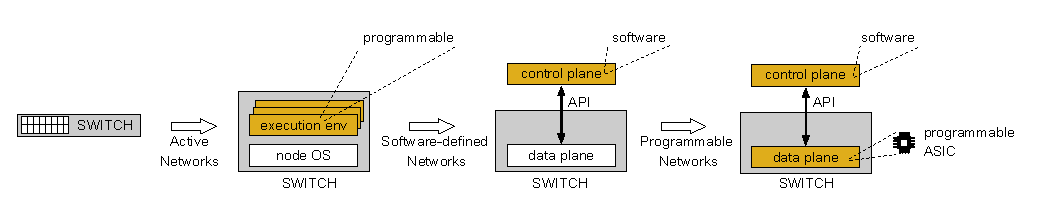
\includegraphics[bb=0 0 483 88]{fig_evolution_net.eps} %% 0.68
  \caption{Evolution of the network stack towards programmability.}
  \label{fig:evolution_net}
\end{figure}


\emph{Active Networks}, one of the first attempts, proposed a standard
architecture for more flexible network devices~\cite{calvert98}.
The goal of the architecture is to enable changes to the device
behavior—--typically to implement new protocols—--via the execution of
user-driven customization.
There are two main components in such a device.
First, a node operating system that manages basic IO functionality, including
processing, storage, and transmission.
Second, multiple Execution Environments (EE) that support the execution of
programs containing packet-processing logic.
Applications can inject code into the device through an API, which generates
special packets for the device to execute.
Active networks proved to be very flexible; however, they ran considerably
slower than their fixed-function counterparts.


\emph{Software-Defined Networks} (SDN), a later attempt at a more flexible
network, is also centered around a standard device
architecture~\cite{kreutz15}.
The main feature of the architecture is the separation of the control plane
(policy definition) from the data plane (policy implementation).
The control plane would contain information such as routing tables; the data
plane would use that information to forward packets without sacrificing speed.
An SDN device could adopt a new protocol if the SDN standard recognizes that
protocol.
Introducing new protocols, however, still required changes in the SDN standard
itself and sometimes also on the devices.
The main issue was that SDN only supports custom logic on the control plane.
Protocols that depended on special per-packet logic need to send these packets
to the control plane, which in turn processes them, pushing the results back to
the data plane.
The additional path cannot sustain \emph{line-rate}, as one calls the individual
port speed of a switch.


In a more recent development, \emph{Programmable Dataplanes} (also referred to
as \emph{Programmable Networks}) allowed custom logic on the data
plane~\cite{bifulco18}.
The cornerstone of this technology is a generation of programmable ASICs (chips)
that supports a certain degree of stateful packet processing without compromising
speed~\cite{bosshart13}.
This balance is captured by a programming model called Protocol Independent
Switch Architecture (PISA)~\cite{sivaraman16}.
PISA shields the programmer from various device intricacies and, because it was
designed to be protocol-independent, it proved adept at expressing application
computations as well.
Programmable networks created the conditions for a new generation of
applications to push specialized logic into the network, i.e., to perform
\emph{in-network computing}.


\vspace{1em}
We now turn our attention to the evolution of the storage stack.
Just as with networks, the idea of near-storage processing is not new, but the
driver for altering this stack has been more application-centric than in
networking.
In the early 2000s, a seminal proposal, called \emph{Active Disks}, gained
traction that aimed at transforming hard drive controllers into data-processing
platforms~\cite{riedel01}.
These controllers often carried a small, general-purpose processor that was
somewhat over-dimensioned for its purpose.
Applications could place logic on that processor, and access/modify the data
blocks that were streaming in and out of the hard drive.
The computing power of these controllers ultimately proved to be underwhelming,
and the industry saw little need to improve them.


Eventually, SSDs based on NAND-flash displaced hard drives in many applications.
Managing flash memory requires considerably more computing power than a magnetic
medium, and flash memory error rates are very high, which requires
computational-intensive error correction techniques~\cite{cai17}.
Moreover, the industry decided that SSDs should be drop-in replacements for hard
drives.
SSDs execute internally a compatibility layer called Flash Translation Layer
(FTL) for that purpose~\cite{chung09}.
All these factors turn SSDs into relatively powerful embedded devices.


A proposal soon emerged to leverage SSD controllers for database query
processing using \emph{smart SSDs}~\cite{do13}.
As with active disks, the computing capacity on early devices was not sufficient
for most computations in practice~\cite{do19}.
It would take a new generation of devices to accommodate fast database
logic~\cite{kim16}.
However, the industry focus was more on making devices faster than on making
them smarter.
Performance wasting was an issue, as the FTL not always makes the best decisions
from an application's point of view.
Some efforts emerged that tried to make SSD architectures more open to
configurations.
Figure~\ref{fig:evolution_ssd} captures the essential steps of this effort.


\begin{figure}[h]
  \centering
  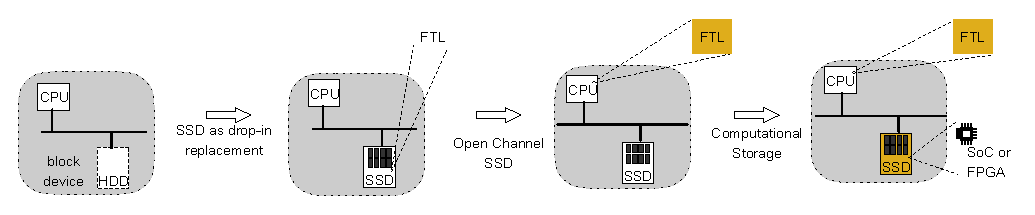
\includegraphics[bb=0 0 481 87]{fig_evolution_ssd.eps} %% 0.68
  \caption{Evolution of the storage stack towards programmability.}
  \label{fig:evolution_ssd}
\end{figure}

\emph{Open Channel SSDs} appeared from a growing understanding that many of the
FTL tasks were better performed leveraging application
knowledge~\cite{bjorling17}.
In an open-channel SSD, some of the FTL responsibilities are removed from the
device.
Instead, they run on the host housing the SSD or even inside individual
applications~\cite{ouyang14}.
Naturally, these devices expose a lower-layer view of the underlying flash
medium.


With more exposure to SSD architectural details, several works emerged to build
tooling around these devices.
These efforts range from frameworks to program SSD controllers~\cite{picoli20},
to performance measurement tooling~\cite{lerner20}, to even full SSD rapid
prototyping platforms~\cite{kwak20}.
At the same time, a class of works appeared that deploy application code on
SSDs, making them a \emph{Computational Storage} platform~\cite{picoli19, ruan19,
woods14}.
The common thread in these works is that they increase the existing computing
power of the devices by building them on platforms such as a System-on-a-Chip
(SoC) or an FPGA.
The tooling and the additional computing capacity paved the way for
\emph{Near-Storage Processing}.


One problem that remains open, however, is the lack of a consensus around a
programming model.
While there are recent proposals in that sense (e.g., in~\cite{gu16}), these
models leave many aspects undefined.
For instance, they have not addressed how to interface application logic with
internal device mechanisms.
An application that wishes to influence the IO scheduling policy of a device
directly has no means to do so.
There is also no consensus on how to shield an application developer from
specific aspects of different devices.


\section{Alternative Computing Paths}
\label{sec:data_paths}

INC and NSP  provide alternative sites beyond a CPU where applications can place
logic.
This fundamentally changes the traditional data movement patterns we see in
CPU-centric algorithms, potentially bringing performance and power savings
benefits.
We illustrate these possibilities in this section by presenting and discussing
several use cases in large-scale data management.


\subsection{In-Network Data Aggregation}
\label{ssec:aggr}

Data aggregation is a very common operation in data management.
Aggregation involves grouping data by specific criteria and calculating
summaries over each group.
A typical example is the \texttt{GROUP BY} clause in \texttt{SQL}.
When the data volume is large, the operation can involve several servers,
e.g., as in a rack-wide computation.
Figure~\ref{fig:flow_1}(a) illustrates one possible way to solve such a distributed
aggregation.


The servers agree on how to partition the data, taking into consideration the
grouping key.
This divides the work into disjoint, independent tasks.
Each server reshuffles its data while performing the aggregation over its
assigned partition, as data arrives.
Eventually, all the machines send their aggregation results to an elected
server, which combines them into a global result.
Note that throughout all these interactions, the switch performs data
transmissions only.


\begin{figure}[h]
    \centering
    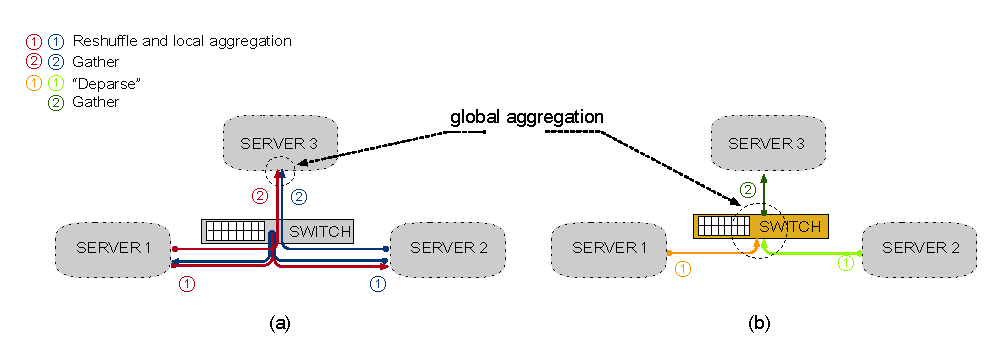
\includegraphics[bb=0 0 462 156]{fig_flow_1.eps} %% 0.75
    \caption{Data aggregation scenario (e.g., SQL GROUP BY).
      (a) With a ``passive'' switch, the servers first repartition the data
      and work on aggregating its assigned partition locally.
      Then, an elected server gathers all partitions and performs the global
      aggregation.
      (b) On an INC platform, an ``active'' switch can, in typical situations,
      perform the global aggregation in one step and transmit the results to an
      elected server.
      We use a given color to represent each unique data stream in the
      computation.
      }
    \label{fig:flow_1}
\end{figure}


In Figure~\ref{fig:flow_1}(b), we show that using the switch as an active
element simplifies the entire computing path~\cite{lerner19}.
We assume that the switch is programmable and that it can be leveraged to hold
an entire aggregation table.
The size of such a table is often manageable, as it is proportional to the
number of groups involved, rather than the size of the dataset.
Note that the servers need not reshuffle the data nor perform an aggregation on
a partition.
Because programmable switches perform computations at line-speed, the
aggregation table on the switch will be completed as soon as the last server
finishes transmitting its tuples, and can then be sent immediately to an elected
server.


Not all computations are suitable for INC deployment.
The important caveats include: (a) the number of steps the switch can execute
over each packet is limited; (b) the kind of instructions the switch can perform
is also constrained; and (c) programmable network devices adhere to a
programming model that imposes a \emph{forward logic}-style onto algorithm
design.
Loops and complex branching are strongly discouraged, although possible.
In practice, these restrictions reduce the choices of data structures the switch
can support.
In particular, the aggregation described in Figure~\ref{fig:flow_1}(b) requires
a hash table to be adapted to INC constraints.
In this case, the number of collisions can be handled on the switch up to a
certain bound.
Relaxing this constraint involves using a technique called
``overflowing''~\cite{lerner19}, which allows treating long collision chains
outside the switch without a noticeable performance penalty in most cases.

These limitations notwithstanding, a large class of computations can benefit from
INC platforms~\cite{ports19}.
Moreover, processing data on the switch tends to scale well as the number of
servers grows in the cluster.
The number of switches naturally grows with the number of servers.


\subsection{Near-Storage Checkpoint Derivation}
\label{ssec:cp_derivation}

We now describe an opportunity that arises specifically in an in-memory database
system.
Like most DBMSs, in-memory databases guarantee durability using a persistent
transaction log.
Because the log can get arbitrarily long, it would be impractical to recover
from a crash just by replaying it.
Therefore, databases also perform a periodical checkpoint (e.g., by taking a
snapshot) of the current memory state and write it to persistent storage, often
SSDs.
A recovery algorithm can load the snapshot and replay the portion of the log
acquired after the checkpoint.
In in-memory databases, the log and checkpoint are the only workloads written to
disk.


The logging and checkpointing processes compete for both disk and memory
bandwidth.
Figure~\ref{fig:flow_2}(a) shows these contention points.
The checkpointing process reads the database contents from the main-memory while
it is being queried/modified.
The checkpointing process also issues write requests to the SSD, which have to
be scheduled along with the logging workload.
The contention is responsible for the throughput reduction that many systems
experience during checkpoints.


\begin{figure}[h]
  \centering
  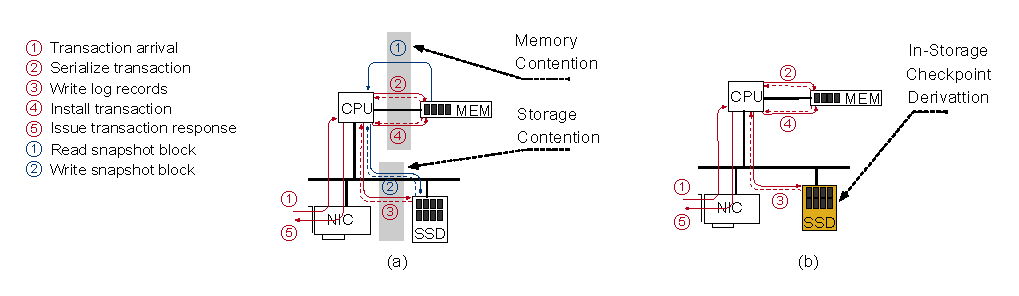
\includegraphics[bb=0 0 473 126]{fig_flow_2.eps} %% 0.75
  \caption{Checkpoint computation scenario.
    (a) Transaction logging (red) and checkpoint (blue) are two parallel
    processes.
    They compete for memory and disk bandwidth.
    (b) A checkpoint could be derived by processing the transaction log inside
    an SSD.
    The solid lines represent data; the dashed ones, control and/or return.
  }
  \label{fig:flow_2}
\end{figure}


The key observation here is that partial snapshots, which can serve as
checkpoints, can be derived from the log stream directly.
We believe that such derivations may very well occur inside a smart SSD.
We show in Figure~\ref{fig:flow_2}(b) that once we move that process to the
device, the contention points disappear.


Note, however, that the processing power on an SSD is far smaller than that of a
general-purpose CPU.
We cannot possibly expect to move the same algorithm we used on a CPU into an
NSP platform and obtain similar performance results.
Creating a checkpoint derivation algorithm for an SSD requires finding snapshot
approximations that the device can process at the necessary pace.
We comment on Section~\ref{sec:challenges} how specific architectural changes on
smart SSDs can make this task easier.


\subsection{Low Latency Database Replication}
\label{ssec:low_latency}


Another code path that can benefit from either INC or NSP is that of a replica
node in a database system.
On a master node, transactions need to be serialized via a concurrency control
algorithm.
The latter typically runs on a CPU.
The replica node code-path is simpler because the serial order of the
transactions was already determined.
The CPU takes the modifications coming from the network card and persists them
on disk in the same order it received them.
Subsequently, it updates its data structures and sends a notification to the
master node that it accepted the transaction.
Figure~\ref{fig:flow_3}(a) depicts such an interaction.


\begin{figure}[h]
  \centering
  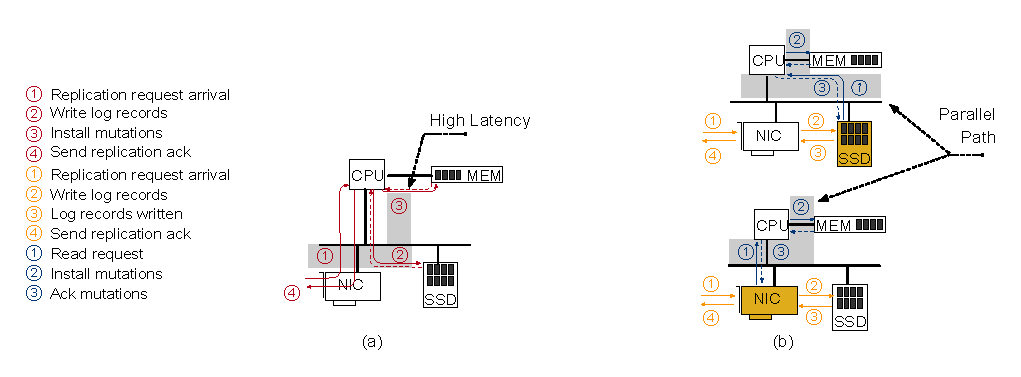
\includegraphics[bb=0 0 474 165]{fig_flow_3.eps} %% 0.75
  \caption{Database replica node scenario.
    (a) Each transaction log entry is first persisted in storage and then
    applied to memory, as the CPU coordinates the replication.
    (b) If an ``active'' NIC or SSD coordinates the process, the persistence and
    memory update paths can proceed in parallel.
  }
  \label{fig:flow_3}
\end{figure}


Note that the replica code path incurs in latency.
The master node may be withholding the original transaction until the
replication path is completed.
We can optimize this code path in at least two ways.
Using NSP, the NIC would send the modification stream directly to a smart SSD.
In turn, the SSD could be programmed to coordinate the interaction instead of
the CPU.
The SSD would notify the NIC after it persisted the changes, reducing the
latency.
It would also, in parallel, allow the CPU to read (and perform) the
modifications.
An alternative path exists where the NIC itself would perform the coordination.
Figure~\ref{fig:flow_3}(b) shows both cases.
This scenario involves having the NIC and the SSD communicate without any CPU
intervention.
This type of communication is called peer-to-peer DMA~\cite{budruk03} and it has
been used in other contexts before, such as direct access to a remote disk
(e.g., NVMe-over-Fabrics~\cite{guz18}).


\section{Upcoming Interconnects}
\label{sec:interconnects}

INC and NSP platforms rely on an interconnect to communicate with other
computing elements in a system.
PCIe has been the \emph{de facto} interconnect for quite a
while~\cite{budruk03}.
PCIe is a point-to-point bus with a variable number of lanes dedicated to
devices.
Each lane can transfer close to 1GB/s on the current standard version, Gen 3.
Cards attached to the bus can use 1$\times$, 2$\times$, 4$\times$, 8$\times$, or
16$\times$ lanes to achieve a theoretical maximum of 16 GB/s bidirectional
bandwidth.


Newer devices are creating the need for faster speeds.
For instance, the standard NIC port speeds are about to go from 100 Gb/s to 400
Gb/s, which a single Gen 3 PCIe slot can no longer support.
The PCIe standard had moved to 2 GB/s lanes on Gen 4.
The following iteration of the standard, Gen 5, brings 4 GB/s lanes with a
theoretical bi-directional bandwidth of 64GB/s for 16$\times$ device.


There is another compelling feature that new versions of PCIe buses will bring:
cache coherence.
This feature allows computing elements to negotiate who may be caching a given
portion of memory at any given time.
It also determines who has the license to write to that memory address.
Coordinating access to single memory address allows all the computing elements
to share a single view of memory, as Figure~\ref{fig:coherence}(a) shows.
There are two flavors of coherency: one in which the CPU has a prominent role in
controlling the memory, called \emph{asymmetric}, and one in which all computing
elements play a similar role, called \emph{symmetric}.


\begin{figure}[h]
  \centering
  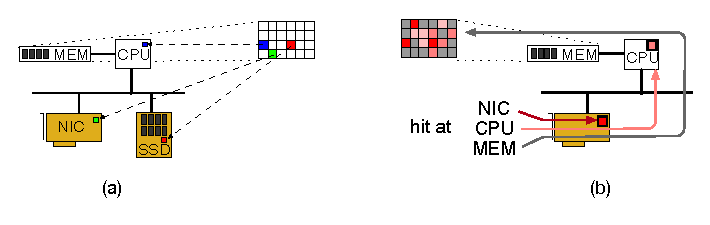
\includegraphics[bb=0 0 325 92]{fig_coherence.eps} %% 0.75
  \caption{Cache coherency scenarios: (a) a NIC and an SSD may be responsible
    for writing to specific addresses in memory that can be read by other
    elements, and (b) a NIC can be responsible for caching (and writing to) very
    hot pages while leaving the CPU responsible for less accessed pages.
  }
  \label{fig:coherence}
\end{figure}


At the time of writing, there are four upcoming interconnects offering both high speed and coherence:
CAPI~\cite{stuecheli15}, CCIX~\cite{ccix19}, CXL~\cite{cxl19} and
Gen-Z~\cite{knebel19}.
CCIX and Gen-Z support symmetric coherence, unlike CAPI or CXL, which support
asymmetric coherence.
CAPI is a competing standard to PCIe.
CCIX and CXL use only PCIe, while Gen-Z can use ethernet as well as PCIe.
The range of PCIe is short enough to work only within the confines of a chassis,
while ethernet allow to connect across chassis.
This opens up the possibility of CCIX or CXL being applied simultaneously with
Gen-Z to form coherence domains that cross server boundaries.


Cache coherency allows for new INC and NSP design use cases.
For instance, one may extend the caching hierarchy beyond the CPU.
Figure~\ref{fig:coherence}(b) illustrates this possibility.
Some distributed applications may cache hot data items in the
NIC~\cite{tokusashi18}.
With coherence, the NIC can also request write access to such an item and update
it.
Any other computing element that requests to cache that address would then see
the updates.


\section{Challenges and Opportunities}
\label{sec:challenges}

We mentioned above some immediate difficulties that arise when deploying current
generation INC and NSP platforms.
In this section, we elaborate on further challenges and opportunities that we
believe would unlock more of the potential of these platforms.


\softsubsec{In-Network Stateful Computations.}
%
Data management primarily involves stateful computations, i.e., algorithms that
access a result from a previous iteration and generate a new result at the
next one.
The aggregation operation discussed in Section~\ref{ssec:aggr} is one such
algorithm.
Maintaining state in-network, particularly in switches, is currently very
challenging.
Programmable switches rely on high-speed memories that, for cost reasons, are
present in limited amounts.
Moreover, switches have a very strict ``allowance'' of how many instructions
they can execute per packet and what those instructions can do.
These restrictions make maintaining data structures other than a hash
table on a switch possible but difficult.
Even some common operations on hash tables, such as collision management,
require some adapting, as we discussed above.


We miss a computing model that can relax those restrictions to a certain extent
while still keeping the ability to run logic at line-speed.
Supporting such a model would most likely require introducing new hardware onto
programmable switches.
We believe such a model is possible, but the field of in-network computing is
still new.
There is not yet a clear list of missing operations from applications beyond
networking protocols on which to base new switch hardware capabilities.


\softsubsec{SSD-Application Interface.}
%
A regular SSD makes several decisions such as IO scheduling and page mapping
based solely on observing the stream of IO commands it receives~\cite{nam11}.
When application logic executes inside the device, it becomes an additional
stream of IO commands.
The internal and external streams would likely compete with one another.
A straightforward way to manage the new internal streams is to pretend they came
from outside and to proceed as usual.


An alternative way would be to allow the application logic and the device to
interact.
Consider again the checkpoint derivation scenario we describe in
Section~\ref{ssec:cp_derivation}.
It generates new IO requests at a given pace.
Depending on the current load on the SSD, the checkpoint stream can be too fast or
too slow for the device to handle.
Ideally, we want a means for the device and the application logic to negotiate
that pace.
There is an opportunity here to establish a communication model that supports
this kind of interaction.


\softsubsec{SSD Channel Architecture.}
%
An SSD's bandwidth and capacity are a result of combining many relatively
limited NAND flash \emph{packages} (chips)~\cite{micheloni12}.
A typical arrangement is to group the packages in disjoint sets called
\emph{channels}.
There are anywhere between 8 to 32 channels in a typical SSD.
This arrangement has proved adequate when data pages are transferred in and out
of the device.


The introduction of application logic into an SSD, however, can cause data
pages to be moved \emph{across packages}---possibly between channels.
For instance, we describe in Section~\ref{ssec:cp_derivation} how an NSP process
can read pages from a transaction log and write them, after some manipulation,
as pages of a checkpoint.
In a traditional SSD architecture, this pattern would consume bandwidth from
both the origin and the destination channels.
We believe that there may be other package interconnect architectures
beyond channels that are more suited to the data movements above.
To the best of our knowledge, there has been no study about interconnects that
involve architectures other than fixed channels.


\softsubsec{Code-Variant Generation and Selection.}
%
INC and NSP platforms introduce additional hardware heterogeneity to computing
platforms.
An algorithm implementation that works well on a given switch may not work on a
different one, due to architectural differences.
The generation and selection of variant implementations is a known problem; it
appeared before in domains such as GPUs~\cite{rosenfeld15}.


To complicate matters, some algorithms are flexible enough to be deployed either
on a NIC or on the switch to which it connects.
The selection of the most appropriate platform constitutes an optimization step
that compounds to the variant selection problem above.
Currently, the programmer is responsible for making such choices.
There is an opportunity for creating higher-level tooling that would aid in
these decisions.


\softsubsec{Runtime Resource Management.}
%
In a regular setting, the operating system mediates every single network and
storage IO between applications and devices.
The OS does so by interposing itself between the two.
What, then, should be the role of the OS when a portion of the applications
reside \emph{inside} the device?


One potential solution is to accept that applications may want to access a device
directly, without mediation.
Such is the premise of Arrakis~\cite{peter15}, which tricks an application into
interacting with virtual versions of the devices, and redesigns the kernel to
provide the expected protections under such assumptions.


\section{Discussion}
\label{sec:discussion}

Notwithstanding the challenges and opportunities described in the previous
section, INC and NSP platforms are a reality.
The question arises as to whether they are ready for adoption.
In this section, we break this question into a list of sub-questions and answer
each one in turn.


\softsubsec{Are there diverse offerings of INC and NSP platforms?}
%
INC can be realized by many different hardware targets, both on switches and
NICs.
In terms of programmable switches, there are at least three silicon
manufacturers producing programmable ASICs: Barefoot (Intel)
Tofino~\cite{barefoot}, Broadcom Trident 4~\cite{broadcomT4}, and Cavium
(Marvel) Xpliant~\cite{cavium}.
Together, these chips appear in several commercial offerings from companies such as
Cisco and Arista.
SmartNICs are also widely available, ranging from FPGA-centric accelerators such as
Xilinx Alveo~\cite{xilinx} to more software-oriented platforms such as
Netronome~\cite{netronome}.
The offering for programming languages and abstractions is also diverse.
A prevalent language is \texttt{P4}~\cite{bosshart14}, but there are variations
such as \texttt{NPL}~\cite{broadcomnpl} and even \texttt{C} libraries in some
cases~\cite{netronome}.


NSP is also a rich environment with many prototyping and commercial platforms
available.
For instance, SSDs are starting to emerge that introduce application
specializations.
Samsung has recently announced the KV-SSD, which incorporates Key Value store
logic within its firmware~\cite{ki17}.
One issue with such offerings is that they add application functionality
but do not expose programmability.
The interested reader should look at~\cite{picoli20} for an extensive list of
specialized SSD and NSP-platforms available at the time of writing.


\softsubsec{What are the advantages of INC and NSP compared to ``CPU-centric''
alternatives?}
%
While there is no study yet of an exacale platform that resorts to both INC and
NSP, the expected benefits are a combination of increased performance, lower
energy expenditure, and lower CPU utilization.
There a numerous works that provide partial results.

For INC, data manipulations such as the one described in Section~\ref{ssec:aggr}
were studied before~\cite{lerner19}.
We can expect to see the performance of many typical queries improve by a factor of
2$\times$\ by using programmable switches at moderate network
speeds.
The power consumption in these switches is estimated to be only 12.4\% higher
than their fixed-function counterparts, and, anecdotally, the switches cost
about the same.
The operations-per-Watt ratio on some INC platforms such as smartNICs was
also studied before~\cite{tokusashi18}.
For instance, a variant of the caching scenario we discussed in
Section~\ref{sec:interconnects} reports a 17$\times$ better power utilization as
compared to a regular CPU.


NSP platforms deliver similar benefits.
According to~\cite{kim16}, the performance of scans and joins can see
performance improvements between 5$\times$ and 47$\times$, the cost of equipping
an SSD to support near-storage processing is less than 1\% of its total cost,
and the energy-efficiency compared to performing those operations on a CPU can be up
to 45$\times$ better.


\softsubsec{Are there standards in place to guarantee the portability and
longevity of the solutions?}
%
There is a big difference from a standardization point of view between INC and
NSP technologies.
As mentioned above, INC has broadly embraced \texttt{P4} as a programming language.
The latest edition of the language, \texttt{P4$_{16}$}, allows different target
platforms to express their capabilities.
A compiler can generate specific code from a unique source to different, maybe
even disparate, devices.
These feature makes the language flexible enough to work on future devices,
which can only help its adoption.


In contrast, there is not yet a consensus on how computational storage should be
programmed.
We even miss a standard around what an open-channel SSD should be, which would
arguably be a necessary step.


\section{Conclusion}
\label{sec:conclusion}

In this paper, we reviewed how the evolution of the network and storage stacks
have unlocked their computing power.
Applications can not only request services from these stacks, but also
embed logic into them.
We showed that with a careful redesign, algorithms running on INC or NSP
platforms could present a reduced amount of data movement, lower CPU
utilization, less energy consumption, or a combination of these.


We also discussed several challenges that INC and NSP still face.
Despite these limitations, we commented on a current generation of INC- and
NSP-enabled devices that are available off-the-shelf.
We believe that the emergence of the network and storage stacks as computing
elements creates promising ways to scale typical data management computations.


\softsec{Acknowledgments.}
%
This project has received funding from the European Research Council (ERC) under
the European Unions Horizon 2020 research and innovation programme (grant
agreement 683253/GraphInt).


\begin{thebibliography}{10}
\itemsep=1pt
\begin{small}

\bibitem{barefoot}
  \newblock Barefoot Tofino and Tofino 2 Switches.
  \newblock https://www.barefootnetworks.com/products/brief-tofino-2/.

\bibitem{bifulco18} R.~Bifulco, and G.~R\'etv\'ari.
  \newblock A Survey on the Programmable Data Plane: Abstractions, Architectures, and Open Problems.
  \newblock {\em HPSR}, June, 2018.

\bibitem{bjorling17} M.~Bj{\o}ling, J.~Gonz\'alez, and P.~Bonnet.
  \newblock Lightnvm: The Linux Open-Channel SSD Subsystem
  \newblock {\em FAST}, February, 2017.

\bibitem{broadcomnpl} Broadcom NPL.
  \newblock Network Programming Language.
  \newblock {\em https://nplang.org/}.

\bibitem{broadcomT4} Broadcom.
  \newblock Broadcom Trident 4.
  \newblock {\em https://www.broadcom.com/products/ethernet-connectivity/switching/strataxgs/bcm56880-series}.

\bibitem{bosshart13} P.~Bosshart, G.~Gibb, H.-S.~Kim, G.~Varghese, N.~McKeown, M.~Izzard, F.~Mujica, and M.~Horowitz.
  \newblock Forwarding Metamorphosis: Fast Programmable Match-Action Processing in Hardware for SDN.
  \newblock {\em SIGCOMM CCR}, 43(4):99--110, 2013.

\bibitem{bosshart14} P.~Bosshart., D.~Daly, G.~Gibb, M.~Izzard, N.~McKeown, J.~Rexford, C.~Schlesinger, D.~Talayco, A.~Vahdat, G.~Varghese, and D.~Walker.
  \newblock P4: Programming protocol-independent packet processors.
  \newblock {\em ACM SIGCOMM CCR}, 44(3):87--95, 2014.

\bibitem{budruk03} R.~Budruk, D.~Anderson, and E.~Solari.
  \newblock PCI Express System Architecture.
  \newblock {\em Pearson Education}, 2003.

\bibitem{cai17} Y.~Cai, S.~Ghhose, E.F.~Haratsch, Y.~Luo, and O.~Mutlu.
  \newblock Error Characterization, Mitigation, and Recovery in Flash-Memory-Based Solid-State Drives.
  \newblock {\em Proc. of the IEEE}, 105(9), 1666--1704, 2017.

\bibitem{calvert98} K.L.~Calvert, S.~Bhattacharjee, E.~Zegura, and J.~Sterbenz.
  \newblock Directions in Active Networks.
  \newblock {\em IEEE Comm. Magazine}, 36(10):72--78, 1998.

\bibitem{cavium} Cavium.
  \newblock XPliant Ethernet Switch Product Family.
  \newblock {\em www.cavium.com/XPliant-Ethernet-Switch-Product-Family.html}

\bibitem{ccix19} CCIX Consortium.
  \newblock An Introduction to CCIX.
  \newblock {\em White Paper}, https://www.ccixconsortium.com/wp-content/uploads/2019/11/CCIX-White-Paper-Rev111219.pdf

\bibitem{chung09} T.-S.~Chung, D.-J.~Park, S.~Park, D.-H.~Lee, S.-W.~Lee, and H.-J.~Song.
  \newblock A Survey of Flash Translation Layer.
  \newblock {\em J. of Syst. Archit.}, 55(5--6):332--343, 2009.

\bibitem{cxl19} D.D.~Sharma.
  \newblock An Introduction to Compute Express Link.
  \newblock {\em White Paper}, https://docs.wixstatic.com/ugd/0c1418\_d9878707bbb7427786b70c3c91d5fbd1.pdf.

\bibitem{do13} J.~Do, Y.S.~Kee, J.M.~Pzatel, C.~Park, K.~Park, and D.J.~DeWitt.
  \newblock Query Processing on Smart SSDs: Opportunities and Challenges.
  \newblock {\em SIGMOD}, June, 2013.

\bibitem{do19} J.~Do, S.~Sengupta, and S.~Swanson.
  \newblock Programmable Solid-State Storage in Future Could Datacenters.
  \newblock {\em CACM}, 62(6):54--62, 2019.

\bibitem{fang19} J.~Fang, Y.T.B.~Mulder, J.~Hidders, J.~Lee, and H.P.~Hofstee.
  \newblock In-Memory Database Acceleration on FPGAs: A Survey.
  \newblock {\em VLDB Journal}, October, 2019.

\bibitem{gu16} B.~Gu, A.S.~Yoon, D.H.~Bae, I.~Jo, J.~Lee, and J.~Yoon.
  \newblock Biscuit: A Framework for Near-Data Processing of Big Data Workloads.
  \newblock {\em SIGARCH Comp. Arch. News}, 44(3):153--165.

\bibitem{guz18} Z.~Guz, H.~Li, A.~Shayesteh, and V.~Balakrishnan.
  \newblock Performance Characterization of NVMe-over-Fabrics Storage Disaggregation.
  \newblock {\em ACM Trans. on Storage}, 14(4):1553--3077, 2018.

\bibitem{ki17} Y.-S.~Ki.
  \newblock Key Value SSD Explained – Concept, Device, System, and Standard.
  \newblock {\em SNIA SDC}, September, 2017.

\bibitem{kim16} S.~Kim, H.~Oh, C.~Park, S.~Cho, S.-W.~Lee, and B.~Moon.
  \newblock In-Storage Processing of Database Scans and Joins.
  \newblock {\em Inf. Sci.}, 327(C):183--200, 2016.

\bibitem{knebel19} P.~Knebel, D.~Berkram, A.~Davis, D.~Emmot, P.~Faraboschi, and G.~Gostin.
  \newblock Gen-Z Chipset for Exascale Fabrics.
  \newblock {\em HotChips}, August, 2019.

\bibitem{kreutz15} D.~Kreutz, F.M.V.~Ramos, P.E.~Ver\'issimo, C.E.~Rothenberg, S.~Azodolmolky, and S.~Uhlig.
  \newblock Software-Defined Networking: A Comprehensive Survey.
  \newblock {\em Proc. of the IEEE}, 103(1):14--76, 2015.

\bibitem{kwak20} J.~Kwak, S.~Lee, K.~Park, J.~Jeong, and Y.H.~Song.
  \newblock Cosmos+ OpenSSD: Rapid Prototype for Flash Storage Systems.
  \newblock {\em ACM Trans. on Storage}, to appear.

\bibitem{lerner19} A.~Lerner, R.~Russein, and P.~Cudr\'e-Mauroux.
  \newblock The Case for Network Accelerated Query Processing.
  \newblock {\em CIDR}, January, 2019.

\bibitem{lerner20} A.~Lerner, J.~Kwak, S.~Lee, K.~Park, Y.H.~Song, and P.~Cudr\'e-Mauroux.
  \newblock It Takes Two: Instrumenting the Interaction between In-Memory Databases and Solid-State Drives.
  \newblock {\em CIDR}, January, 2020.

\bibitem{micheloni12} R.~Micheloni, A.~Marelli, and S.~Eshghi.
  \newblock Inside Solid State Drives (SSDs).
  \newblock {\em Springer}, 2012.

\bibitem{nam11} E.H.~Nam, B. S. J.~Kim, H.~Eom, and S. L.~Min.
  \newblock Ozone (O3): An Out-of-Order Flash Memory Controller Architecture.
  \newblock {\em IEEE Transactions on Computers}, 60(5):653--666, 2011.

\bibitem{netronome} Netronome.
  \newblock Agilio CX SmartNICs.
  \newblock {\em https://www.netronome.com/products/agilio-cx/}

\bibitem{ouyang14} J.~Ouyang, S.~Lin, S.~Jiang, Z.~Hou, Y.~Wang, and Y.~Wang.
  \newblock SDF: Software-Defined Flash for Web-Scale Internet Storage Systems.
  \newblock {\em ASPLOS}, 2014.

\bibitem{peter15} S.~Peter, J.~Li, I.~Zhang, D.R.K.~Ports, D.~Woos, A.~Krishnamurthy, T.~Anderson, and T.~Roscoe.
  \newblock Arrakis: The Operating System Is the Control Plane.
  \newblock {\em ACM TOCS}, 33(4), 2015.

\bibitem{picoli19} I.L.~Picoli, P.~Bonnet, and P.~T\"oz\"un.
  \newblock LSM Management on Computational Storage.
  \newblock {\em DaMoN}, July, 2019.

\bibitem{picoli20} I.L.~Picoli, N.~Hedam, P.~Bonnet, and P.~T\"oz\"un.
  \newblock Open-Channel SSD (What Is It Good For).
  \newblock {\em CIDR}, January, 2020

\bibitem{ports19} D.R.K.~Ports, and J.~Nelson.
  \newblock When Should The Network Be The Computer.
  \newblock {\em HotOS}, May, 2019.

\bibitem{riedel01} E.~Riedel, C.~Faloutsos, G.A.~Gibson, and D.~Nagle.
  \newblock Active Disks for Large-Scale Data Processing.
  \newblock {\em IEEE Computer}, 34(6):68--74, 2001.

\bibitem{rosenfeld15} V.~Rosenfeld, M.~Heimel, C.~Viebig, and V.~Markl.
  \newblock The Operator Variant Selection Problem on Hetergoneous Hardware.
  \newblock {\em ADMS}, August, 2015.

\bibitem{ruan19} Z.~Ruan, T.~He, and J.~Cong.
  \newblock INSIDER: Designing In-Storage Computing System for Emerging High-Performance Drive.
  \newblock {\em Usenix ATC}, July, 2019.

\bibitem{sivaraman16} A.~Sivaraman, A.~Cheung, M.~Budiu, C.~Kim, M.~Alizadeh, H.~Balakrishnan, G.~Varghese, N.~McKeown, and S.~Licking.
  \newblock Packet transactions: High-level programming for line-rate switches.
  \newblock {\em SIGCOMM}, August, 2016.

\bibitem{stuecheli15} J.~Stuecheli, B.~Blaner, C.R.~Johns, and M.S.~Siegel.
  \newblock CAPI: A Coherent Accelerator Processor Interface.
  \newblock {\em IBM Journal of Research and Development}, 59(1):1--7, 2015.

\bibitem{teubner13} J.~Teubner, and L.~Woods.
  \newblock Data Processing on FPGAs.
  \newblock {\em Morgan \& Claypool Publishers}, 2013.

\bibitem{tokusashi18} Y.~Tokusashi, H.~Matsutani, and N.~Zilberman.
  \newblock LaKe: The Power of In-Network Computing.
  \newblock {\em ReConFig}, December, 2018.

\bibitem{xilinx} Xilinx.
  \newblock ALVEO Adaptable Accelerator Cards for Data Center Workloads.
  \newblock {\em https://www.xilinx.com/content/xilinx/en/products/boards-and-kits/alveo.html}

\bibitem{woods14} L.~Woods, Z.~Istv\'an, and G.~Alonso.
  \newblock Ibex: An Inteligent Storage Engine with Support for Advanced SQL Offloading.
  \newblock {\em Proc. of the VLDB}, 7(11):963--974.

\bibitem{zilberman14} N.~Zilberman, Y.~Audzevich, G.A.~Covington, and A.W.~Moore.
  \newblock NetFPGA SUME: Towards 100 Gbps as Research Commodity.
  \newblock {\em IEEE Micro}, 34(5):32--41, 2014.

\end{small}
\end{thebibliography}

\end{document}

\end{article}

\end{articlesection}

% put the news items below- there can be multiple news sections
% each with its own title
% news will usually have an author as well as a title, 
% e.g. TCDE elections
% news articles are in the same format as letters
% typically, news articles will be stored in a directory called "news"

%\begin{newssection}{News headline}

% insert news items here; news will typically have authors
% see the Sept. 2018 issue for an example

%\begin{news}{news item title}
%{author name}{author affiliation}
%\input{news/news-article.tex}
%\end{news}
%
%\newpage


%\end{newssection}



\begin{callsection}

%  This section will be empty for your version
%
%  Calls for papers section.  Use the callsection environment.
%  Each call for papers is contained in an call environment, where the single 
%  required options to \begin{call} is the name of the conference.
% typically calls are stored in a "calls" directory
%
%\begin{call}{name of conference}
%\centerline{\includegraphics[width=\textwidth, bb= 0 0 590 760]{calls/conference-name.pdf}}
%\end{call}
%\begin{call}{ICDE 2019 Conference}
%\centerline{\includegraphics[width=\textwidth, bb= 0 0 610 790] {../Dec-2018/calls/icde19.pdf}} 
%\centerline{\includegraphics[width=\textwidth, bb= 0 0 590 760] {calls/icde19.pdf}}
%\end{call}
\begin{call}{TCDE Membership Form}
%\centerline{\includegraphics[width=\textwidth, bb= 0 0 610 790]
\centerline{
\includegraphics[width=\textwidth, bb= 0 0 590 760] {../Dec-2018/calls/tcde.pdf}}
\end{call}

\end{callsection}

\end{bulletin}
\end{document}
